
\documentclass[oneside,english]{book}
\usepackage[T1]{fontenc}
%% DK DK we do not accept accented letters, use the old LaTeX syntax
%% DK DK for them instead: \'e \`e  \"e \^e and so on.
%% DK DK \usepackage[latin1]{inputenc}
\usepackage[letterpaper]{geometry}
\geometry{verbose,tmargin=1in,bmargin=1in,lmargin=1in,rmargin=1in}

% table of contents and numbering
\usepackage{tocbibind}
\setcounter{secnumdepth}{3}
\setcounter{tocdepth}{3}

\usepackage{babel}
\usepackage{float}
\usepackage{textcomp}
\usepackage{amsmath}
\usepackage{amssymb}

\IfFileExists{url.sty}{\usepackage{url}}
                      {\newcommand{\url}{\texttt}}

% biblio
\usepackage[authoryear]{natbib}
% biblio GJI
\bibliographystyle{abbrvnat}

% fonts
\usepackage{times}

% figures
\usepackage[pdftex]{graphicx}

% we are running pdflatex, so convert .eps files to .pdf
%\usepackage{epstopdf}

% colors to show the corrections
\usepackage[dvipsnames,usenames]{xcolor}
\definecolor{light-gray}{rgb}{0.7,0.7,0.7}
\definecolor{dark-gray}{rgb}{0.1,0.1,0.3}
\definecolor{light-blue}{rgb}{0.7,0.7,0.9}
\definecolor{dark-blue}{rgb}{0.2,0.2,0.5}

% hyperlinks to sections and references
\usepackage[pdftex]{hyperref}
% more options
\hypersetup{
  bookmarks=true,
  bookmarksnumbered=true,
  pdfpagemode=UseNone,
  pdfstartview=FitH,
  pdfpagelayout=SinglePage,
  pdfborder={0 0 0},
  colorlinks=true,      % color links
  citecolor=dark-gray,  % citation links
  filecolor=dark-gray,  % file links
  linkcolor=dark-gray,  % internal link (rgb values)
  urlcolor=dark-blue    % external weblinks
}

% tables
\usepackage{longtable}

\usepackage{varioref}
\usepackage{booktabs}

% Latex generated graphics
\usepackage{tikz}
\usetikzlibrary{trees}

% create thumbnails
%\usepackage[pdftex]{thumbpdf}

\makeatletter

%%%%%%%%%%%%%%%%%%%%%%%%%%%%%% LyX specific LaTeX commands.
%% Because html converters don't know tabularnewline
\providecommand{\tabularnewline}{\\}

%%%%%%%%%%%%%%%%%%%%%%%%%%%%%% Textclass specific LaTeX commands.
\newenvironment{lyxcode}
{\begin{list}{}{
\setlength{\rightmargin}{\leftmargin}
\setlength{\listparindent}{0pt}% needed for AMS classes
\raggedright
\setlength{\itemsep}{0pt}
\setlength{\parsep}{0pt}
\normalfont\ttfamily}%
 \item[]}
{\end{list}}

%%%%%%%%%%%%%%%%%%%%%%%%%%%%%% User specified LaTeX commands.

% colors for the text
\newcommand{\red}[1]{\textcolor{Red}{#1}}

% hyperlinks to sections and references
%\newcommand{\urlwithparentheses}[1]{(\url{#1})}

\newcommand{\toall}[1]{\textbf{*** All: #1 ***}}
\newcommand{\tojeroen}[1]{\textbf{*** Jeroen: #1 ***}}
\newcommand{\tobrian}[1]{\textbf{*** Brian: #1 ***}}
\newcommand{\tovala}[1]{\textbf{*** Vala: #1 ***}}
\newcommand{\tovalabrian}[1]{\textbf{*** Vala \& Brian: #1 ***}}
\newcommand{\tovalaqinya}[1]{\textbf{*** Vala \& Qinya: #1 ***}}
\newcommand{\toqinya}[1]{\textbf{*** Qinya: #1 ***}}
\newcommand{\tomin}[1]{\textbf{*** Min: #1 ***}}
\newcommand{\toalessia}[1]{\textbf{*** Alessia: #1 ***}}
\newcommand{\todimitri}[1]{\textbf{*** Dimitri: #1 ***}}

\newcommand{\nexxi}{\mbox{\texttt{NEX\_XI}}}
\newcommand{\nexeta}{\mbox{\texttt{NEX\_ETA}}}
\newcommand{\nprocxi}{\mbox{\texttt{NPROC\_XI}}}
\newcommand{\nproceta}{\mbox{\texttt{NPROC\_ETA}}}
\newcommand{\nchunks}{\mbox{\texttt{NCHUNKS}}}

% BibTeX logo
\newcommand{\BibTeX}{{\rm B\kern-.05em{\sc i\kern-.025em b}\kern-.08em{T}\kern-.1667em\lower.7ex\hbox{E}\kern-.125emX}}

\makeatother

%%%%%%%%%%%%%%%%%%%%%%%%%%%%%% Start of document.

\begin{document}

%%%%%%%%%%%%%%%%%%%%%%%%%%%%%%%%%%%%%%%%%%%
%% Title
%%%%%%%%%%%%%%%%%%%%%%%%%%%%%%%%%%%%%%%%%%%

\thispagestyle{empty}
\begin{center}
\vspace*{-1.8truecm}
\noindent\makebox[\textwidth]{\noindent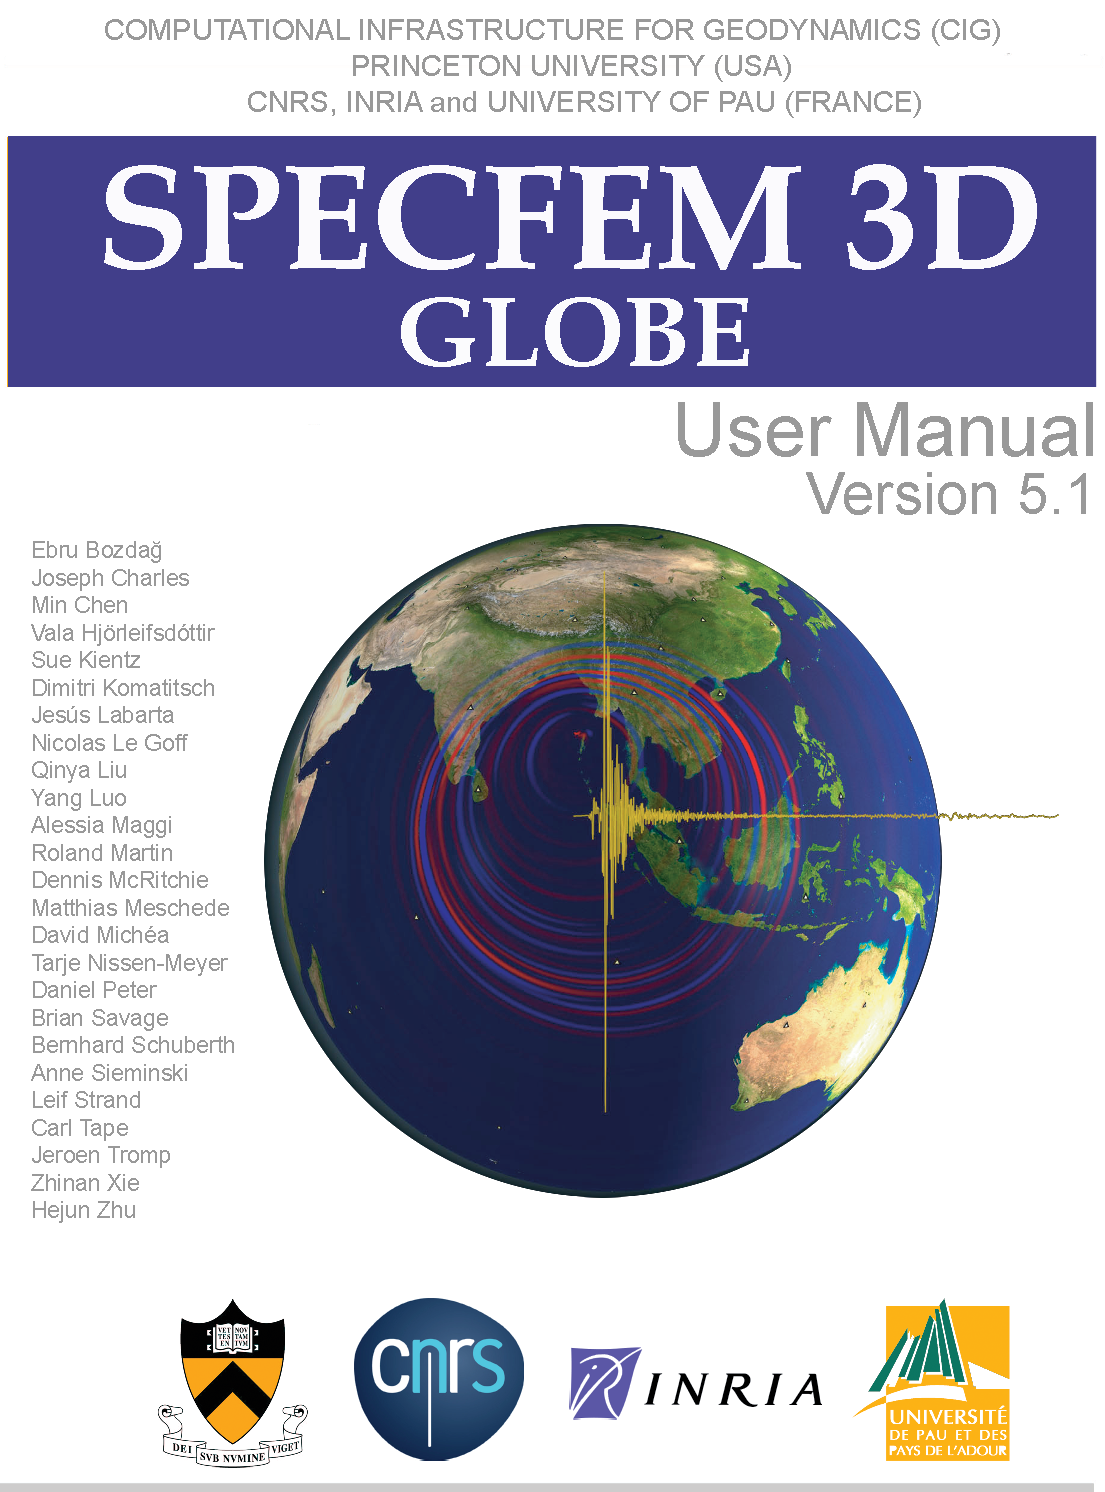
\includegraphics[width=0.83\paperwidth]{figures/specfem_3d_globe-cover.pdf}}
\end{center}
%
\title{\thispagestyle{empty}\textbf{SPECFEM3D\_GLOBE}\\
\textbf{User Manual}}
%
\author{$\copyright$ Princeton University (USA) and CNRS / University of Marseille (France),\\
ETH Z\"urich (Switzerland),\\
Version 8 . 0
}

% date of last edit
\date{\today}

\maketitle

%%%%%%%%%%%%%%%%%%%%%%%%%%%%%%%%%%%%%%%%%%

\section*{Authors}

\noindent The SPECFEM3D package was first developed by Dimitri
Komatitsch and Jean-Pierre Vilotte at Institut de Physique du Globe
(IPGP) in Paris, France from 1995 to 1997 and then by Dimitri Komatitsch
and Jeroen Tromp at Harvard University and Caltech, USA, starting in 1998.
The story started on April 4, 1995, when Prof. Yvon Maday from CNRS and University of Paris, France, gave a lecture to
Dimitri Komatitsch and Jean-Pierre Vilotte at IPG about the nice properties of the Legendre spectral-element method with diagonal mass matrix that he had used for
other equations. We are deeply indebted and thankful to him for that.
That followed a visit by Dimitri Komatitsch to OGS (Istituto Nazionale di Oceanografia e di Geofisica Sperimentale) in Trieste, Italy, in February 1995
to meet with G\'eza Seriani and Enrico Priolo, who introduced him to their 2D Chebyshev version of the spectral-element method with a non-diagonal mass matrix.
We are deeply indebted and thankful to them for that.\newline

%%%%%%%% please do NOT merge the lines of the paragraph below, it makes it difficult to insert new names in alphabetical order; leave a single name per line
%%%%%%%% please do NOT merge the lines of the paragraph below, it makes it difficult to insert new names in alphabetical order; leave a single name per line
%%%%%%%% please do NOT merge the lines of the paragraph below, it makes it difficult to insert new names in alphabetical order; leave a single name per line
Since then it has been developed and maintained by a development team: in alphabetical order,
Michael Afanasiev,
Dmitry Alexeev,
Jean-Paul (Pablo) Ampuero,
Kazuto Ando,
Kangchen Bai,
Piero Basini,
Stephen Beller,
C\'eline Blitz,
Alexis Bottero,
Ebru Bozda\u{g},
Emanuele Casarotti,
Joseph Charles,
Min Chen,
Paul Cristini,
Congyue Cui,
Cl\'ement Durochat,
Percy Galvez,
Hom Nath Gharti,
Dominik G\"oddeke,
Leopold Grinberg,
Vala Hj\"orleifsd\'ottir,
Elodie Kendall,
Sue Kientz,
Dimitri Komatitsch,
Jes\'us Labarta,
Piero Lanucara,
Nicolas Le Goff,
Pieyre Le Loher,
Matthieu Lefebvre,
Qinya Liu,
Youshan Liu,
David Luet,
Yang Luo,
Alessia Maggi,
Federica Magnoni,
Roland Martin,
Ren\'e Matzen,
Dennis McRitchie,
Jean-Fran\c{c}ois M\'ehaut,
Matthias Meschede,
Peter Messmer,
David Mich\'ea,
Takayuki Miyoshi,
Vadim Monteiller,
Surendra Nadh Somala,
Tarje Nissen-Meyer,
Ridvan Orsvuran,
Laura Parisi,
Daniel Peter,
Kevin Pouget,
Max Rietmann,
Vittorio Ruggiero,
Elliott Sales de Andrade,
Brian Savage,
Bernhard Schuberth,
Anne Sieminski,
James Smith,
Leif Strand,
Carl Tape,
Jeroen Tromp,
Seiji Tsuboi,
Brice Videau,
Jean-Pierre Vilotte,
Zhinan Xie,
Chang-Hua Zhang,
Hejun Zhu.\newline


The cover graphic of the manual was created by Santiago Lombeyda from
Caltech's Center for Advanced Computing Research (CACR), USA, with free satellite clipart pictures
from \url{http://www.4vector.com} and \url{http://www.clker.com} added to it.\newline

The code is released open-source under the GNU version 3 license, see the license at the end of this manual.\newline



\newpage{}

\section*{Current and past main participants or main sponsors of the SPECFEM project (in no particular order)}
%
\begin{figure}[htbp]
\noindent \begin{centering}

\includegraphics[width=0.125\textwidth]{figures/logo_cnrs.png}\vspace*{2truemm}

\includegraphics[width=0.125\textwidth]{figures/logo_princeton.jpg}\vspace*{2truemm}

\includegraphics[width=0.15\textwidth]{figures/logo_aix_marseille_universite.png}\vspace*{0.02truemm}

\includegraphics[width=0.15\textwidth]{figures/logo_ETH.jpg}\vspace*{2truemm}

\includegraphics[width=0.12\textwidth]{figures/logo_CSC_China.jpg}\vspace*{0.02truemm}

\includegraphics[width=0.15\textwidth]{figures/logo_inria.jpg}\vspace*{2truemm}

\includegraphics[width=0.14\textwidth]{figures/logo_UPPA.png}
\par\end{centering}
%
\vspace*{-2truemm}
%
\noindent \begin{centering}

\includegraphics[width=0.15\textwidth]{figures/logo_NVIDIA.jpg}\vspace*{2truemm}

\includegraphics[width=0.125\textwidth]{figures/logo_IUF.jpg}\vspace*{2truemm}

\includegraphics[width=0.135\textwidth]{figures/logo_Caltech.png}\vspace*{2truemm}

\includegraphics[width=0.135\textwidth]{figures/logo_Harvard.jpg}\vspace*{2truemm}

\includegraphics[width=0.135\textwidth]{figures/logo_IPGP.jpg}\vspace*{2truemm}

\includegraphics[width=0.112\textwidth]{figures/logo_ANR.png}\vspace*{2truemm}

\includegraphics[width=0.112\textwidth]{figures/logo_NSF.png}\vspace*{2truemm}
\par\end{centering}
%
\vspace*{-2truemm}
%
\noindent \begin{centering}

\includegraphics[width=0.190\textwidth]{figures/logo_European_Union.png}\vspace*{2truemm}

\includegraphics[width=0.112\textwidth]{figures/logo_GENCI.jpg}\vspace*{2truemm}

\includegraphics[width=0.112\textwidth]{figures/logo_PRACE.jpg}\vspace*{2truemm}

\includegraphics[width=0.112\textwidth]{figures/logo_CINES.png}\vspace*{2truemm}

\includegraphics[width=0.130\textwidth]{figures/logo_Oak_Ridge.png}\vspace*{2truemm}
\hspace*{3mm}
\includegraphics[width=0.130\textwidth]{figures/logo_fondation_Del_Duca.png}\vspace*{2truemm}

\includegraphics[width=0.130\textwidth]{figures/logo_CIG.png}\vspace*{2truemm}
\par\end{centering}
%
\vspace*{-2truemm}
%
\noindent \begin{centering}

\includegraphics[width=0.112\textwidth]{figures/logo_University_of_Toronto.jpg}\vspace*{2truemm}

\includegraphics[width=0.109\textwidth]{figures/logo_INGV.jpg}\vspace*{2truemm}

\includegraphics[width=0.102\textwidth]{figures/logo_Univ_Toulouse.jpg}\vspace*{2truemm}

\includegraphics[width=0.112\textwidth]{figures/logo_TOTAL.jpg}\vspace*{2truemm}

\includegraphics[width=0.130\textwidth]{figures/logo_Fairbanks.jpg}\vspace*{2truemm}

\includegraphics[width=0.120\textwidth]{figures/logo_CINECA.jpg}\vspace*{2truemm}

\includegraphics[width=0.140\textwidth]{figures/logo_Intel_Exascale_Labs.png}\vspace*{2truemm}

\includegraphics[width=0.130\textwidth]{figures/logo_Maison_Simulation.jpg}
\par\end{centering}
\end{figure}



%%%%%%%%%%%%%%%%%%%%%%%%%%%%%%%%%%%%%%%%%%%
%% Table of contents
%%%%%%%%%%%%%%%%%%%%%%%%%%%%%%%%%%%%%%%%%%%

\newpage{}

\tableofcontents{}

%%%%%%%%%%%%%%%%%%%%%%%%%%%%%%%%%%%%%%%%%%%

\chapter{Introduction}

The software package SPECFEM3D\_GLOBE simulates three-dimensional global and regional seismic wave propagation
and performs full waveform imaging (FWI) or adjoint tomography based upon the spectral-element method (SEM).
The SEM is a continuous Galerkin technique \citep{TrKoLi08,PeKoLuMaLeCaLeMaLiBlNiBaTr11},
which can easily be made discontinuous \citep{BeMaPa94,Ch00,KoWoHu02,ChCaVi03,LaWaBe05,Kop06,WiStBuGh10,AcKo11};
it is then close to a particular case of the discontinuous Galerkin technique \citep{ReHi73,LeRa74,Arn82,JoPi86,BoMaHe91,FaRi99,HuHuRa99,CoKaSh00,GiHeWa02,RiWh03,MoRi05,GrScSc06,AiMoMu06,BeLaPi06,DuKa06,DeSeWh08,PuAmKa09,WiStBuGh10,DeSe10,EtChViGl10}, with optimized efficiency because of its tensorized basis functions \citep{WiStBuGh10,AcKo11}.
In particular, it can accurately handle very distorted mesh elements \citep{OlSe11}.\newline


It has very good accuracy and convergence properties \citep{MaPa89,SePr94,DeFiMu02,Coh02,DeSe07,SeOl08,AiWa09,AiWa10,MeStTh12}.
The spectral element approach admits spectral rates of convergence and allows exploiting $hp$-convergence schemes.
It is also very well suited to parallel implementation on very large supercomputers \citep{KoTsChTr03,TsKoChTr03,KoLaMi08a,CaKoLaTiMiLeSnTr08,KoViCh10} as well as on clusters of GPU accelerating graphics cards \citep{Kom11,MiKo10,KoMiEr09,KoErGoMi10}. Tensor products inside each element can be optimized to reach very high efficiency \citep{DeFiMu02}, and mesh point and element numbering can be optimized to reduce processor cache misses and improve cache reuse \citep{KoLaMi08a}. The SEM can also handle triangular (in 2D) or tetrahedral (in 3D) elements \citep{WinBoyd96,TaWi00,KoMaTrTaWi01,Coh02,MeViSa06} as well as mixed meshes, although with increased cost and reduced accuracy in these elements, as in the discontinuous Galerkin method.\newline


Note that in many geological models in the context of seismic wave propagation studies
(except for instance for fault dynamic rupture studies, in which very high frequencies or supershear rupture need to be modeled near the fault, see e.g. \cite{BeGlCrViPi07,BeGlCrVi09,PuAmKa09,TaCrEtViBeSa10})
a continuous formulation is sufficient because material property contrasts are not drastic and thus
conforming mesh doubling bricks can efficiently handle mesh size variations \citep{KoTr02a,KoLiTrSuStSh04,LeChLiKoHuTr08,LeChKoHuTr09,LeKoHuTr09}.
This is particularly true at the scale of the full Earth.\newline


For a detailed introduction to the SEM as applied to
global and regional seismic wave propagation, please consult \citet{TrKoLi08,PeKoLuMaLeCaLeMaLiBlNiBaTr11,KoVi98,KoTr99,Ch00,KoTr02a,KoTr02b,KoRiTr02,ChCaVi03,CaChViMo03,ChVa04,ChKoViCaVaFe07}.
A detailed theoretical analysis of the dispersion
and stability properties of the SEM is available in \citet{Coh02}, \citet{DeSe07}, \citet{SeOl07}, \citet{SeOl08} and \citet{MeStTh12}.\newline


Effects due to lateral variations in compressional-wave
speed, shear-wave speed, density, a 3D crustal model, ellipticity,
topography and bathymetry, the oceans, rotation, and self-gravitation are included.
The package can accommodate full 21-parameter anisotropy \citep{ChTr07}
as well as lateral variations in attenuation \citep{SaKoTr10}. Adjoint
capabilities and finite-frequency kernel simulations are also included
\citep{TrKoLi08,PeKoLuMaLeCaLeMaLiBlNiBaTr11,LiTr06,LiTr08,FiIgBuKe09,ViOp09}.\newline


The SEM was originally developed in computational fluid dynamics \citep{Pat84,MaPa89}
and has been successfully adapted to address problems in seismic wave propagation.
Early seismic wave propagation applications of the SEM, utilizing Legendre basis functions and a
perfectly diagonal mass matrix, include \cite{CoJoTo93}, \cite{Kom97},
\cite{FaMaPaQu97}, \cite{CaGa97}, \cite{KoVi98} and \cite{KoTr99},
whereas applications involving Chebyshev basis functions and a nondiagonal mass matrix
include \cite{SePr94}, \cite{PrCaSe94} and \cite{SePrPr95}.
In the Legendre version that we use in SPECFEM the mass matrix is purposely slightly inexact but diagonal (but can be made exact if needed, see \cite{Teu15}),
while in the Chebyshev version it is exact but non diagonal.\newline


Beware that, in a spectral-element method, some spurious modes (that have some similarities with classical so-called "Hourglass modes" in finite-element techniques,
although in the SEM they are not zero-energy modes) can appear in some (but not all) cases in the spectral element in which the source is located.
Fortunately, they do not propagate away from the source element.
However, this means that if you put a receiver in the same spectral element as a source, the recorded signals may in some cases be wrong, typically exhibiting some spurious
oscillations, which are often even non causal.
If that is the case, an easy option is to slightly change the mesh in the source region in order to get rid of these Hourglass-like spurious modes,
as explained in \cite{DuLiScGa14}, in which this phenomenon is described in details, and in which practical solutions to avoid it are suggested.\newline


SPECFEM3D\_GLOBE can now perform gravity field calculations in addition (or instead of) seismic wave propagation only.
See flag \texttt{GRAVITY\_INTEGRALS} in file \texttt{setup/constants.h.in}. Please also refer to \citet{Martin2017}.
And yes, that is the reason why there is a gravity observation satellite on the cover of the manual :-)\newline


All SPECFEM3D\_GLOBE software is written in Fortran2003 with full portability
in mind, and conforms strictly to the Fortran2003 standard. It uses
no obsolete or obsolescent features of Fortran. The package uses
parallel programming based upon the Message Passing Interface (MPI)
\citep{GrLuSk94,Pac97}.\newline


SPECFEM3D\_GLOBE won the Gordon Bell award for best performance at the SuperComputing~2003
conference in Phoenix, Arizona (USA) (see \cite{KoTsChTr03}).
It was a finalist again in 2008 for a run at 0.16 petaflops (sustained) on 149,784 processors of the `Jaguar' Cray XT5 system at Oak Ridge National Laboratories (USA) \citep{CaKoLaTiMiLeSnTr08}.
It also won the BULL Joseph Fourier supercomputing award in 2010.\newline


It reached the sustained one petaflop performance level for the first time in February 2013
on the Blue Waters Cray supercomputer at the National Center for Supercomputing Applications (NCSA), located at the University of Illinois at Urbana-Champaign (USA).\newline


The package includes support for GPU graphics card acceleration \citep{Kom11,MiKo10,KoMiEr09,KoErGoMi10} and also supports OpenCL.\newline

%% future plans:
%% better see https://github.com/SPECFEM/specfem3d_globe/wiki/Development-plan

%The next release of the code will include support for
%Convolutional or Auxiliary Differential Equation Perfectly Matched absorbing Layers (C-PML or ADE-PML)
%\citep{MaKoEz08,MaKoGe08,MaKo09,MaKoGeBr10,KoMa07} for the case of single-chunk simulations in regional models.

\section{Citation}

You can find all the references below in \BibTeX format in file \texttt{doc/USER\_MANUAL/bibliography.bib}.\newline


If you use SPECFEM3D\_GLOBE for your own research, please cite at least one
of the following articles: \cite{KoXiBoPeSaLiTr16,TrKoLi08,PeKoLuMaLeCaLeMaLiBlNiBaTr11,VaCaSaKoVi99,LeChLiKoHuTr08,LeChKoHuTr09,LeKoHuTr09,KoMiEr09,KoErGoMi10,WiKoScTr04,KoLiTrSuStSh04,ChKoViCaVaFe07,MaKoDi09,KoViCh10,CaKoLaTiMiLeSnTr08,TrKoHjLiZhPeBoMcFrTrHu10,KoRiTr02,KoTr02a,KoTr02b,KoTr99} or \cite{KoVi98}.\newline


If you use the C-PML absorbing layer capabilities of the code, please cite at least one article
written by the developers of the package, for instance:
%
\begin{itemize}
\item \cite{XiKoMaMa14},
\item \cite{XiMaCrKoMa16}.
\end{itemize}
%
If you use the UNDO\_ATTENUATION option of the code in order to produce full anelastic/viscoelastic sensitivity kernels, please cite at least one article
written by the developers of the package, for instance (and in particular):
%
\begin{itemize}
\item \cite{KoXiBoPeSaLiTr16}.
\end{itemize}
%
More generally, if you use the attenuation (anelastic/viscoelastic) capabilities of the code, please cite at least one article
written by the developers of the package, for instance:
%
\begin{itemize}
\item \cite{KoXiBoPeSaLiTr16},
\item \cite{BlKoChLoXi16}.
\end{itemize}
%
If you use the kernel capabilities of the code, please cite at least one article
written by the developers of the package, for instance:
%
\begin{itemize}
\item \cite{TrKoLi08},
\item \cite{PeKoLuMaLeCaLeMaLiBlNiBaTr11},
\item \cite{LiTr06},
\item \cite{MoLuTr09}.
\end{itemize}


If you use this new version, which has non blocking MPI for much better performance for medium or large runs,
please cite at least one of these five articles,
in which results of 3D non blocking MPI runs are presented: \cite{KoErGoMi10,KoViCh10,Kom11,PeKoLuMaLeCaLeMaLiBlNiBaTr11,CaKoLaTiMiLeSnTr08}.\newline


If you use GPU graphics card acceleration please cite e.g. \cite{Kom11}, \cite{MiKo10}, \cite{KoMiEr09}, and/or \cite{KoErGoMi10}.\newline


If you work on geophysical applications, you may be interested in citing some of these application articles as well, among others:
\cite{WiKoScTr04,JiTsKoTr05,KrJiKoTr06a,KrJiKoTr06b,LeChLiKoHuTr08,LeChKoHuTr09,LeKoHuTr09,ChFaKo04,FaChKo04,RiRiKoTrHe02,GoAmTaCaSmSaMaKo09,TrKo00,SaKoTr10}.
If you use 3D mantle model S20RTS, please cite \citet{RiVaWo99}.\newline


Domain decomposition is explained in detail in \cite{MaKoBlLe08}, and excellent scaling up to 150,000 processor cores in shown for instance in
\cite{CaKoLaTiMiLeSnTr08,KoLaMi08a,MaKoBlLe08,KoErGoMi10,Kom11}.\newline


The corresponding Bib\TeX{} entries may be found
in file \texttt{doc/USER\_MANUAL/bibliography.bib}.

\section{Support}

This material is based upon work supported by the U.S. National Science
Foundation under Grants No. EAR-0406751 and EAR-0711177, by the French
CNRS, French INRIA Sud-Ouest MAGIQUE-3D, French ANR NUMASIS under
Grant No. ANR-05-CIGC-002, and European FP6 Marie Curie International
Reintegration Grant No. MIRG-CT-2005-017461.
Any opinions, findings, and conclusions or recommendations expressed in this material are
those of the authors and do not necessarily reflect the views of the
U.S. National Science Foundation, CNRS, INRIA, ANR or the European
Marie Curie program.





%-----------------------------------------------------------------------------------------------------------------------------------%

\chapter{Getting Started}\label{cha:Getting-Started}

%-----------------------------------------------------------------------------------------------------------------------------------%


%-----------------------------------------------------------------------------------------------------------------------------------%
\section{Configuring and compiling the source code}
%-----------------------------------------------------------------------------------------------------------------------------------%

To get the SPECFEM3D\_GLOBE software package, type this:
{\small
\begin{verbatim}
  git clone --recursive --branch devel https://github.com/geodynamics/specfem3d_globe.git
\end{verbatim}
}
\noindent
Then, to configure the software for your system, run the
\texttt{configure} shell script. This script will attempt to guess
the appropriate configuration values for your system. However, at
a minimum, it is recommended that you explicitly specify the appropriate
command names for your Fortran compiler (another option is to define FC, CC and MPIF90 in your .bash\_profile
or your .cshrc file):
{\small
\begin{verbatim}
  ./configure FC=gfortran CC=gcc MPIFC=mpif90
\end{verbatim}
}
\noindent
You can replace the GNU compilers above (gfortran and gcc) with other compilers if you want to; for instance for Intel ifort and icc use FC=ifort CC=icc instead.\\

Before running the \texttt{configure} script, you should probably edit file \texttt{flags.guess} to make sure that it contains the best compiler options for your system. Known issues or things to check are:
\begin{description}
\item [{\texttt{GCC gfortran compiler}}] The code makes use of Fortran 2008 features, e.g., the \texttt{contiguous} array attribute. We thus recommend using a gfortran version 4.6.0 or higher.
\item [{\texttt{Intel ifort compiler}}] See if you need to add \texttt{-assume byterecl} for your machine. In the case of that compiler, we have noticed that initial release versions sometimes have bugs or issues that can lead to wrong results when running the code, thus we \emph{strongly} recommend using a version for which at least one service pack or update has been installed.
In particular, for version 17 of that compiler, users have reported problems (making the code crash at run time) with the \texttt{-assume buffered\_io} option; if you notice problems,
remove that option from file \texttt{flags.guess} or change it to \texttt{-assume nobuffered\_io} and try again.
\item [{\texttt{IBM compiler}}] See if you need to add \texttt{-qsave} or \texttt{-qnosave} for your machine.
\item [{\texttt{Mac OS}}] You will probably need to install \texttt{XCODE}.
\end{description}

When compiling on an IBM machine with the \texttt{xlf} and \texttt{xlc} compilers, we suggest running the \texttt{configure} script
with the following options:
{\small
\begin{verbatim}
  ./configure FC=xlf90_r MPIFC=mpif90 CC=xlc_r CFLAGS="-O3 -q64" FCFLAGS="-O3 -q64"
\end{verbatim}
}

If you have problems configuring the code on a Cray machine, i.e. for instance if you get an error message from the \texttt{configure} script, try exporting these two variables:
\texttt{MPI\_INC=\${CRAY\_MPICH2\_DIR}/include and FCLIBS=" "}, and for more details if needed you can refer to the \texttt{utils/Cray\_compiler\_information} directory.
You can also have a look at the configure script called:\\
\texttt{utils/Cray\_compiler\_information/configure\_SPECFEM\_for\_Piz\_Daint.bash}.

On SGI systems, \texttt{flags.guess} automatically informs \texttt{configure}
to insert ``\texttt{TRAP\_FPE=OFF}'' into the generated \texttt{Makefile}
in order to turn underflow trapping off.\\

If you run very large meshes on a relatively small number
of processors, the static memory size needed on each processor might become
greater than 2 gigabytes, which is the upper limit for 32-bit addressing
(dynamic memory allocation is always OK, even beyond the 2 GB limit; only static memory has a problem).
In this case, on some compilers you may need to add \texttt{``-mcmodel=medium}'' (if you do not use the Intel ifort / icc compiler)
or \texttt{``-mcmodel=medium -shared-intel}'' (if you use the Intel ifort / icc compiler)
to the configure options of CFLAGS, FCFLAGS and LDFLAGS otherwise the compiler will display an error
message (for instance \texttt{``relocation truncated to fit: R\_X86\_64\_PC32 against .bss''} or something similar);
on an IBM machine with the \texttt{xlf} and \texttt{xlc} compilers, using \texttt{-q64} is usually sufficient.\\

We recommend that you add {\texttt{ulimit -S -s unlimited}} to your {\texttt{.bash\_profile}} file and/or {\texttt{limit stacksize unlimited }} to your {\texttt{.cshrc}} file to suppress any potential limit to the size of the Unix stack.\\


%-----------------------------------------------------------------------------------------------------------------------------------%
\section{Using the GPU version of the code}
%-----------------------------------------------------------------------------------------------------------------------------------%

\noindent
SPECFEM3D\_GLOBE now supports CUDA, OpenCL and HIP GPU acceleration.
CUDA configuration can be enabled with \texttt{-{}-with-cuda} flag and
\texttt{CUDA\_FLAGS=}, \texttt{CUDA\_LIB=}, \texttt{CUDA\_INC=}
and \texttt{ MPI\_INC=} variables like
{\small
\begin{verbatim}
  ./configure --with-cuda CUDA_FLAGS= CUDA_LIB= CUDA_INC= MPI_INC= ..
\end{verbatim}
}
\noindent
When compiling for specific GPU cards, you can enable the corresponding Nvidia GPU card architecture version with:
{\small
\begin{verbatim}
  ./configure --with-cuda=cuda9 ..
\end{verbatim}
}
\noindent
where for example \texttt{cuda4,cuda5,cuda6,cuda7,..} specifies the target GPU architecture of your card,
(e.g., with CUDA 9 this refers to Volta V100 cards), rather than the installed version of the CUDA toolkit.
Before CUDA version 5, one version supported basically one new architecture and needed a different kind of compilation.
Since version 5, the compilation has stayed the same, but newer versions supported newer architectures.
However at the moment, we still have one version linked to one specific architecture:
{\small
\begin{verbatim}
  - CUDA 4 for Tesla,   cards like K10, Geforce GTX 650, ..
  - CUDA 5 for Kepler,  like K20
  - CUDA 6 for Kepler,  like K80
  - CUDA 7 for Maxwell, like Quadro K2200
  - CUDA 8 for Pascal,  like P100
  - CUDA 9 for Volta,   like V100
  - CUDA 10 for Turing, like GeForce RTX 2080
  - CUDA 11 for Ampere, like A100
\end{verbatim}
}
\noindent
So even if you have the new CUDA toolkit version 11, but you want to run on say a K20 GPU, then you would still configure with:
{\small
\begin{verbatim}
  ./configure --with-cuda=cuda5
\end{verbatim}
}
\noindent
The compilation with the cuda5 setting chooses then the right architecture (\texttt{-gencode=arch=compute\_35,code=sm\_35} for K20 cards).\\

SPECFEM3D\_GLOBE also supports CUDA-aware MPI. This code feature can be enabled by adding the flag \texttt{-{}-enable-cuda-aware-mpi} to
the configuration, like:
{\small
\begin{verbatim}
  ./configure --with-cuda=cuda9 --enable-cuda-aware-mpi ..
\end{verbatim}
}
\noindent
Please make sure beforehand that your MPI installation supports CUDA-aware MPI.
For example, with OpenMPI installed, check the output of the command
{\small
\begin{verbatim}
  ompi_info --parsable --all | grep mpi_built_with_cuda_support:value
\end{verbatim}
}
\noindent
Without a CUDA-aware MPI installation, the code will fall back to its default handling, i.e., passing MPI buffers through the CPU.
In case available, test if this feature will improve the overall performance of your simulation.\\

The same applies to compilation for AMD cards with HIP:
{\small
\begin{verbatim}
  ./configure --with-hip ..
\end{verbatim}
}
or
{\small
\begin{verbatim}
  ./configure --with-hip=MI8 ..
\end{verbatim}
}
\noindent
where for example \texttt{MI8,MI25,MI50,MI100,..} specifies the target GPU architecture of your card.\\


OpenCL can be enabled with the \texttt{-{}-with-opencl} flag, and the
compilation can be controlled through three variables: \texttt{OCL\_LIB=},
\texttt{OCL\_INC=} and \texttt{OCL\_GPU\_FLAGS=}.
{\small
\begin{verbatim}
  ./configure --with-opencl OCL_LIB= OCL_INC= OCL_GPU_FLAGS=..
\end{verbatim}
}

Both CUDA and OpenCL environments can be compiled simultaneously by merging these two lines.
For the runtime configuration, the \texttt{GPU\_MODE} flag must be set
to \texttt{.true.}. In addition, we use three parameters to select the
environments and GPU:
{\small
\begin{verbatim}
  GPU_RUNTIME = 0|1|2|3
  GPU_PLATFORM = filter|*
  GPU_DEVICE = filter|*
\end{verbatim}
}

\begin{description}
\item[\texttt{GPU\_RUNTIME}] sets the runtime environments: $1$ for CUDA, $2$ for OpenCL, $3$ for HIP
 and $0$ for compile-time decision (hence, SPECFEM should
have been compiled with only one of \texttt{-{}-with-cuda}, \texttt{-{}-with-opencl} or \texttt{-{}-with-hip}).

\item[\texttt{GPU\_PLATFORM} and \texttt{GPU\_DEVICE}] are both (case-insensitive)
filters on the platform and device name in OpenCL, device name only in
CUDA. In multiprocessor (MPI)runs, each process will pick a GPU in
this filtered subset, in round-robin. The star filter (\texttt{*})
will match the first platform and all its devices.
\end{description}

\texttt{GPU\_RUNTIME}, \texttt{GPU\_PLATFORM} and \texttt{GPU\_DEVICE}
are not read if \texttt{GPU\_MODE} is not activated.
Regarding the code, \texttt{-{}-with-opencl} defines the
macro-processor flag \texttt{USE\_OPENCL}, \texttt{-{}-with-cuda}
defines \texttt{USE\_CUDA}, and \texttt{-{}-with-hip}
defines \texttt{USE\_HIP}; and \texttt{GPU\_RUNTIME} set the global
variable \texttt{run\_cuda}, \texttt{run\_opencl} or \texttt{run\_hip}.
Texture support has not been validated in OpenCL, but works as
expected in CUDA.\\


Note about the CUDA/OpenCL/HIP kernel versions: the CUDA/OpenCL/HIP device kernels were
created using a software package called BOAST \citep{Videau2013} by Brice Videau and Kevin Pouget from Grenoble, France.
This source-to-source translation tool reads the kernel definitions (written in ruby) in directory \texttt{src/gpu/boast}
and generates the corresponding device kernel files provided in directory \texttt{src/gpu/kernels.gen}.


%-----------------------------------------------------------------------------------------------------------------------------------%
\section{Adding OpenMP support in addition to MPI}
%-----------------------------------------------------------------------------------------------------------------------------------%

OpenMP support can be enabled in addition to MPI. However, in many
cases performance will not improve because our pure MPI implementation
is already heavily optimized and thus the resulting code will in fact
be slightly slower. A possible exception could be IBM BlueGene-type
architectures.\\

\noindent
To enable OpenMP,  add the flag \texttt{-{}-enable-openmp} to the configuration:
{\small
\begin{verbatim}
  ./configure --enable-openmp ..
\end{verbatim}
}
\noindent
This will add the corresponding OpenMP flag for the chosen Fortran compiler.\\


The DO-loop using OpenMP threads has a SCHEDULE property. The \texttt{OMP\_SCHEDULE}
environment variable can set the scheduling policy of that DO-loop.
Tests performed by Marcin Zielinski at SARA (The Netherlands) showed
that often the best scheduling policy is DYNAMIC with the size of
the chunk equal to the number of OpenMP threads, but most preferably
being twice as the number of OpenMP threads (thus chunk size = 8 for
4 OpenMP threads etc). If \texttt{OMP\_SCHEDULE} is not set or is empty, the
DO-loop will assume generic scheduling policy, which will slow down
the job quite a bit.


%-----------------------------------------------------------------------------------------------------------------------------------%
\section{Configuration summary}
%-----------------------------------------------------------------------------------------------------------------------------------%

\noindent
A summary of the most important configuration variables follows.

\begin{description}
\item [{\texttt{FC}}] Fortran compiler command name. By default, \texttt{configure}
will execute the command names of various well-known Fortran compilers
in succession, picking the first one it finds that works.

\item [{\texttt{MPIFC}}] MPI Fortran command name. The default is \texttt{mpif90}.
This must correspond to the same underlying compiler specified by
\texttt{FC}; otherwise, you will encounter compilation or link errors
when you attempt to build the code. If you are unsure about this,
it is usually safe to set both \texttt{FC} and \texttt{MPIFC} to the
MPI compiler command for your system:
{\small
\begin{verbatim}
  ./configure FC=mpif90 MPIFC=mpif90
\end{verbatim}
}
\end{description}

\begin{description}
\item [{\texttt{FLAGS\_CHECK}}] Compiler flags.

\item [{\texttt{LOCAL\_PATH\_IS\_ALSO\_GLOBAL}}]
If you want the parallel mesher to write a parallel (i.e., split) database for the solver on the
local disks of each of the compute nodes, set this flag to \texttt{.false.}.
Some systems have no local disks
(e.g., BlueGene) and other systems have a fast
parallel file system (LUSTRE, GPFS) that is easy and reliable to use, in which case this variable should be set to
\texttt{.true.}. Note that this flag is not used by the mesher nor
the solver; it is only used for some of the (optional) post-processing.
If you do not know what is best on your system, setting it to \texttt{.true.} is usually fine; or else, ask your system administrator.
\end{description}

In addition to reading configuration variables, \texttt{configure}
accepts the following options:

\begin{description}
\item [{\texttt{-{}-enable-double-precision}}] The package can run either
in single or in double precision mode. The default is single precision
because for almost all calculations performed using the spectral-element method
using single precision is sufficient and gives the same results (i.e. the same seismograms);
and the single precision code is faster and requires exactly half as much memory. To specify
double precision mode, simply provide \texttt{-{}-enable-double-precision}
as a command-line argument to \texttt{configure}.
On many current processors (e.g., Intel, AMD, IBM Power), single precision calculations
are significantly faster; the difference can typically be 10\%
to 25\%. It is therefore better to use single precision.
What you can do once for the physical problem you want to study is run the same calculation in single precision
and in double precision on your system and compare the seismograms.
If they are identical (and in most cases they will), you can select single precision for your future runs.

\item [{\texttt{-{}-help}}] Directs \texttt{configure} to print a usage
screen which provides a short description of all configuration variables
and options. Note that the options relating to installation directories
(e.g., \texttt{-{}-prefix}) do not apply to SPECFEM3D\_GLOBE.
\end{description}

The \texttt{configure} script runs a brief series of checks. Upon
successful completion, it generates the files \texttt{Makefile}, \texttt{constants.h},
and \texttt{precision.h} in the working directory.

\begin{description}
\item [{Note:}] If the \texttt{configure} script fails, and you don't know
what went wrong, examine the log file \texttt{config.log}. This file
contains a detailed transcript of all the checks \texttt{configure}
performed. Most importantly, it includes the error output (if any)
from your compiler.
\end{description}

The \texttt{configure} script automatically runs the script \texttt{flags.guess}.
This helper script contains a number of suggested flags for various
compilers; e.g., Portland, Intel, Absoft, NAG, Lahey, NEC, IBM and
SGI. The software has run on a wide variety of compute platforms,
e.g., various PC clusters and machines from Sun, SGI, IBM, Compaq,
and NEC. The \texttt{flags.guess} script attempts to guess which compiler
you are using (based upon the compiler command name) and choose the
related optimization flags. The \texttt{configure} script then automatically
inserts the suggested flags into \texttt{Makefile}. Note that \texttt{flags.guess}
may fail to identify your compiler; and in any event, the default
flags chosen by \texttt{flags.guess} are undoubtedly not optimal for
your system. So, we encourage you to experiment with these flags (by
editing the generated \texttt{Makefile} by hand) and to solicit advice
from your system administrator. Selecting the right compiler and compiler
flags can make a tremendous difference in terms of performance. We
welcome feedback on your experience with various compilers and flags.\\

When using a slow or not too powerful shared disk system or when running extremely large simulations
(on tens of thousands of processor cores), one can add \texttt{-DUSE\_SERIAL\_CASCADE\_FOR\_IOs} to the compiler flags
in file \texttt{flags.guess} before running \texttt{configure} to make the mesher output mesh data
to the disk for one MPI slice after the other, and to make the solver do the same thing when reading the files back from disk.
Do not use this option if you do not need it because it will slow down the mesher and the beginning of the solver if your
shared file system is fast and reliable.

If you run scaling benchmarks of the code, for instance to measure its performance on a new machine, and are not interested in the physical results
(the seismograms) for these runs, you can set \texttt{DO\_BENCHMARK\_RUN\_ONLY} to \texttt{.true.} in file \texttt{setup/constants.h.in} before running the \texttt{configure} script.

If your compiler has problems with the \texttt{use mpi} statements that are used in the code, use the script called
\texttt{replace\_use\_mpi\_with\_include\_mpif\_dot\_h.pl} in the root directory to replace all of them with \texttt{include 'mpif.h'} automatically.

We recommend that you ask for exclusive use of the compute nodes when running on a cluster or a supercomputer, i.e., make sure that no other users
are running on the same nodes at the same time. Otherwise your run could run out of memory if the memory of some nodes is used by other users, in particular
when undoing attenuation using the UNDO\_ATTENUATION option in DATA/Par\_file.
To do so, ask your system administrator for the option to add to your batch submission script; it is for instance
\texttt{\#BSUB -x} with SLURM and \texttt{\#\$ -l exclusive=TRUE} with Sun Grid Engine (SGE).


%-----------------------------------------------------------------------------------------------------------------------------------%
\section{Compiling on an IBM BlueGene}
%-----------------------------------------------------------------------------------------------------------------------------------%

\noindent
Installation instructions for IBM BlueGene (from October 2012):\\

\noindent
Edit file \texttt{flags.guess} and put this for \texttt{FLAGS\_CHECK}:
{\small
\begin{verbatim}
-g -qfullpath -O2 -qsave -qstrict -qtune=qp -qarch=qp -qcache=auto -qhalt=w \
  -qfree=f90 -qsuffix=f=f90 -qlanglvl=95pure -Q -Q+rank,swap_all -Wl,-relax
\end{verbatim}
}

\noindent
The most relevant are the -qarch and -qtune flags, otherwise if these flags are set to ``auto'' then they are wrongly assigned to
the architecture of the frond-end node, which is different from that on the compute nodes.
You will need to set these flags to the right architecture for your BlueGene compute nodes, which is not necessarily ``qp'';
ask your system administrator.
On some machines if is necessary to use -O2 in these flags instead of -O3 due to a compiler bug of the XLF version installed.
We thus suggest to first try -O3, and then if the code does not compile or does not run fine then switch back to -O2.
The debug flags (-g, -qfullpath) do not influence performance but are useful to get at least some insights in case of problems.\\

\noindent
Before running \texttt{configure}, select the XL Fortran compiler by typing \texttt{module load bgq-xl/1.0}
or \texttt{module load bgq-xl} (another, less efficient option is to load the GNU compilers using \texttt{module load bgq-gnu/4.4.6} or similar).\\

\noindent
Then, to configure the code, type this:
{\small
\begin{verbatim}
  ./configure FC=bgxlf90_r MPIFC=mpixlf90_r CC=bgxlc_r LOCAL_PATH_IS_ALSO_GLOBAL=true
\end{verbatim}
}

\noindent
\underline{Older installation instruction for IBM BlueGene, from 2011:}\\

\noindent
To compile the code on an IBM BlueGene, Laurent L\'eger from IDRIS, France, suggests the following: compile the code with
{\small
\begin{verbatim}
FLAGS\_CHECK="-O3 -qsave -qstrict -qtune=auto -qarch=450d -qcache=auto \
  -qfree=f90 -qsuffix=f=f90 -g -qlanglvl=95pure -qhalt=w -Q -Q+rank,swap_all -Wl,-relax"
\end{verbatim}
}

\noindent
Option "-Wl,-relax" must be added on many (but not all) BlueGene systems to be able to link the binaries \texttt{xmeshfem3D}
and \texttt{xspecfem3D} because the final link step is done by the GNU \texttt{ld} linker even if
one uses \texttt{FC=bgxlf90\_r, MPIFC=mpixlf90\_r} and \texttt{CC=bgxlc\_r} to create all the object files.
On the contrary, on some BlueGene systems that use the native AIX linker option "-Wl,-relax" can lead to problems and must be suppressed from \texttt{flags.guess}.

\noindent
One then just needs to pass the right commands to the \texttt{configure} script:
{\small
\begin{verbatim}
  ./configure --prefix=/path/to/SPECFEM3DG_SP --host=Babel --build=BGP \
      FC=bgxlf90_r MPIFC=mpixlf90_r CC=bgxlc_r  \
      LOCAL_PATH_IS_ALSO_GLOBAL=false
\end{verbatim}
}

\noindent
This trick can be useful for all hosts on which one needs to cross-compile.

\noindent
On BlueGene, one also needs to run the \texttt{xcreate\_header\_file} binary file manually rather than in the Makefile:
{\small
\begin{verbatim}
  bgrun -np 1 -mode VN -exe ./bin/xcreate_header_file
\end{verbatim}
}


%-----------------------------------------------------------------------------------------------------------------------------------%
\section{Compiling on an Intel Xeon Phi (Knights Landing KNL)}
%-----------------------------------------------------------------------------------------------------------------------------------%

\noindent
In case you want to run simulations on a KNL chip, the compilation doesn't require much more effort than with any other CPU system.
All you could add is the flag \texttt{-xMIC-AVX512} to your Fortran flags in the \texttt{Makefile} and use \texttt{-{}-enable-openmp} for configuration.

Since there are different memory types available with a KNL, make sure to use fast memory allocations, i.e. MCDRAM, which has a higher memory bandwidth.
Assuming you use a flat mode setup of the KNL chip, you could use the Linux tool \texttt{numactl} to specify which memory node to bind to.
For example, check with
{\small
\begin{verbatim}
  numactl --hardware
\end{verbatim}
}
\noindent
which node contains CPU cores and which one only binds to MCDRAM ($\sim$16GB). In flat mode setup, most likely node~1 does.
For a small example on a single KNL with 4~MPI processes and 16~OpenMP threads each, you would run the solver with a command like
{\small
\begin{verbatim}
OMP_NUM_THREADS=16 mpirun -np 4 numactl --membind=1 ./bin/xspecfem3D
\end{verbatim}
}
\noindent
The ideal setup of MPI processes and OpenMP threads per KNL depends on your specific hardware and simulation setup. We see good results when using a combination of both, with a total number of threads slightly less than the total count of cores on the chip.

As a side remark for developers, another possibility would be to add following compiler directives in the source code
(in file \texttt{src/specfem3D/specfem3D\_par.F90}):
{\small
\begin{verbatim}
  real(kind=CUSTOM_REAL), dimension(:,:), allocatable :: &
     displ_crust_mantle,veloc_crust_mantle,accel_crust_mantle
! FASTMEM attribute: note this attribute needs compiler flag -lmemkind to work...
!DEC$ ATTRIBUTES FASTMEM :: displ_crust_mantle,veloc_crust_mantle,accel_crust_mantle
\end{verbatim}
}
\noindent
These directives will work with Intel ifort compilers and will need the additional linker/compiler flag \texttt{-lmemkind} to work properly.
We omitted these directives for now to avoid confusion with other possible simulation setups.


%-----------------------------------------------------------------------------------------------------------------------------------%
\section{Using a cross compiler}
%-----------------------------------------------------------------------------------------------------------------------------------%

\noindent
The \texttt{``configure''} script assumes that you will compile the code on the same kind of hardware
as the machine on which you will run it. On some systems (for instance IBM BlueGene, see also the previous section) this might not be the case
and you may compile the code using a cross compiler on a frontend computer that does not have the same
architecture. In such a case, typing \texttt{``make all''} on the frontend will fail, but you can use one of these two solutions: \\

\noindent
1/ create a script that runs \texttt{``make all''} on a node instead of on the frontend, if the compiler is also installed on the nodes \\

\noindent
2/ in case of static compilation, after running the \texttt{``configure''} script, create two copies of the Makefiles:
\\
\red{TODO: this has not been tested out yet, any feedback is welcome}
\\

\noindent
In \texttt{src/create\_header\_file/Makefile} put this instead of the current values:
{\small
\begin{verbatim}
FLAGS_CHECK = -O0
\end{verbatim}
}
\noindent
and replace
{\small
\begin{verbatim}
create_header_file: $O/create_header_file.o $(XCREATE_HEADER_OBJECTS)
 ${FCCOMPILE_CHECK} -o ${E}/xcreate_header_file $O/create_header_file.o $(XCREATE_HEADER_OBJECTS)
\end{verbatim}
}
\noindent
with
{\small
\begin{verbatim}
xcreate_header_file: $O/create_header_file.o $(XCREATE_HEADER_OBJECTS)
  ${MPIFCCOMPILE_CHECK} -o ${E}/xcreate_header_file $O/create_header_file.o $(XCREATE_HEADER_OBJECTS)
\end{verbatim}
}
\noindent
and comment out the line calling the executable:
{\small
\begin{verbatim}
${OUTPUT}/values_from_mesher.h: $E/xcreate_header_file $B/DATA/Par_file
#       $E/xcreate_header_file
\end{verbatim}
}
\noindent
Then:
{\small
\begin{verbatim}
 make clean
 make create_header_file
 ./bin/xcreate_header_file
 make clean
 make meshfem3D
 make specfem3D
\end{verbatim}
}
\noindent
should work.


%-----------------------------------------------------------------------------------------------------------------------------------%
\section{Visualizing the subroutine calling tree of the source code}
%-----------------------------------------------------------------------------------------------------------------------------------%

Packages such as \texttt{doxywizard} can be used to visualize the subroutine calling tree of the source code.
\texttt{Doxywizard} is a GUI front-end for configuring and running \texttt{doxygen}.

To visualize the call tree (calling tree) of the source code, you can see the Doxygen tool available in directory \texttt{doc/call\_trees\_of\_the\_source\_code}.

%-----------------------------------------------------------------------------------------------------------------------------------%
\section{Becoming a developer of the code, or making small modifications in the source code}
%-----------------------------------------------------------------------------------------------------------------------------------%

If you want to develop new features in the code, and/or if you want to make small changes, improvements, or bug fixes, you are very welcome to contribute. To do so, i.e. to access the development branch of the source code with read/write access (in a safe way, no need to worry too much about breaking the package, there are CI tests based on BuildBot, Travis-CI and Jenkins in place that are checking and validating all new contributions and changes), please visit this Web page:\\
\url{https://github.com/geodynamics/specfem3d_globe/wiki}



%-----------------------------------------------------------------------------------------------------------------------------------%

\chapter{Running the Mesher \texttt{xmeshfem3D}}\label{cha:Running-the-Mesher}

%-----------------------------------------------------------------------------------------------------------------------------------%

You are now ready to compile the mesher. In the directory with the
source code, type `\texttt{make meshfem3D}'. If all paths and flags
have been set correctly, the mesher should now compile and produce
the executable \texttt{xmeshfem3D}.
Note that all compiled executables are placed into the directory \texttt{bin/}.
To run the executables, you must call them from the root directory,
for example type `\texttt{mpirun -np 64 ./bin/meshfem3D}` to run the mesher
in parallel on 64 CPUs. This will allow the executables to find the parameter file
\texttt{Par\_file} in the relative directory location \texttt{./DATA}.

Input for the mesher (and the solver) is provided through the parameter
file \texttt{Par\_file}, which resides in the subdirectory \texttt{DATA}.
Before running the mesher, a number of parameters need to be set in
the \texttt{Par\_file}. This requires a basic understanding of how
the SEM is implemented, and we encourage you to read \citet{KoVi98,KoTr99,Ch00,KoTr02a,KoTr02b,KoRiTr02,ChCaVi03,CaChViMo03}
and \citet{ChVa04}. A detailed theoretical analysis of the dispersion
and stability properties of the SEM is available in \citet{Coh02}, \citet{DeSe07}
and \citet{SeOl07}.


In this chapter we will focus on simulations at the scale of the entire
globe. Regional simulations will be addressed in Chapter~\ref{cha:Regional-Simulations}.
The spectral-element mesh for a SPECFEM3D\_GLOBE simulation is based
upon a mapping from the cube to the sphere called the \textit{cubed
sphere} \citep{Sad72,RoIaPa96}. This cubed-sphere mapping breaks
the globe into 6~chunks, each of which is further subdivided in terms
of $n^{2}$ mesh slices, where $n\ge1$ is a positive integer, for
a total of $6\times n^{2}$ slices (Figure~\ref{figure:mpi_slices}).
Thus the minimum number of processors required for a global simulation
is 6 (although it is theoretically possible to run more than one slice
per processor).
%
\begin{figure}
%not supported by pandoc? \centerline{}
\begin{center}
%\begin{tabular}{cc}
%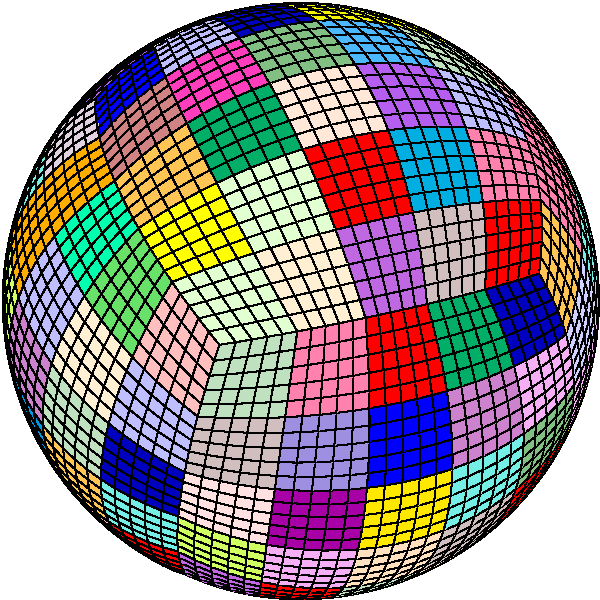
\includegraphics[width=0.45\textwidth]{figures/mpi_slices.pdf}  & 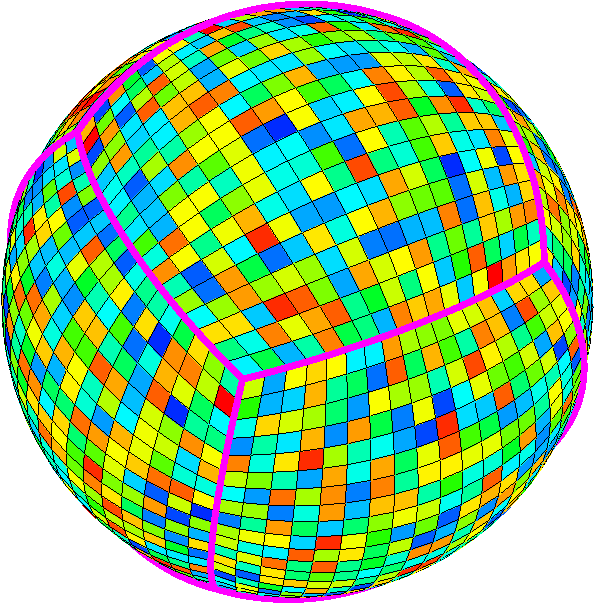
\includegraphics[width=0.45\textwidth]{figures/fullmesh_18.pdf} \\
%\end{tabular}
%\begin{minipage}[htp]{\textwidth}
%\begin{minipage}{0.5\textwidth}
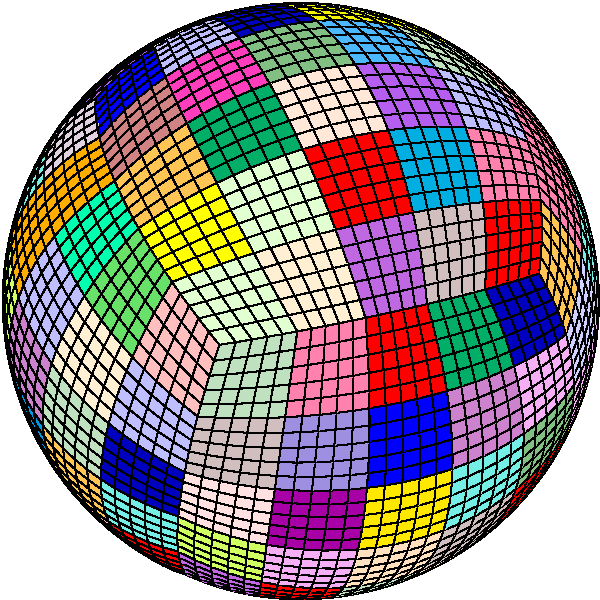
\includegraphics[width=0.45\textwidth]{figures/mpi_slices.pdf}
%\end{minipage}
\hfill
%\begin{minipage}[htp]{0.5\textwidth}
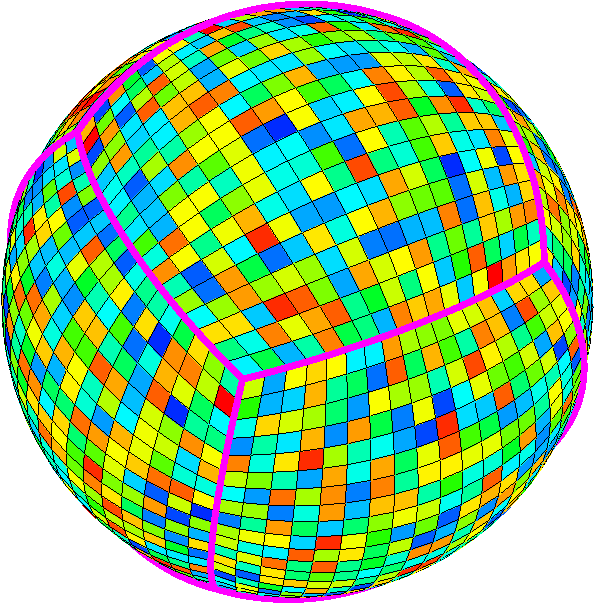
\includegraphics[width=0.45\textwidth]{figures/fullmesh_18.pdf}\\
%\end{minipage}
%\end{minipage}
\end{center}
\caption{Each of the 6~chunks that constitutes the cubed sphere is subdivided
in terms of $n^{2}$~slices of elements, where $n\ge1$ is a positive
integer, for a total of $6\times n^{2}$ slices (and therefore processors).
The figure on the left shows a mesh that is divided in terms of $6\times5^{2}=150$
slices as indicated by the various colors. In this cartoon, each slice
contains $5\times5=25$ spectral elements at the Earth's surface.
The figure on the right shows a mesh that is divided over $6\times18^{2}=1944$
processors as indicated by the various colors. Regional simulations
can be accommodated by using only 1, 2 or 3 chunks of the cubed sphere.
One-chunk simulations may involve a mesh with lateral dimensions smaller
than~$90^{\circ}$, thereby accommodating smaller-scale simulations. }
\label{figure:mpi_slices}
\end{figure}


To run the mesher for a global simulation, the following parameters
need to be set in the \texttt{Par\_file} (the list below might be slightly obsolete or incomplete; for an up-to-date
version, see comments in the default \texttt{Par\_file} located in directory \texttt{DATA}:


\begin{description}
\item [{\texttt{SIMULATION\_TYPE}}] is set to 1 for forward simulations,
2 for adjoint simulations for sources (see Section \ref{sec:Adjoint-simulation-sources})
and 3 for kernel simulations (see Section \ref{sec:Finite-Frequency-Kernels}).
%
\item [{\texttt{SAVE\_FORWARD}}] is only set to \texttt{.true.} for a forward
simulation with the last frame of the simulation saved, as part of
the finite-frequency kernel calculations (see Section \ref{sec:Finite-Frequency-Kernels}).
For a regular forward simulation, leave \texttt{SIMULATION\_TYPE}
and \texttt{SAVE\_FORWARD} at their default values.
%
\item [{\texttt{NCHUNKS}}] must be set to 6 for global simulations.
%
\item [{\texttt{ANGULAR\_WIDTH\_XI\_IN\_DEGREES}}] Not needed for a global
simulation. (See Chapter~\ref{cha:Regional-Simulations} for regional simulations.)
%
\item [{\texttt{ANGULAR\_WIDTH\_ETA\_IN\_DEGREES}}] Not needed for a global
simulation. (See Chapter~\ref{cha:Regional-Simulations} for regional simulations.)
%
\item [{\texttt{CENTER\_LATITUDE\_IN\_DEGREES}}] Not needed for a global
simulation. (See Chapter~\ref{cha:Regional-Simulations} for regional simulations.)
%
\item [{\texttt{CENTER\_LONGITUDE\_IN\_DEGREES}}] Not needed for a global
simulation. (See Chapter~\ref{cha:Regional-Simulations} for regional simulations.)
%
\item [{\texttt{GAMMA\_ROTATION\_AZIMUTH}}] Not needed for a global simulation.
(See Chapter~\ref{cha:Regional-Simulations}  for regional simulations.)
%
\item [{\texttt{NEX\_XI}}] The number of spectral elements along one side of a
chunk in the cubed sphere (see Figure~\ref{figure:mpi_slices});
this number \textit{must} be a multiple of 16 and 8~$\times$~a
multiple of $\nprocxi$ defined below. We do not recommend using $\nexxi$
less than 64 because the curvature of the Earth cannot be honored
if one uses too few elements, and distorted elements can lead to inaccurate
and unstable simulations, i.e., smaller values of $\nexxi$ are likely
to result in spectral elements with a negative Jacobian, in which
case the mesher will exit with an error message. Table~\ref{table:nex}
summarizes various suitable choices for $\nexxi$ and the related
values of $\nprocxi$. Based upon benchmarks against semi-analytical
normal-mode synthetic seismograms, \citet{KoTr02a,KoTr02b} determined
that a $\nexxi=256$ run is accurate to a shortest period of roughly
17~s. Therefore, since accuracy is determined by the number of grid
points per shortest wavelength, for any particular value of $\nexxi$
the simulation will be accurate to a shortest period determined approximately
by
\begin{equation}
\mbox{shortest period (s)}\simeq(256/\nexxi)\times17.\label{eq:shortest_period}
\end{equation}
 The number of grid points in each orthogonal direction of the reference
element, i.e., the number of Gauss-Lobatto-Legendre points, is determined
by \texttt{NGLLX} in the \texttt{constants.h} file. In the globe we
use $\mbox{\texttt{NGLLX}}=5$, for a total of $5^{3}=125$ points
per elements. We suggest not to change this value.
%
\item [{\texttt{NEX\_ETA}}] For global simulations $\nexeta$ must be set to the same value as $\nexxi$.
%
\item [{\texttt{NPROC\_XI}}] The number of processors or slices along one chunk
of the cubed sphere (see Figure~\ref{figure:mpi_slices}); we must
have $\nexxi=8\times c\times\nprocxi$, where $c\ge1$ is a positive
integer. See Table~\ref{table:nex} for various suitable choices.
%
\item [{\texttt{NPROC\_ETA}}] For global simulations $\nproceta$ must be set to the same value as $\nprocxi$.
%
\item [{\texttt{MODEL}}] Must be set to one of the following:
%
\item [{\textmd{1D~models~with~real~structure:}}]~
%%
\begin{description}
\item [{\texttt{1D\_isotropic\_prem}}] Isotropic version of the spherically
symmetric Preliminary Reference Earth Model (PREM) \citep{DzAn81}.
%
\item [{\texttt{1D\_transversely\_isotropic\_prem}}] Transversely isotropic version of PREM.
%
\item [{\texttt{1D\_iasp91}}] Spherically symmetric isotropic IASP91 model \citep{KeEn91}.
%
\item [{\texttt{1D\_1066a}}] Spherically symmetric earth model 1066A \citep{gilbertdziewonski1975}.
When \texttt{\small ATTENTUATION} is on, it uses an unpublished 1D
attenuation model from Scripps.
%
\item [{\texttt{1D\_ak135f\_no\_mud}}] Spherically symmetric isotropic AK135 model
\citep{KeEnBu95} modified to use the density and Q attenuation models of \cite{MoKe95}.
That modified model is traditionally called AK135-F,
see \url{http://rses.anu.edu.au/seismology/ak135/ak135f.html} for more details.
As we do not want to use the 300~m-thick mud layer from that model nor the ocean layer,
above the d120 discontinuity we switch back to the classical AK135 model of \cite{KeEnBu95},
i.e., we use AK135-F below and AK135 above.
%
\item [{\texttt{1D\_ref}}] A 1D Earth model developed by \citet{KuDzEk06}.
This model is the 1D background model for the 3D models s362ani, s362wmani,
s362ani\_prem, and s29ea.
%
\item [{\texttt{1D\_CCREM}}] A 1D Earth model developed by \citet{Ma2021} called CCREM:
a new reference Earth model from the global coda-correlation wavefield.
%
\item [{\texttt{Ishii}}] Combines the 1D transversely isotropic PREM with the anisotropic inner core model defined by \citet{Ishii2002}.
%
\end{description}
%%
for Mars:
\begin{description}
%
\item [{\texttt{1D\_Sohl}}] 1D Mars model developed by \citet{Sohl1997}.
This model is model A, mostly constrained by geophysical moment of inertia.
%
\item [{\texttt{1D\_case65TAY}}] 1D Mars reference model developed by \citet{Plesa2021}.
The model is the 1D reference model for case 65 with a compositional model by Taylor.
%
\end{description}
%%
for Moon:
\begin{description}
%
\item [{\texttt{VPREMOON}}] 1D Moon model developed by \citet{Garcia2011}.
Uses modified seismic model, starting from table 6 (left side, not geodesic model) with
velocity values for outer core and solid inner core based on \citet{Weber2011}
%
\end{description}
%%
\end{description}
For historical reasons and to provide benchmarks against normal-mode
synthetics, the mesher accommodates versions of various 1D models
with a single crustal layer with the properties of the original upper
crust. These `one-crust' models are:
\begin{verbatim}
  1D_isotropic_prem_onecrust
  1D_transversely_isotropic_prem_onecrust
  1D_iasp91_onecrust
  1D_1066a_onecrust
  1D_ak135f_no_mud_onecrust
\end{verbatim}

\begin{description}
\item [{\textmd{Fully~3D~models:}}]~
%%
\begin{description}
\item [{\texttt{transversely\_isotropic\_prem\_plus\_3D\_crust\_2.0}}] This
model has CRUST2.0 \citep{BaLaMa00} on top of a transversely isotropic
PREM. We first extrapolate PREM mantle velocity up to the surface,
then overwrite the model with CRUST2.0
%
\item [{\texttt{s20rts}}] By default, the code uses 3D mantle model S20RTS
\citep{RiVaWo99} and 3D crustal model Crust2.0 \citep{BaLaMa00}.
Note that S20RTS uses transversely isotropic PREM as a background
model, and that we use the PREM radial attenuation model when \texttt{ATTENUATION}
is incorporated. See Chapter~\ref{cha:-Changing-the} for a discussion
on how to change 3D models.
%
\item [{\texttt{s40rts}}] A global 3D mantle model \citep{RiDeVaWo11} succeeding S20RTS
with a higher resolution.
S40RTS uses transversely isotropic PREM as a backgroun
model and the 3D crustal model Crust2.0 \citep{BaLaMa00}.
We use the PREM radial attenuation model when \texttt{ATTENUATION}
is incorporated.
%
\item [{\texttt{s362ani}}] A global shear-wave speed
model developed by \citet{KuDzEk06}. In this model, radial anisotropy
is confined to the uppermost mantle. The model (and the corresponding
mesh) incorporate tomography on the 650~km and 410~km
discontinuities in the 1D reference model REF.
%
\item [{\texttt{s362wmani}}] A version of S362ANI with
anisotropy allowed throughout the mantle.
%
\item [{\texttt{s362ani\_prem}}] A version of S362ANI
calculated using PREM as the 1D reference model.
%
\item [{\texttt{s29ea}}] A global model with higher
resolution in the upper mantle beneath Eurasia calculated using REF
as the 1D reference model.
%
\item [{\texttt{3D\_anisotropic}}] See Chapter~\ref{cha:-Changing-the}
for a discussion on how to specify your own 3D anisotropic model.
%
\item [{\texttt{3D\_attenuation}}] See Chapter~\ref{cha:-Changing-the}
for a discussion on how to specify your own 3D attenuation model.
%
\item [{\texttt{PPM}}] For a user-specified 3D model (Point-Profile-Model)
given as ASCII-table, specifying Vs-perturbations
with respect to PREM. See Chapter~\ref{cha:-Changing-the}
for a discussion on how to specify your own 3D model.
%
\item [{\texttt{full\_sh}}] For a user-specified, transversely isotropic 3D model given in spherical harmonics. Coefficients for the crustal model (up to degree 40) are stored in files named \texttt{C**.dat} and \texttt{MOHO.dat}, coefficients for the mantle model (up to degree 20) are stored in files named \texttt{M**.dat}.\\
All model files reside in directory \texttt{DATA/full\_sphericalharmonic\_model/}. Note that to use the crustal model, one has to set the crustal type value \texttt{ITYPE\_CRUSTAL\_MODEL = ICRUST\_CRUST\_SH} in file \texttt{setup/constants.h}. This crustal model can be transversely isotropic as well.
%
\item [{\texttt{sgloberani\_iso}}] By default, the code uses 3D {\it isotropic} mantle model SGLOBE-rani \citep{Chang2015} and the 3D crustal model includes perturbations from Crust2.0 \citep{BaLaMa00} as discussed in \citep{Chang2015}. The model is parametrised horizontally in spherical harmonics up to \texttt{lmax=35} and with 21 depth splines for the radial direction. Note that SGLOBE-rani uses transversely isotropic PREM as a background model, and that we use the PREM radial attenuation model when \texttt{ATTENUATION} is incorporated.
%
\item [{\texttt{sgloberani\_aniso}}] By default, the code uses 3D {\it anisotropic} mantle model SGLOBE-rani \citep{Chang2015} and the 3D crustal model includes perturbations from Crust2.0 \citep{BaLaMa00} as discussed in \citep{Chang2015}. Note that SGLOBE-rani uses transversely isotropic PREM as a background model, and that we use the PREM radial attenuation model when \texttt{ATTENUATION} is incorporated.
%
\item [{\texttt{SPiRaL}}] A multiresolution global tomography model of seismic wave speeds
and radial anisotropy variations in the crust and mantle developed by \citet{Simmons2021}.
Please see folder \texttt{DATA/spiral1.4} for further information on how to install the corresponding model files.
%
\item [{\texttt{GLAD\_bkmns}}] A Block Mantle \& Spherical Harmonics (BKMNS) expansion model developed by \citet{Ciardelli2021}
for global crust/mantle 3D models GLAD-M25 and GLAD-M15.
Please see folder \texttt{DATA/gladm25} for further information on how to install the corresponding model files.
%
\end{description}
%%
for Mars:
\begin{description}
%
\item [{\texttt{1D\_Sohl\_3d\_crust}}] This model adds a 3D crust on top of the 1D Mars model developed by \citet{Sohl1997}.
The crustal model is defined by the files in folder \texttt{DATA/crustmaps/marscrust*.cmap}
%
\item [{\texttt{1D\_case65TAY\_3d\_crust}}] This model adds a 3D crust on top of the 1D Mars model developed by \citet{Plesa2021}.
The crustal model is defined by the files in folder \texttt{DATA/crustmaps/marscrust*.cmap}
%
\end{description}

%%
\item [{\textmd{Note:}}]~\\
When a 3D mantle model is chosen in \texttt{Par\_file}, the simulations are performed together with the associated 3D crustal model. For example, model \texttt{s362ani} would use by default crustal model Crust2.0.
To select the higher-resolution Crust1.0 crustal model instead, one can append it as an ending to the model name, i.e., \texttt{***<3D mantle>***\_crust1.0}, as for example \texttt{s362ani\_crust1.0}. In a similar way, various 3D crustal models defined such as \texttt{***\_crust1.0}, \texttt{***\_crust2.0}, \texttt{***\_crustmaps}, \texttt{***\_epcrust}, \texttt{***\_eucrust}, \texttt{***\_crustSH}, \texttt{***\_sglobecrust} and \texttt{***\_crustSPiRaL} can be combined with different mantle models.
Regional higher-resolution models, such as the European crustal models EPcrust \citep{Molinari2011} and EUCrust-07 \citep{EUCrust07} are embedded by default into the global crustal model Crust1.0.

It is also possible to run simulations using a 3D mantle model with a 1D crustal model on top. This can be done by setting the model in \texttt{Par\_file} to \texttt{***<3D mantle>***\_1Dcrust}, e.g., \texttt{s20rts\_1Dcrust, s362ani\_1Dcrust}, etc. In this case, the 1D crustal model will be the one that is used in the 3D mantle model as a reference model (e.g., transversely isotropic PREM for s20rts, REF for s362ani, etc.).

Currently, the only anisotropic inner core model implemented is the one defined by \citet{Ishii2002}. To use this anisotropic inner core model, one can append the ending \texttt{***<3D mantle>***\_AIC} to the mantle model name. With the above crustal ending, as an example one could use \texttt{s362ani\_crust1.0\_AIC}.
%
\item [{\texttt{OCEANS}}] Set to \texttt{.true.} if the effect of the oceans
on seismic wave propagation should be incorporated based upon the
approximate treatment discussed in \citet{KoTr02b}. This feature
is inexpensive from a numerical perspective, both in terms of memory
requirements and CPU time. This approximation is accurate at periods
of roughly 20~s and longer. At shorter periods the effect of water
phases/reverberations is not taken into account, even when the flag
is on.
%
\item [{\texttt{ELLIPTICITY}}] Set to \texttt{.true.} if the mesh should
make the Earth model elliptical in shape according to Clairaut's equation
\citep{DaTr98}. This feature adds no cost to the simulation.
After adding ellipticity, the mesh becomes elliptical and thus geocentric and geodetic/geographic latitudes and colatitudes differ (longitudes are unchanged).
%
From \cite{DaTr98}: "Spherically-symmetric Earth models all have the same hydrostatic surface ellipticity 1/299.8. This is 0.5 percent smaller than observed flattening of best-fitting ellipsoid 1/298.3. The discrepancy is referred to as the "excess equatorial bulge of the Earth", an early discovery of artificial satellite geodesy."
%
From Paul Melchior, IUGG General Assembly, Vienna, Austria, August 1991 Union lecture, available at www.agu.org/books: "It turns out that the spheroidal models constructed on the basis of the spherically-symmetric models (PREM, 1066A) by using the Clairaut differential equation to calculate the flattening
in function of the radius vector imply hydrostaticity. These have surface ellipticity 1/299.8 and
a corresponding dynamical flattening of .0033 (PREM). The actual ellipticty of the Earth for a best-fitting ellipsoid is 1/298.3 with a corresponding dynamical flattening of .0034."

Thus, flattening f = 1/299.8 is what is used in SPECFEM3D\_GLOBE, as it should. And eccentricity squared $e^2 = 1 - (1-f)^2 = 1 - (1 - 1/299.8)^2 = 0.00665998813529$, and the correction factor used in the code to convert geographic latitudes to geocentric is $1 - e^2 = (1-f)^2 = (1 - 1/299.8)^2 = 0.9933400118647$.
%
As a comparison, the classical World Geodetic System reference ellipsoid WGS 84 (see e.g. \url{http://en.wikipedia.org/wiki/World_Geodetic_System}) has $f = 1/298.2572236$.

For Mars, a flattening factor 1/169.8 is used (based on Smith et al. 1999, Science, 284). For Moon, a flattening factor 1/901.0 is currently taken. These values can be modified in file \texttt{setup/constants.h}.

%
\item [{\texttt{TOPOGRAPHY}}] Set to \texttt{.true.} if topography and
bathymetry should be incorporated based upon model ETOPO4 \citep{Etopo5}.
This feature adds no cost to the simulation.
If you want to use other topographic models, please see folder \texttt{DATA/topo\_bathy/} for further infos and change the name of the topographic model to use in file \texttt{setup/constants.h} before re-compiling the code.
%
\item [{\texttt{GRAVITY}}] Set to \texttt{.true.} if self-gravitation should
be incorporated in the Cowling approximation \citep{KoTr02b,DaTr98}.
Turning this feature on is relatively inexpensive, both from the perspective
of memory requirements as well as in terms of computational speed.
%
\item [{\texttt{ROTATION}}] Set to \texttt{.true.} if the Coriolis effect
should be incorporated. Turning this feature on is relatively cheap
numerically.
%
\item [{\texttt{ATTENUATION}}] Set to \texttt{.true.} if attenuation should
be incorporated. Turning this feature on increases the memory requirements
significantly (roughly by a factor of~2), and is numerically fairly
expensive. Of course for realistic simulations this flag should be
turned on. See \citet{KoTr99,KoTr02a} for a discussion on the implementation
of attenuation based upon standard linear solids.
%
\item [{\texttt{ABSORBING\_CONDITIONS}}] Set to \texttt{.false.} for global
simulations. See Chapter~\ref{cha:Regional-Simulations} for regional
simulations.
%
\item [{\texttt{RECORD\_LENGTH\_IN\_MINUTES}}] Choose the desired record
length of the synthetic seismograms (in minutes). This controls the
length of the numerical simulation, i.e., twice the record length
requires twice as much CPU time. This feature is not used at the time
of meshing but is required for the solver, i.e., you may change this
parameter after running the mesher.
%
\item [{\texttt{PARTIAL\_PHYS\_DISPERSION\_ONLY} or \texttt{UNDO\_ATTENUATION}}] To undo attenuation for sensitivity kernel calculations or forward runs with \texttt{SAVE\_FORWARD}
use one (and only one) of the two flags below. \texttt{UNDO\_ATTENUATION} is much better (it is exact) and is simpler to use
but it requires a significant amount of disk space for temporary storage. It has the advantage of requiring only two simulations for adjoint tomography instead
of three in the case of \texttt{PARTIAL\_PHYS\_DISPERSION\_ONLY}, i.e. for adjoint tomography it is globally significantly less expensive (each run is slightly more
expensive, but only two runs are needed instead of three).\\
When using \texttt{PARTIAL\_PHYS\_DISPERSION\_ONLY}, to make the approximation reasonably OK you need to take the following steps:
\begin{enumerate}
\item[1/] To calculate synthetic seismograms, do a forward simulation with full attenuation for the model of interest. The goal is to get synthetics that match the data as closely as possible.
\item[2a/] Make measurements and produce adjoint sources by comparing the resulting synthetics with the data. In the simplest case of a cross-correlation traveltime measurement, use the time-reversed synthetic in the window of interest as the adjoint source.
\item[2b/] Do a second forward calculation with \texttt{PARTIAL\_PHYS\_DISPERSION\_ONLY = .true.} and save the last snapshot.
\item[3/] Do an adjoint calculation using the adjoint source calculated in 1/, the forward wavefield reconstructed based on 2b/, use \texttt{PARTIAL\_PHYS\_DISPERSION\_ONLY = .true.} for the adjoint wavefield, and save the kernel.
\end{enumerate}
Thus the kernel calculation uses \texttt{PARTIAL\_PHYS\_DISPERSION\_ONLY = .true.} for both the forward and the adjoint wavefields. This is in the spirit of the banana-donut kernels. But the data that are assimilated are based on the full 3D synthetic with attenuation.\\
%
Another, equivalent way of explaining it is:
\begin{enumerate}
\item[1/] Calculate synthetics with full attenuation for the current model. Compare these to the data and measure frequency-dependent traveltime anomalies $\Delta \tau(\omega)$, e.g.. based upon multi-tapering.
\item[2/] Calculate synthetics with \texttt{PARTIAL\_PHYS\_DISPERSION\_ONLY = .true.} and construct adjoint sources by combining the seismograms from this run with the measurements from 1/. So in the expressions for the multi-taper adjoint source you use the measurements from 1/, but synthetics calculated with \texttt{PARTIAL\_PHYS\_DISPERSION\_ONLY = .true.}.
\item[3/] Construct a kernel by calculating an adjoint wavefield based on the sources constructed in 2/ and convolving it with a forward wavefield with \texttt{PARTIAL\_PHYS\_DISPERSION\_ONLY = .true.}. Again, both the forward and adjoint calculations use \texttt{PARTIAL\_PHYS\_DISPERSION\_ONLY = .true.}.
\end{enumerate}
Note that if you replace multi-taper measurements with cross-correlation measurements you will measure a cross-correlation traveltime anomaly in 1/, i.e., some delay time $\Delta T$. Then you would calculate an adjoint wavefield with \texttt{PARTIAL\_PHYS\_DISPERSION\_ONLY = .true.} and use the resulting time-reversed seismograms weighted by $\Delta T$ as the adjoint source. This wavefield interacts with a forward wavefield calculated with \texttt{PARTIAL\_PHYS\_DISPERSION\_ONLY = .true.}.
If $\Delta T=1$ one gets a banana-donut kernel, i.e., a kernel for the case in which there are no observed seismograms (no data), as explained for instance on page 5 of \cite{ZhLiTr11}.
%
\item [{\texttt{MOVIE\_SURFACE}}] Set to \texttt{.false.}, unless you want
to create a movie of seismic wave propagation on the Earth's surface.
Turning this option on generates large output files. See Section \ref{sec:Movies}
for a discussion on the generation of movies. This feature is not
used at the time of meshing but is relevant for the solver.
%
\item [{\texttt{MOVIE\_VOLUME}}] Set to \texttt{.false.}, unless you want
to create a movie of seismic wave propagation in the Earth's interior.
Turning this option on generates huge output files. See Section \ref{sec:Movies}
for a discussion on the generation of movies. This feature is not
used at the time of meshing but is relevant for the solver.
%
\item [{\texttt{NTSTEP\_BETWEEN\_FRAMES}}] Determines the number of timesteps
between movie frames. Typically you want to save a snapshot every
100 timesteps. The smaller you make this number the more output will
be generated! See Section \ref{sec:Movies} for a discussion on the
generation of movies. This feature is not used at the time of meshing
but is relevant for the solver.
%
\item [{\texttt{HDUR\_MOVIE}}] determines the half duration of the source
time function for the movie simulations. When this parameter is set
to be 0, a default half duration that corresponds to the accuracy
of the simulation is provided.
%
\item [{\texttt{SAVE\_MESH\_FILES}}] Set this flag to \texttt{.true}\texttt{\small .}
to save AVS \urlwithparentheses{http://www.avs.com}, OpenDX \urlwithparentheses{http://www.opendx.org}, or ParaView \urlwithparentheses{http://www.paraview.org}
mesh files for subsequent viewing. Turning the flag on generates large
(distributed) files in the \texttt{LOCAL\_PATH} directory. See Section~\ref{sec:Meshes}
for a discussion of mesh viewing features.
%
\item [{\texttt{NUMBER\_OF\_RUNS}}] On machines with a run-time limit,
for instance for a batch/queue system, a simulation may need to be
completed in stages. This option allows you to select the number of
stages in which the simulation will be completed (1, 2 or 3). Choose
1 for a run without restart files. This feature is not used at the
time of meshing but is required for the solver. At the end of the
first or second stage of a multi-stage simulation, large files are
written to the file system to save the current state of the simulation.
This state is read back from the file system at the beginning of the
next stage of the multi-stage run. Reading and writing the states
can be very time consuming depending on the nature of the network
and the file system (in this case writing to the local file system,
i.e., the disk on a node, is preferable).
%
\item [{\texttt{NUMBER\_OF\_THIS\_RUN}}] If you choose to perform the run
in stages, you need to tell the solver what stage run to perform.
This feature is not used at the time of meshing but is required for
the solver.
%
\item [{\texttt{LOCAL\_PATH}}] Directory in which the databases generated
by the mesher will be written. Generally one uses a directory on the
local disk of the compute nodes, although on some machines these databases
are written on a parallel (global) file system (see also the earlier
discussion of the \texttt{LOCAL\_PATH\_IS\_ALSO\_GLOBAL} flag in Chapter~\ref{cha:Getting-Started}).
The mesher generates the necessary databases in parallel, one set
for each of the $6\times\nprocxi^{2}$ slices that constitutes the
mesh (see Figure~\ref{figure:mpi_slices}). After the mesher finishes,
you can log in to one of the compute nodes and view the contents of
the \texttt{LOCAL\_PATH} directory to see the (many) files generated
by the mesher.
%
\item [{\texttt{NTSTEP\_BETWEEN\_OUTPUT\_INFO}}] This parameter specifies
the interval at which basic information about a run is written to
the file system (\texttt{timestamp{*}} files in the \texttt{OUTPUT\_FILES}
directory). If you have access to a fast machine, set \texttt{NTSTEP\_BETWEEN\_OUTPUT\_INFO}
to a relatively high value (e.g., at least 100, or even 1000 or more)
to avoid writing output text files too often. This feature is not
used at the time of meshing. One can set this parameter to a larger
value than the number of time steps to avoid writing output during
the run.
%
\item [{\texttt{NTSTEP\_BETWEEN\_OUTPUT\_SEISMOS}}] This parameter specifies
the interval at which synthetic seismograms are written in the \texttt{LOCAL\_PATH}
directory. The seismograms can be created in three different formats
by setting the parameters \texttt{OUTPUT\_SEISMOS\_ASCII\_TEXT}, \texttt{OUTPUT\_SEISMOS\_SAC\_ALPHANUM}
and \texttt{OUTPUT\_SEI-}~\\
\texttt{SMOS\_SAC\_BINARY}. One can choose any combination of these
parameters (details on the formats follow in the description of each
parameter). SAC \urlwithparentheses{http://www.iris.edu/software/sac/} is a signal-processing software
package. If a run crashes, you may still find usable (but shorter
than requested) seismograms in this directory. On a fast machine set
\texttt{NTSTEP\_BETWEEN\_OUTPUT\_SEISMOS} to a relatively high value
to avoid writing to the seismograms too often. This feature is not
used at the time of meshing.
%
\item [{\texttt{NTSTEP\_BETWEEN\_READ\_ADJSRC}}] The number of adjoint
sources read in each time for an adjoint simulation.
%
\item [{\texttt{USE\_FORCE\_POINT\_SOURCE}}] Turn this flag on to use a
(tilted) \texttt{FORCESOLUTION} force point source instead of a \texttt{CMTSOLUTION}
moment-tensor source. When the force source does not fall exactly
at a grid point, the solver interpolates the force between grid points
using Lagrange interpolants. This option can be useful for vertical force, normal
force, tilted force, impact force, etc. Note that in the \texttt{FORCESOLUTION}
file, you will need to edit the East, North and vertical components
of an arbitrary (not necessarily unitary, the code will normalize it automatically) direction vector of the force vector;
thus refer to Appendix~\ref{cha:Reference-Frame-Convention} for the orientation
of the reference frame. This vector is made unitary internally in
the solver and thus only its direction matters here; its norm is ignored
and the norm of the force used is the factor force source times the
source time function.
%
\item [{\texttt{OUTPUT\_SEISMOS\_ASCII\_TEXT}}] Set this flag to \texttt{.true.}
if you want to have the synthetic seismograms written in two-column
ASCII format (the first column contains time in seconds and the second
column the displacement in meters of the recorded signal, no header
information). Files will be named with extension \texttt{.ascii}, e.g., \texttt{NT.STA.?X?.sem.ascii}
where NT and STA are the network and station codes given in \texttt{STATIONS} file, and \texttt{?X?} is the channel code (see Appendix~\ref{cha:channel-codes}).
%
\item [{\texttt{OUTPUT\_SEISMOS\_SAC\_ALPHANUM}}] Set this flag to \texttt{.true.}
if you want to have the synthetic seismograms written in alphanumeric
(human readable) SAC format, which includes header information on
the source and receiver parameters (e.g., source/receiver coordinates,
station name, etc., see Appendix~\ref{cha:SAC-headers}). For details on the format, please check the SAC webpage \urlwithparentheses{http://www.iris.edu/software/sac/}. Files will be named with extension \texttt{.sacan}.
%
\item [{\texttt{OUTPUT\_SEISMOS\_SAC\_BINARY}}] Set this flag to \texttt{.true.}
if you want to have the synthetic seismograms written in binary SAC
format. The header information included is the same as for the alphanumeric
SAC format (see Appendix~\ref{cha:SAC-headers}). Using this format requires the least disk space, which may be particulary important if you have a large number of stations.
For details on the binary format please also check the SAC webpage \urlwithparentheses{http://www.iris.edu/software/sac/} and Appendix~\ref{cha:SAC-headers}. Files will be named with extension \texttt{.sac}.
%
\item [{\texttt{ROTATE\_SEISMOGRAMS\_RT}}] Set this flag to \texttt{.true.}
if you want to have radial (R) and transverse (T) horizontal components
of the synthetic seismograms (default is \texttt{.false.} $\rightarrow$
East (E) and North (N) components).
%
\item [{\texttt{WRITE\_SEISMOGRAMS\_BY\_MAIN}}] Set this flag to \texttt{.true.}
if you want to have all the seismograms written by the main process (no
need to collect them on the nodes after the run).
%
\item [{\texttt{SAVE\_ALL\_SEISMOS\_IN\_ONE\_FILE}}] Set this flag to \texttt{.true.}
if you want to have all the seismograms saved in one large combined
file instead of one file per seismogram to avoid overloading shared
non-local file systems such as GPFS for instance.
%
\item [{\texttt{USE\_BINARY\_FOR\_LARGE\_FILE}}] Set this flag to \texttt{.true.}
if you want to use binary instead of ASCII for that large file (not
used if SAVE\_ALL\_SEISMOS\_IN \_ONE\_FILE = .false.)
%
\item [{\texttt{RECEIVERS\_CAN\_BE\_BURIED}}] This flag accommodates stations
with instruments that are buried, i.e., the solver will calculate
seismograms at the burial depth specified in the \texttt{STATIONS}
file. This feature is not used at the time of meshing.
%
\item [{\texttt{PRINT\_SOURCE\_TIME\_FUNCTION}}] Turn this flag on to print
information about the source time function in the file \texttt{OUTPUT\_FILES/plot\_source\_time\_function.txt}.
This feature is not used at the time of meshing.
%
\item [{\texttt{NUMBER\_OF\_SIMULTANEOUS\_RUNS}}] adds the ability to run several calculations (several earthquakes)
in an embarrassingly-parallel fashion from within the same run;
this can be useful when using a very large supercomputer to compute
many earthquakes in a catalog, in which case it can be better from
a batch job submission point of view to start fewer and much larger jobs,
each of them computing several earthquakes in parallel.

To turn that option on, set parameter NUMBER\_OF\_SIMULTANEOUS\_RUNS to a value greater than 1.
To implement that, we create NUMBER\_OF\_SIMULTANEOUS\_RUNS MPI sub-communicators,
each of them being labeled "my\_local\_mpi\_comm\_world", and we use them
in all the routines in "src/shared/parallel.f90", except in MPI\_ABORT() because in that case
we need to kill the entire run.

When that option is on, of course the number of processor cores used to start
the code in the batch system must be a multiple of NUMBER\_OF\_SIMULTANEOUS\_RUNS,
all the individual runs must use the same number of processor cores,
which as usual is NPROC in the Par\_file,
and thus the total number of processor cores to request from the batch system
should be NUMBER\_OF\_SIMULTANEOUS\_RUNS * NPROC.
All the runs to perform must be placed in directories called run0001, run0002, run0003 and so on
(with exactly four digits).

Imagine you have 10 independent calculations to do, each of them on 100 cores; you have three options:

1/ submit 10 jobs to the batch system

2/ submit a single job on 1000 cores to the batch, and in that script create a sub-array of jobs to start 10 jobs,
each running on 100 cores (see e.g. \url{http://www.schedmd.com/slurmdocs/job_array.html} )

3/ submit a single job on 1000 cores to the batch, start SPECFEM3D on 1000 cores, create 10 sub-communicators,
cd into one of 10 subdirectories (called e.g. run0001, run0002,... run0010) depending on the sub-communicator
your MPI rank belongs to, and run normally on 100 cores using that sub-communicator.

The option NUMBER\_OF\_SIMULTANEOUS\_RUNS implements 3/.

%
\item [{\texttt{BROADCAST\_SAME\_MESH\_AND\_MODEL}}]:
if we perform simultaneous runs in parallel, if only the source and receivers vary between these runs
but not the mesh nor the model (velocity and density) then we can also read the mesh and model files
from a single run in the beginning and broadcast them to all the others; for a large number of simultaneous
runs for instance when solving inverse problems iteratively this can DRASTICALLY reduce I/Os to disk in the solver
(by a factor equal to NUMBER\_OF\_SIMULTANEOUS\_RUNS), and reducing I/Os is crucial in the case of huge runs.
Thus, always set this option to .true. if the mesh and the model are the same for all simultaneous runs.
In that case there is no need to duplicate the mesh and model file database (the content of the DATABASES\_MPI
directories) in each of the run0001, run0002,... directories, it is sufficient to have one in run0001
and the code will broadcast it to the others).
%
\item [{\texttt{USE\_FAILSAFE\_MECHANISM}}]:
if one or a few of these simultaneous runs fail, kill all the runs or let the others finish using a fail-safe mechanism
(in most cases, should be set to true).

TODO / future work to do: currently the BROADCAST\_SAME\_MESH\_AND\_MODEL option assumes to have the (main) mesh files in run0001/DATABASES\_MPI or run0001/OUTPUT\_FILES/DATABASES\_MPI. However, for adjoint runs you still need a DATABASES\_MPI folder in each of the sub-runs directories, e.g. run0002/DATABASES\_MPI, etc. to store the forward wavefields, kernels etc. of each sub-run. This would not be needed for forward simulations.

TODO / future work to do: the sensitivity kernel summing and smoothing tools in directory src/tomography are currently not ported to this new option to do many runs simultaneously, only the solver (src/specfem3d) is. Thus these tools should work, but in their current version will need to be run for each simulation result independently.
More precisely, the current kernel summing and smoothing routines work fine, with the exception that you need to move out the mesh files (and also the parameters). This works because these routines consider multiple runs by design. You simply have to provide them the directories where the kernels are.
\end{description}
%

\clearpage
\noindent \begin{center}
\label{table:nex}
\begin{longtable}{|c|c|c|c|c|c|c|c|c|c|c|c|}
\hline
%\nprocxi & processors & \multicolumn{10}{c|}{\nexxi}\tabularnewline
%% better readability w/ pandoc
{\texttt{NPROC\_XI}} & processors & \multicolumn{10}{c|}{{\texttt{NEX\_XI}}}\tabularnewline
\hline
\endhead
\hline
1 & 6 & 64 & 80 & 96 & 112 & 128 & 144 & 160 & 176 & 192 & 208\tabularnewline
\hline
2 & 24 & 64 & 80 & 96 & 112 & 128 & 144 & 160 & 176 & 192 & 208\tabularnewline
\hline
3 & 54 & 96 & 144 & 192 & 240 & 288 & 336 & 384 & 432 & 480 & 528\tabularnewline
\hline
4 & 96 & 64 & 96 & 128 & 160 & 192 & 224 & 256 & 288 & 320 & 352\tabularnewline
\hline
5 & 150 & 80 & 160 & 240 & 320 & 400 & 480 & 560 & 640 & 720 & 800\tabularnewline
\hline
6 & 216 & 96 & 144 & 192 & 240 & 288 & 336 & 384 & 432 & 480 & 528\tabularnewline
\hline
7 & 294 & 112 & 224 & 336 & 448 & 560 & 672 & 784 & 896 & 1008 & 1120\tabularnewline
\hline
8 & 384 & 64 & 128 & 192 & 256 & 320 & 384 & 448 & 512 & 576 & 640\tabularnewline
\hline
9 & 486 & 144 & 288 & 432 & 576 & 720 & 864 & 1008 & 1152 & 1296 & 1440\tabularnewline
\hline
10 & 600 & 80 & 160 & 240 & 320 & 400 & 480 & 560 & 640 & 720 & 800\tabularnewline
\hline
11 & 726 & 176 & 352 & 528 & 704 & 880 & 1056 & 1232 & 1408 & 1584 & 1760\tabularnewline
\hline
12 & 864 & 96 & 192 & 288 & 384 & 480 & 576 & 672 & 768 & 864 & 960\tabularnewline
\hline
13 & 1014 & 208 & 416 & 624 & 832 & 1040 & 1248 & 1456 & 1664 & 1872 & 2080\tabularnewline
\hline
14 & 1176 & 112 & 224 & 336 & 448 & 560 & 672 & 784 & 896 & 1008 & 1120\tabularnewline
\hline
15 & 1350 & 240 & 480 & 720 & 960 & 1200 & 1440 & 1680 & 1920 & 2160 & 2400\tabularnewline
\hline
16 & 1536 & 128 & 256 & 384 & 512 & 640 & 768 & 896 & 1024 & 1152 & 1280\tabularnewline
\hline
17 & 1734 & 272 & 544 & 816 & 1088 & 1360 & 1632 & 1904 & 2176 & 2448 & 2720\tabularnewline
\hline
18 & 1944 & 144 & 288 & 432 & 576 & 720 & 864 & 1008 & 1152 & 1296 & 1440\tabularnewline
\hline
19 & 2166 & 304 & 608 & 912 & 1216 & 1520 & 1824 & 2128 & 2432 & 2736 & 3040\tabularnewline
\hline
20 & 2400 & 160 & 320 & 480 & 640 & 800 & 960 & 1120 & 1280 & 1440 & 1600\tabularnewline
\hline
21 & 2646 & 336 & 672 & 1008 & 1344 & 1680 & 2016 & 2352 & 2688 & 3024 & 3360\tabularnewline
\hline
22 & 2904 & 176 & 352 & 528 & 704 & 880 & 1056 & 1232 & 1408 & 1584 & 1760\tabularnewline
\hline
23 & 3174 & 368 & 736 & 1104 & 1472 & 1840 & 2208 & 2576 & 2944 & 3312 & 3680\tabularnewline
\hline
24 & 3456 & 192 & 384 & 576 & 768 & 960 & 1152 & 1344 & 1536 & 1728 & 1920\tabularnewline
\hline
25 & 3750 & 400 & 800 & 1200 & 1600 & 2000 & 2400 & 2800 & 3200 & 3600 & 4000\tabularnewline
\hline
26 & 4056 & 208 & 416 & 624 & 832 & 1040 & 1248 & 1456 & 1664 & 1872 & 2080\tabularnewline
\hline
27 & 4374 & 432 & 864 & 1296 & 1728 & 2160 & 2592 & 3024 & 3456 & 3888 & 4320\tabularnewline
\hline
28 & 4704 & 224 & 448 & 672 & 896 & 1120 & 1344 & 1568 & 1792 & 2016 & 2240\tabularnewline
\hline
29 & 5046 & 464 & 928 & 1392 & 1856 & 2320 & 2784 & 3248 & 3712 & 4176 & 4640\tabularnewline
\hline
30 & 5400 & 240 & 480 & 720 & 960 & 1200 & 1440 & 1680 & 1920 & 2160 & 2400\tabularnewline
\hline
31 & 5766 & 496 & 992 & 1488 & 1984 & 2480 & 2976 & 3472 & 3968 & 4464 & 4960\tabularnewline
\hline
32 & 6144 & 256 & 512 & 768 & 1024 & 1280 & 1536 & 1792 & 2048 & 2304 & 2560\tabularnewline
\hline
33 & 6534 & 528 & 1056 & 1584 & 2112 & 2640 & 3168 & 3696 & 4224 & 4752 & 5280\tabularnewline
\hline
34 & 6936 & 272 & 544 & 816 & 1088 & 1360 & 1632 & 1904 & 2176 & 2448 & 2720\tabularnewline
\hline
35 & 7350 & 560 & 1120 & 1680 & 2240 & 2800 & 3360 & 3920 & 4480 & 5040 & 5600\tabularnewline
\hline
36 & 7776 & 288 & 576 & 864 & 1152 & 1440 & 1728 & 2016 & 2304 & 2592 & 2880\tabularnewline
\hline
37 & 8214 & 592 & 1184 & 1776 & 2368 & 2960 & 3552 & 4144 & 4736 & 5328 & 5920\tabularnewline
\hline
38 & 8664 & 304 & 608 & 912 & 1216 & 1520 & 1824 & 2128 & 2432 & 2736 & 3040\tabularnewline
\hline
39 & 9126 & 624 & 1248 & 1872 & 2496 & 3120 & 3744 & 4368 & 4992 & 5616 & 6240\tabularnewline
\hline
40 & 9600 & 320 & 640 & 960 & 1280 & 1600 & 1920 & 2240 & 2560 & 2880 & 3200\tabularnewline
\hline
41 & 10086 & 656 & 1312 & 1968 & 2624 & 3280 & 3936 & 4592 & 5248 & 5904 & 6560\tabularnewline
\hline
42 & 10584 & 336 & 672 & 1008 & 1344 & 1680 & 2016 & 2352 & 2688 & 3024 & 3360\tabularnewline
\hline
43 & 11094 & 688 & 1376 & 2064 & 2752 & 3440 & 4128 & 4816 & 5504 & 6192 & 6880\tabularnewline
\hline
44 & 11616 & 352 & 704 & 1056 & 1408 & 1760 & 2112 & 2464 & 2816 & 3168 & 3520\tabularnewline
\hline
45 & 12150 & 720 & 1440 & 2160 & 2880 & 3600 & 4320 & 5040 & 5760 & 6480 & 7200\tabularnewline
\hline
46 & 12696 & 368 & 736 & 1104 & 1472 & 1840 & 2208 & 2576 & 2944 & 3312 & 3680\tabularnewline
\hline
47 & 13254 & 752 & 1504 & 2256 & 3008 & 3760 & 4512 & 5264 & 6016 & 6768 & 7520\tabularnewline
\hline
48 & 13824 & 384 & 768 & 1152 & 1536 & 1920 & 2304 & 2688 & 3072 & 3456 & 3840\tabularnewline
\hline
49 & 14406 & 784 & 1568 & 2352 & 3136 & 3920 & 4704 & 5488 & 6272 & 7056 & 7840\tabularnewline
\hline
50 & 15000 & 400 & 800 & 1200 & 1600 & 2000 & 2400 & 2800 & 3200 & 3600 & 4000\tabularnewline
\hline
51 & 15606 & 816 & 1632 & 2448 & 3264 & 4080 & 4896 & 5712 & 6528 & 7344 & 8160\tabularnewline
\hline
52 & 16224 & 416 & 832 & 1248 & 1664 & 2080 & 2496 & 2912 & 3328 & 3744 & 4160\tabularnewline
\hline
53 & 16854 & 848 & 1696 & 2544 & 3392 & 4240 & 5088 & 5936 & 6784 & 7632 & 8480\tabularnewline
\hline
54 & 17496 & 432 & 864 & 1296 & 1728 & 2160 & 2592 & 3024 & 3456 & 3888 & 4320\tabularnewline
\hline
55 & 18150 & 880 & 1760 & 2640 & 3520 & 4400 & 5280 & 6160 & 7040 & 7920 & 8800\tabularnewline
\hline
56 & 18816 & 448 & 896 & 1344 & 1792 & 2240 & 2688 & 3136 & 3584 & 4032 & 4480\tabularnewline
\hline
57 & 19494 & 912 & 1824 & 2736 & 3648 & 4560 & 5472 & 6384 & 7296 & 8208 & 9120\tabularnewline
\hline
58 & 20184 & 464 & 928 & 1392 & 1856 & 2320 & 2784 & 3248 & 3712 & 4176 & 4640\tabularnewline
\hline
59 & 20886 & 944 & 1888 & 2832 & 3776 & 4720 & 5664 & 6608 & 7552 & 8496 & 9440\tabularnewline
\hline
60 & 21600 & 480 & 960 & 1440 & 1920 & 2400 & 2880 & 3360 & 3840 & 4320 & 4800\tabularnewline
\hline
61 & 22326 & 976 & 1952 & 2928 & 3904 & 4880 & 5856 & 6832 & 7808 & 8784 & 9760\tabularnewline
\hline
62 & 23064 & 496 & 992 & 1488 & 1984 & 2480 & 2976 & 3472 & 3968 & 4464 & 4960\tabularnewline
\hline
63 & 23814 & 1008 & 2016 & 3024 & 4032 & 5040 & 6048 & 7056 & 8064 & 9072 & 10080\tabularnewline
\hline
64 & 24576 & 512 & 1024 & 1536 & 2048 & 2560 & 3072 & 3584 & 4096 & 4608 & 5120\tabularnewline
\hline
65 & 25350 & 1040 & 2080 & 3120 & 4160 & 5200 & 6240 & 7280 & 8320 & 9360 & 10400\tabularnewline
\hline
66 & 26136 & 528 & 1056 & 1584 & 2112 & 2640 & 3168 & 3696 & 4224 & 4752 & 5280\tabularnewline
\hline
67 & 26934 & 1072 & 2144 & 3216 & 4288 & 5360 & 6432 & 7504 & 8576 & 9648 & 10720\tabularnewline
\hline
68 & 27744 & 544 & 1088 & 1632 & 2176 & 2720 & 3264 & 3808 & 4352 & 4896 & 5440\tabularnewline
\hline
69 & 28566 & 1104 & 2208 & 3312 & 4416 & 5520 & 6624 & 7728 & 8832 & 9936 & 11040\tabularnewline
\hline
70 & 29400 & 560 & 1120 & 1680 & 2240 & 2800 & 3360 & 3920 & 4480 & 5040 & 5600\tabularnewline
\hline
71 & 30246 & 1136 & 2272 & 3408 & 4544 & 5680 & 6816 & 7952 & 9088 & 10224 & 11360\tabularnewline
\hline
72 & 31104 & 576 & 1152 & 1728 & 2304 & 2880 & 3456 & 4032 & 4608 & 5184 & 5760\tabularnewline
\hline
73 & 31974 & 1168 & 2336 & 3504 & 4672 & 5840 & 7008 & 8176 & 9344 & 10512 & 11680\tabularnewline
\hline
74 & 32856 & 592 & 1184 & 1776 & 2368 & 2960 & 3552 & 4144 & 4736 & 5328 & 5920\tabularnewline
\hline
75 & 33750 & 1200 & 2400 & 3600 & 4800 & 6000 & 7200 & 8400 & 9600 & 10800 & 12000\tabularnewline
\hline
76 & 34656 & 608 & 1216 & 1824 & 2432 & 3040 & 3648 & 4256 & 4864 & 5472 & 6080\tabularnewline
\hline
77 & 35574 & 1232 & 2464 & 3696 & 4928 & 6160 & 7392 & 8624 & 9856 & 11088 & 12320\tabularnewline
\hline
78 & 36504 & 624 & 1248 & 1872 & 2496 & 3120 & 3744 & 4368 & 4992 & 5616 & 6240\tabularnewline
\hline
79 & 37446 & 1264 & 2528 & 3792 & 5056 & 6320 & 7584 & 8848 & 10112 & 11376 & 12640\tabularnewline
\hline
80 & 38400 & 640 & 1280 & 1920 & 2560 & 3200 & 3840 & 4480 & 5120 & 5760 & 6400\tabularnewline
\hline
81 & 39366 & 1296 & 2592 & 3888 & 5184 & 6480 & 7776 & 9072 & 10368 & 11664 & 12960\tabularnewline
\hline
82 & 40344 & 656 & 1312 & 1968 & 2624 & 3280 & 3936 & 4592 & 5248 & 5904 & 6560\tabularnewline
\hline
83 & 41334 & 1328 & 2656 & 3984 & 5312 & 6640 & 7968 & 9296 & 10624 & 11952 & 13280\tabularnewline
\hline
84 & 42336 & 672 & 1344 & 2016 & 2688 & 3360 & 4032 & 4704 & 5376 & 6048 & 6720\tabularnewline
\hline
85 & 43350 & 1360 & 2720 & 4080 & 5440 & 6800 & 8160 & 9520 & 10880 & 12240 & 13600\tabularnewline
\hline
86 & 44376 & 688 & 1376 & 2064 & 2752 & 3440 & 4128 & 4816 & 5504 & 6192 & 6880\tabularnewline
\hline
87 & 45414 & 1392 & 2784 & 4176 & 5568 & 6960 & 8352 & 9744 & 11136 & 12528 & 13920\tabularnewline
\hline
88 & 46464 & 704 & 1408 & 2112 & 2816 & 3520 & 4224 & 4928 & 5632 & 6336 & 7040\tabularnewline
\hline
89 & 47526 & 1424 & 2848 & 4272 & 5696 & 7120 & 8544 & 9968 & 11392 & 12816 & 14240\tabularnewline
\hline
90 & 48600 & 720 & 1440 & 2160 & 2880 & 3600 & 4320 & 5040 & 5760 & 6480 & 7200\tabularnewline
\hline
91 & 49686 & 1456 & 2912 & 4368 & 5824 & 7280 & 8736 & 10192 & 11648 & 13104 & 14560\tabularnewline
\hline
92 & 50784 & 736 & 1472 & 2208 & 2944 & 3680 & 4416 & 5152 & 5888 & 6624 & 7360\tabularnewline
\hline
93 & 51894 & 1488 & 2976 & 4464 & 5952 & 7440 & 8928 & 10416 & 11904 & 13392 & 14880\tabularnewline
\hline
94 & 53016 & 752 & 1504 & 2256 & 3008 & 3760 & 4512 & 5264 & 6016 & 6768 & 7520\tabularnewline
\hline
95 & 54150 & 1520 & 3040 & 4560 & 6080 & 7600 & 9120 & 10640 & 12160 & 13680 & 15200\tabularnewline
\hline
96 & 55296 & 768 & 1536 & 2304 & 3072 & 3840 & 4608 & 5376 & 6144 & 6912 & 7680\tabularnewline
\hline
97 & 56454 & 1552 & 3104 & 4656 & 6208 & 7760 & 9312 & 10864 & 12416 & 13968 & 15520\tabularnewline
\hline
98 & 57624 & 784 & 1568 & 2352 & 3136 & 3920 & 4704 & 5488 & 6272 & 7056 & 7840\tabularnewline
\hline
99 & 58806 & 1584 & 3168 & 4752 & 6336 & 7920 & 9504 & 11088 & 12672 & 14256 & 15840\tabularnewline
\hline
100 & 60000 & 800 & 1600 & 2400 & 3200 & 4000 & 4800 & 5600 & 6400 & 7200 & 8000\tabularnewline
\hline
101 & 61206 & 1616 & 3232 & 4848 & 6464 & 8080 & 9696 & 11312 & 12928 & 14544 & 16160\tabularnewline
\hline
102 & 62424 & 816 & 1632 & 2448 & 3264 & 4080 & 4896 & 5712 & 6528 & 7344 & 8160\tabularnewline
\hline
103 & 63654 & 1648 & 3296 & 4944 & 6592 & 8240 & 9888 & 11536 & 13184 & 14832 & 16480\tabularnewline
\hline
104 & 64896 & 832 & 1664 & 2496 & 3328 & 4160 & 4992 & 5824 & 6656 & 7488 & 8320\tabularnewline
\hline
105 & 66150 & 1680 & 3360 & 5040 & 6720 & 8400 & 10080 & 11760 & 13440 & 15120 & 16800\tabularnewline
\hline
106 & 67416 & 848 & 1696 & 2544 & 3392 & 4240 & 5088 & 5936 & 6784 & 7632 & 8480\tabularnewline
\hline
107 & 68694 & 1712 & 3424 & 5136 & 6848 & 8560 & 10272 & 11984 & 13696 & 15408 & 17120\tabularnewline
\hline
108 & 69984 & 864 & 1728 & 2592 & 3456 & 4320 & 5184 & 6048 & 6912 & 7776 & 8640\tabularnewline
\hline
109 & 71286 & 1744 & 3488 & 5232 & 6976 & 8720 & 10464 & 12208 & 13952 & 15696 & 17440\tabularnewline
\hline
110 & 72600 & 880 & 1760 & 2640 & 3520 & 4400 & 5280 & 6160 & 7040 & 7920 & 8800\tabularnewline
\hline
111 & 73926 & 1776 & 3552 & 5328 & 7104 & 8880 & 10656 & 12432 & 14208 & 15984 & 17760\tabularnewline
\hline
112 & 75264 & 896 & 1792 & 2688 & 3584 & 4480 & 5376 & 6272 & 7168 & 8064 & 8960\tabularnewline
\hline
113 & 76614 & 1808 & 3616 & 5424 & 7232 & 9040 & 10848 & 12656 & 14464 & 16272 & 18080\tabularnewline
\hline
114 & 77976 & 912 & 1824 & 2736 & 3648 & 4560 & 5472 & 6384 & 7296 & 8208 & 9120\tabularnewline
\hline
115 & 79350 & 1840 & 3680 & 5520 & 7360 & 9200 & 11040 & 12880 & 14720 & 16560 & 18400\tabularnewline
\hline
116 & 80736 & 928 & 1856 & 2784 & 3712 & 4640 & 5568 & 6496 & 7424 & 8352 & 9280\tabularnewline
\hline
117 & 82134 & 1872 & 3744 & 5616 & 7488 & 9360 & 11232 & 13104 & 14976 & 16848 & 18720\tabularnewline
\hline
118 & 83544 & 944 & 1888 & 2832 & 3776 & 4720 & 5664 & 6608 & 7552 & 8496 & 9440\tabularnewline
\hline
119 & 84966 & 1904 & 3808 & 5712 & 7616 & 9520 & 11424 & 13328 & 15232 & 17136 & 19040\tabularnewline
\hline
120 & 86400 & 960 & 1920 & 2880 & 3840 & 4800 & 5760 & 6720 & 7680 & 8640 & 9600\tabularnewline
\hline
121 & 87846 & 1936 & 3872 & 5808 & 7744 & 9680 & 11616 & 13552 & 15488 & 17424 & 19360\tabularnewline
\hline
122 & 89304 & 976 & 1952 & 2928 & 3904 & 4880 & 5856 & 6832 & 7808 & 8784 & 9760\tabularnewline
\hline
123 & 90774 & 1968 & 3936 & 5904 & 7872 & 9840 & 11808 & 13776 & 15744 & 17712 & 19680\tabularnewline
\hline
124 & 92256 & 992 & 1984 & 2976 & 3968 & 4960 & 5952 & 6944 & 7936 & 8928 & 9920\tabularnewline
\hline
125 & 93750 & 2000 & 4000 & 6000 & 8000 & 10000 & 12000 & 14000 & 16000 & 18000 & 20000\tabularnewline
\hline
126 & 95256 & 1008 & 2016 & 3024 & 4032 & 5040 & 6048 & 7056 & 8064 & 9072 & 10080\tabularnewline
\hline
127 & 96774 & 2032 & 4064 & 6096 & 8128 & 10160 & 12192 & 14224 & 16256 & 18288 & 20320\tabularnewline
\hline
128 & 98304 & 1024 & 2048 & 3072 & 4096 & 5120 & 6144 & 7168 & 8192 & 9216 & 10240\tabularnewline
\hline
129 & 99846 & 2064 & 4128 & 6192 & 8256 & 10320 & 12384 & 14448 & 16512 & 18576 & 20640\tabularnewline
\hline
\end{longtable}
%
\begin{table}[h]
\caption{Sample choices for $\nexxi$ given $\nprocxi$ based upon the relationship
$\nexxi=8\times c\times\nprocxi$, where the integer $c\ge1$. The
number of MPI slices, i.e., the total number of required processors,
is $6\times\nprocxi^{2}$, as illustrated in Figure~\ref{figure:mpi_slices}.
The approximate shortest period at which the global simulation is
accurate for a given value of $\nexxi$ can be estimated by running
the small serial program \texttt{xcreate\_header\_file}.}
\end{table}
\end{center}

Finally, you need to provide a file that tells MPI what compute nodes
to use for the simulations. The file must have a number of entries
(one entry per line) at least equal to the number of processors needed
for the run. A sample file is provided in the file \texttt{mymachines}.
This file is not used by the mesher or solver, but is required by
the \texttt{go\_mesher} and \texttt{go\_solver} default job submission
scripts. See Chapter \ref{cha:Running-Scheduler} for information
about running the code on a system with a scheduler, e.g., LSF.

Now that you have set the appropriate parameters in the \texttt{Par\_file}
and have compiled the mesher, you are ready to launch it! This is
most easily accomplished based upon the \texttt{go\_mesher} script.
When you run on a PC cluster, the script assumes that the nodes are
named n001, n002, etc. If this is not the case, change the \texttt{tr
-d `n'} line in the script. You may also need to edit the last command
at the end of the script that invokes the \texttt{mpirun} command.

Mesher output is provided in the \texttt{OUTPUT\_FILES} directory
in \texttt{output\_mesher.txt}; this file provides lots of details
about the mesh that was generated. Alternatively, output can be directed
to the screen instead by uncommenting a line in \texttt{constants.h}:
\begin{verbatim}
! uncomment this to write messages to the screen
! integer, parameter :: IMAIN = ISTANDARD_OUTPUT
\end{verbatim}
Note that on very fast machines, writing to the screen may slow down
the code.

Another file generated by the mesher is the header file \texttt{OUTPUT\_FILES/values\_from\_mesher.h}.
This file specifies a number of constants and flags needed by the
solver. These values are passed statically to the solver for reasons
of speed. Some useful statistics about the mesh are also provided
in this file.

For a given model, set of nodes, and set of parameters in \texttt{Par\_file},
one only needs to run the mesher once and for all, even if one wants
to run several simulations with different sources and/or receivers
(the source and receiver information is used in the solver only).

Please note that it is difficult to correctly sample S waves in the
inner core of the Earth because S-wave velocity is very small there.
Therefore, correctly sampling S waves in the inner core would require
a very dense mesh, which in turn would drastically reduce the time
step of the explicit time scheme because the P wave velocity is very
high in the inner core (Poisson's ratio is roughly equal to 0.44).
Because shear wave attenuation is very high in the inner core ($Q_{\mu}$
is approximately equal to 85), we have therefore decided to design
the inner core mesh such that P waves are very well sampled but S
waves are right at the sampling limit or even slightly below. This
works fine because spurious numerical oscillations due to S-wave subsampling
are almost completely suppressed by attenuation. However, this implies
that one should not use SPECFEM3D\_GLOBE with the regular mesh and
period estimates of Table \ref{table:nex} to study the PKJKP phase
very precisely. If one is interested in that phase, one should use
typically 1.5 times to twice the number of elements NEX indicated
in the table.

Regarding fluid/solid coupling at the CMB and ICB, in SPECFEM3D\_GLOBE
we do not use the fluid-solid formulation of \citet{KoTr02a} and
\citet{KoTr02b} anymore, we now use a displacement potential in the
fluid (rather than a velocity potential as in \citet{KoTr02a} and
\citet{KoTr02b}). This leads to the simpler fluid-solid matching
condition introduced by \citet{ChVa04} with no numerical iterations
at the CMB and ICB.

For accuracy reasons, in the mesher the coordinates of the mesh points
(arrays xstore, ystore and zstore) are always created in double precision.
If the solver is compiled in single precision mode, the mesh coordinates
are converted to single precision before being saved in the local
mesh files.


%-----------------------------------------------------------------------------------------------------------------------------------%
\section{Memory requirements}
%-----------------------------------------------------------------------------------------------------------------------------------%

The SPECFEM3D\_GLOBE memory requirements can be estimated before or
after running the mesher using the small serial program \texttt{\small ./bin/xcreate\_header\_file},
which reads the input file \texttt{\small DATA/Par\_file} and displays
the total amount of memory that will be needed by the mesher and the
solver to run it. This way, users can easily modify the parameters
and check that their simulation will fit in memory on their machine.
The file created by \texttt{\small xcreate\_header\_file} is called
\texttt{OUTPUT\_FILES/values\_from\_mesher.h} and contains even more
details about the future simulation.



Please note that running these codes is optional because no information
needed by the solver is generated.





\chapter{Running the Solver \texttt{xspecfem3D}}\label{cha:Running-the-Solver}

Now that you have successfully run the mesher, you are ready to compile
the solver. For reasons of speed, the solver uses static memory allocation.
Therefore it needs to be recompiled (type `\texttt{make clean}' and
`\texttt{make specfem3D}') every time one reruns the mesher with different
parameters. To compile the solver one needs a file generated by the
mesher in the directory \texttt{OUTPUT\_FILES} called \texttt{values\_from\_mesher.h},
which contains parameters describing the static size of the arrays
as well as the setting of certain flags.\newline


The solver needs three input files in the \texttt{DATA} directory
to run: the \texttt{Par\_file} that was discussed in detail in Chapter~\ref{cha:Running-the-Mesher},
the earthquake source parameter file \texttt{CMTSOLUTION} or the force source parameter file {\texttt{FORCESOLUTION}}, and the
stations file \texttt{STATIONS}. Most parameters in the \texttt{Par\_file}
should be set prior to running the mesher. Only the following parameters
may be changed after running the mesher:\newline

\begin{itemize}
\item the simulation type control parameters: \texttt{SIMULATION\_TYPE}
and \texttt{SAVE\_FORWARD}
\item the record length \texttt{RECORD\_LENGTH\_IN\_MINUTES}
\item the movie control parameters \texttt{MOVIE\_SURFACE}, \texttt{MOVIE\_VOLUME},
and \texttt{NTSTEPS\_BETWEEN\_FRAMES}
\item the multi-stage simulation parameters \texttt{NUMBER\_OF\_RUNS} and
\texttt{NUMBER\_OF\_THIS\_RUN}
\item the output information parameters \texttt{NTSTEP\_BETWEEN\_OUTPUT\_INFO},
\texttt{NTSTEP\_BETWEEN\_OUTPUT\_SEISMOS}, \texttt{OUTPUT\_SEISMOS\_ASCII\_TEXT},
\texttt{OUTPUT\_SEISMOS\_SAC\_ALPHANUM}, \texttt{OUTPUT\_SEISMOS\_SAC\_BINARY}
and \texttt{ROTATE\_SEISMOGRAMS\_RT}
\item the \texttt{RECEIVERS\_CAN\_BE\_BURIED} and \texttt{PRINT\_SOURCE\_TIME\_FUNCTION}
flags
\item the \texttt{USE\_MONOCHROMATIC\_CMT\_SOURCE} flag
\end{itemize}
Any other change to the \texttt{Par\_file} implies rerunning both
the mesher and the solver.\newline

\newpage
For any particular earthquake, the \texttt{CMTSOLUTION} file that
represents the point source may be obtained directly from the Global Centroid-Moment Tensor (CMT) web page \urlwithparentheses{www.globalcmt.org}.
It looks like this:

\begin{lyxcode}
{\small }%
\begin{figure}[H]
\noindent \begin{centering}
{\small 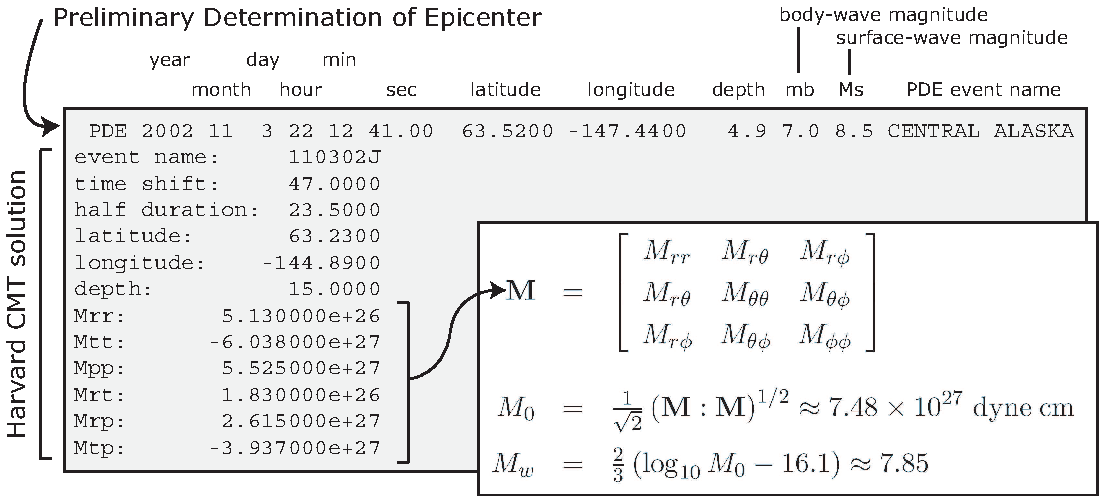
\includegraphics[width=1\textwidth]{figures/Denali_CMT.pdf} }
\par\end{centering}{\small \par}

\caption{\texttt{CMTSOLUTION} file obtained from the Global CMT catalog. The
top line is the initial estimate of the source, which is used as a
starting point for the CMT solution. \textbf{M} is the moment tensor,
$M_{0}${\small{} }is the seismic moment, and $M_{w}$ is the moment
magnitude.}


\label{fig:CMTSOLUTION-file}
\end{figure}
{\small \par}
\end{lyxcode}
The \texttt{CMTSOLUTION} should be edited in the following way:

\begin{itemize}
\item For point-source simulations (see finite sources, page \pageref{To-simulate-a}),
setting the source half-duration parameter \texttt{half duration} equal to zero corresponds to simulating a step source-time
function (Heaviside), i.e., to using a moment-rate function that is a delta function. If
\texttt{half duration} is not set to zero, the code will use a smooth (pseudo) Heaviside source-time function
with a corresponding Gaussian moment-rate function
(i.e., a signal with a shape similar to a `smoothed triangle', as
explained in \citet{KoTr02a} and shown in Fig~\ref{fig:gauss.vs.triangle})
with half-width \texttt{half duration}.

Often, it is preferable to run the solver with \texttt{half duration} set to zero and convolve
the resulting synthetic seismograms in post-processing after the run,
because this way it is easy to use a variety of source-time functions
(see Section \ref{sec:Process-data-and-syn}). \citet{KoTr02a} determined
that the noise generated in the simulation by using a step source
time function may be safely filtered out afterward based upon a convolution
with the desired source-time function and/or low-pass filtering. Use
the postprocessing script \texttt{process\_syn.pl} (see Section \ref{sub:process_syn.pl})
with the \texttt{-h} flag, or the serial code \texttt{convolve\_source\_timefunction.f90}
and the script \texttt{utils/convolve\_source\_timefunction.csh} for
this purpose, or alternatively use signal-processing software packages
such as SAC \urlwithparentheses{http://www.iris.edu/software/sac/}. Type
\begin{verbatim}
make convolve_source_timefunction
\end{verbatim}
to compile the code and then set the parameter \texttt{hdur} in \texttt{utils/convolve\_source\_timefunction.csh}
to the desired half-duration.

\item To use a monochromatic source-time function instead, enable the flag \texttt{USE\_MONOCHROMATIC\_CMT\_SOURCE} in \texttt{Par\_file}. In this case, \texttt{half
duration} will be interpreted as the period of the source-time function. By default, the left side of the source-time function is applied with a Hanning taper at a length of 200.0~s. This can be configured through \texttt{TAPER\_MONOCHROMATIC\_SOURCE} in \texttt{constants.h} file.

\item The zero time of the simulation corresponds to the center of the triangle/Gaussian,
or the centroid time of the earthquake. The start time of the simulation
is $t=-1.5*\texttt{half duration}$ (the 1.5 is to make sure the moment-rate function is very close to zero
when starting the simulation. This avoids spurious high-frequency oscillations).
To convert to absolute time $t_{\mathrm{abs}}$, set

\begin{lyxcode}
$t_{\mathrm{abs}}=t_{\mathrm{pde}}+\texttt{time shift}+t_{\mathrm{synthetic}}$
\end{lyxcode}
where $t_{\mathrm{pde}}$ is the time given in the first line of the
\texttt{CMTSOLUTION}, \texttt{time shift} is the corresponding value
from the original \texttt{CMTSOLUTION} file and $t_{\mathrm{synthetic}}$
is the time in the first column of the output seismogram.

\end{itemize}
%
\begin{figure}
\noindent \begin{centering}
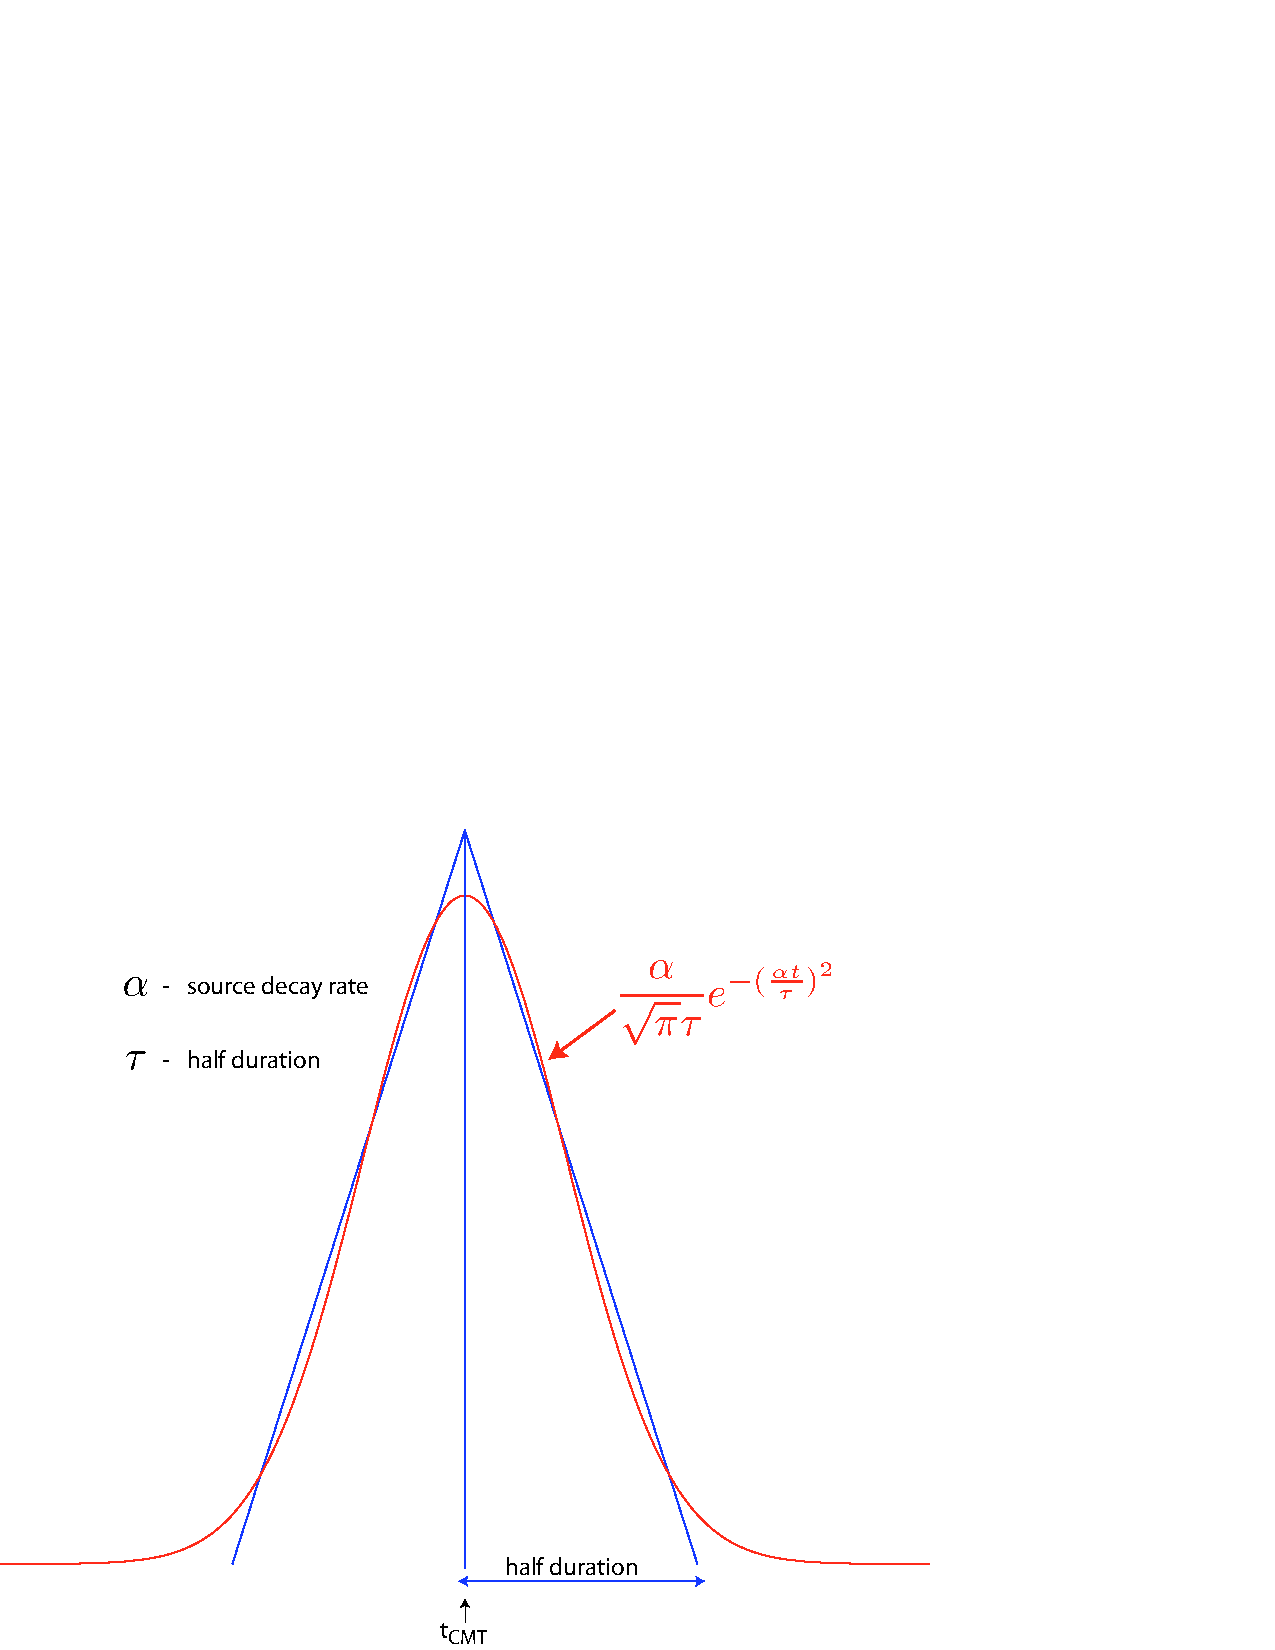
\includegraphics[width=3in]{figures/gauss_vs_triangle_mod.pdf}
\par\end{centering}
\caption{Comparison of the shape of a triangle and the Gaussian function actually used.}
\label{fig:gauss.vs.triangle}
\end{figure}

If you know the earthquake source in strike/dip/rake format rather than in \texttt{CMTSOLUTION} format,
use the C code \texttt{utils/strike\_dip\_rake\_to\_CMTSOLUTION.c} to convert it.
The conversion formulas are given for instance in \cite{AkRi80}.
Note that the \cite{AkRi80} convention is slightly different from the Global/Harvard \texttt{CMTSOLUTION} convention
(the sign of some components is different). The C code outputs both.\newline


Centroid latitude and longitude should be provided in geographical
coordinates. The code converts these coordinates to geocentric coordinates~\citep{DaTr98}.
Of course you may provide your own source representations by designing
your own \texttt{CMTSOLUTION} file. Just make sure that the resulting
file adheres to the Global/Harvard CMT conventions (see Appendix~\ref{cha:Reference-Frame-Convention}).
Note that the first line in the \texttt{CMTSOLUTION} file is the Preliminary Determination of Earthquakes (PDE) solution performed by the USGS NEIC, which is used as a seed for the Global/Harvard CMT inversion. The PDE solution is based upon P waves and often gives the hypocenter of the earthquake, i.e., the rupture initiation point, whereas the CMT solution gives the `centroid location', which is the location with dominant moment release. The PDE solution is not used by our software package but must be present anyway in the first line of the file.\newline


In the current version of the code, the solver can run with a non-zero \texttt{time shift} in the \texttt{CMTSOLUTION} file. Thus one does not need to set \texttt{time shift} to zero as it was the case for previous versions of the code. \texttt{time shift} is only used for writing centroid time in the SAC headers (see Appendix~\ref{cha:SAC-headers}). CMT time is obtained by adding \texttt{time shift} to the PDE time given in the first line in the \texttt{CMTSOLUTION} file. Therefore it is recommended not to modify \texttt{time shift} to have the correct timing information in the SAC headers without any post-processing of seismograms.\newline


\label{To-simulate-a}To simulate a kinematic rupture, i.e., a finite-source
event, represented in terms of $N_{\mathrm{sources}}$ point sources,
provide a \texttt{CMTSOLUTION} file that has $N_{\mathrm{sources}}$
entries, one for each subevent (i.e., concatenate $N_{\mathrm{sources}}$
\texttt{CMTSOLUTION} files to a single \texttt{CMTSOLUTION} file).
At least one entry (not necessarily the first) must have a zero \texttt{time
shift}, and all the other entries must have non-negative \texttt{time
shift}. If none of the entries has a zero \texttt{time shift} in the \texttt{CMTSOLUTION} file, the smallest \texttt{time shift} is subtracted from all sources to initiate the simulation. Each subevent can have its own half duration, latitude, longitude,
depth, and moment tensor (effectively, the local moment-density tensor).\newline


Note that the zero in the synthetics does NOT represent the hypocentral
time or centroid time in general, but the timing of the \textit{center}
of the source triangle with zero \texttt{time shift} (Fig~\ref{fig:source_timing}).
%
\begin{figure}[htp]
\begin{centering}
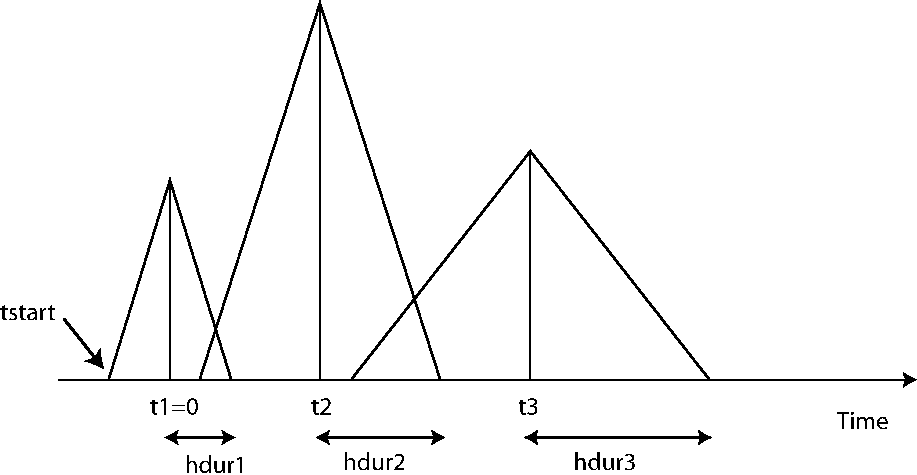
\includegraphics[width=5in]{figures/source_timing.pdf}
\end{centering}
%
\caption{Example of timing for three sources. The center of the first source
triangle is defined to be time zero. Note that this is NOT in general
the hypocentral time, or the start time of the source (marked as tstart).
The parameter \texttt{time shift} in the \texttt{CMTSOLUTION} file
would be t1(=0), t2, t3 in this case, and the parameter \texttt{half duration}
would be hdur1, hdur2, hdur3 for the sources 1, 2, 3 respectively.}
\label{fig:source_timing}
\end{figure}


Although it is convenient to think of each source as a triangle, in
the simulation they are actually Gaussians (as they have better frequency
characteristics). The relationship between the triangle and the Gaussian
used is shown in Fig~\ref{fig:gauss.vs.triangle}. For finite fault
simulations it is usually not advisable to use a zero half duration
and convolve afterwards, since the half duration is generally fixed
by the finite fault model.\newline

\vspace{1cm}

\noindent The \texttt{FORCESOLUTION} file should be edited in the
following way:
\begin{itemize}
\item The first line is only the header for the force solution, which can
be used as the identifier for the force source.
\item \texttt{time shift:} For a single force source, set
this  parameter equal to $0.0$ (The solver will not run otherwise!); the time
shift parameter would simply apply an overall time shift to the synthetics,
something that can be done in the post-processing (see Section \ref{sec:Process-data-and-syn}).
\item \texttt{half duration:} Set the half duration value (s) for step source-time
function. In case that the solver uses a (pseudo) Dirac delta source-time function to represent
a force point source, a very short duration of five time steps is automatically set by default.
For a Ricker source-time function, set the dominant frequency value (Hz).
See the parameter \texttt{source time function:} below for source-time functions.
\item \texttt{latitude:} Set the latitude of the force source.
\item \texttt{longitude:} Set the longitude of the force source.
\item \texttt{depth:} Set the depth of the force source (km).
\item \texttt{source time function:} Set the type of source-time function: 0 = Gaussian function, 1 = Ricker function, 2 = Heaviside (step) function, 3 = monochromatic function, 4 = Gaussian function as defined in \citet{Meschede2011}.
\item \texttt{factor force source:} Set the magnitude of the force source (units in Newton N).
\item \texttt{component dir vect source E:} Set the East component of a direction vector for the force
source. Direction vector is not necessarily a unit vector.
\item \texttt{component dir vect source N:} Set the North component of a direction vector for the force
source.
\item \texttt{component dir vect source Z\_up:} Set the vertical component of a direction vector for the force
source. Sign convention follows the positive upward direction.
\end{itemize}
\noindent Where necessary, set a \texttt{FORCESOLUTION} file in the
same way you configure a \texttt{CMTSOLUTION} file with $N_{\mathrm{sources}}$
entries, one for each subevent (i.e., concatenate $N_{\mathrm{sources}}$
\texttt{FORCESOLUTION} files to a single \texttt{FORCESOLUTION} file).
At least one entry (not necessarily the first) must have a zero \texttt{time
shift}, and all the other entries must have non-negative \texttt{time shift}.
Each subevent can have its own set of parameters \texttt{latitude}, \texttt{longitude}, \texttt{depth},
\texttt{half duration}, etc. \newline


\newpage
The solver can calculate seismograms at any number of stations for
basically the same numerical cost, so the user is encouraged to include
as many stations as conceivably useful in the \texttt{STATIONS} file,
which looks like this:
%
\begin{figure}[htp]
\begin{centering}
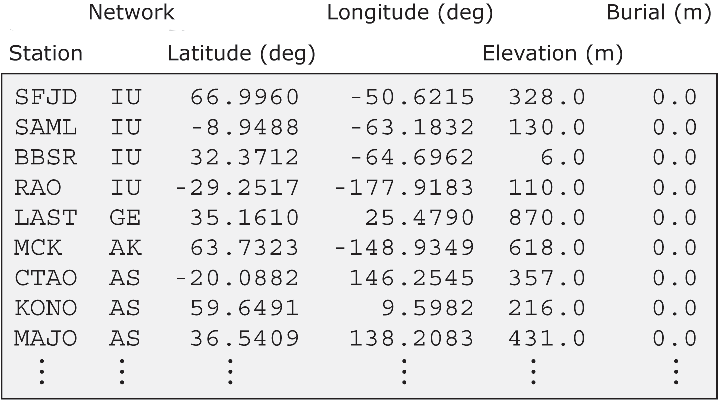
\includegraphics{figures/STATIONS_global_explained.pdf}
\end{centering}
%
\caption{Sample \texttt{STATIONS} file. Station latitude and longitude should
be provided in geographical coordinates. The width of the station
label should be no more than 32 characters (see \texttt{MAX\_LENGTH\_STATION\_NAME}
in the \texttt{constants.h} file), and the network label should be
no more than 8 characters (see \texttt{MAX\_LENGTH\_NETWORK\_NAME}
in the \texttt{constants.h} file).}
\end{figure}

Each line represents one station in the following format:
\begin{verbatim}
Station Network Latitude(degrees) Longitude(degrees) Elevation(m) burial(m)
\end{verbatim}
If you want to put a station on the ocean floor, just set
elevation and burial depth in the STATIONS file to 0.
Equivalently you can also set elevation to a negative value equal
to the ocean depth, and burial depth to 0.\newline


Solver output is provided in the \texttt{OUTPUT\_FILES} directory
in the \texttt{output\_solver.txt} file. Output can be directed to
the screen instead by uncommenting a line in \texttt{constants.h}:
{\small
\begin{verbatim}
! uncomment this to write messages to the screen
! integer, parameter :: IMAIN = ISTANDARD_OUTPUT
\end{verbatim}
}
Note that on very fast machines, writing to the screen may slow down
the code.\newline


While the solver is running, its progress may be tracked by monitoring
the `\texttt{timestamp{*}}' files in the \texttt{OUTPUT\_FILES} directory.
These tiny files look something like this:
{\small
\begin{verbatim}
Time step #           200
Time:    0.6956667      minutes
Elapsed time in seconds =     252.6748970000000
Elapsed time in hh:mm:ss =    0 h 04 m 12 s
Mean elapsed time per time step in seconds =     1.263374485000000
Max norm displacement vector U in solid in all slices (m) =    1.9325
Max non-dimensional potential Ufluid in fluid in all slices = 1.1058885E-22
\end{verbatim}
}
The \texttt{timestamp{*}} files provide the \texttt{Mean elapsed time
per time step in seconds}, which may be used to assess performance
on various machines (assuming you are the only user on a node), as
well as the
\texttt{Max norm displacement vector U in solid in all slices (m)}
and
\texttt{Max non-dimensional potential Ufluid in fluid in all slices}.
If something is wrong with the model, the mesh, or the source, you will see the
code become unstable through exponentionally growing values of the
displacement and/or fluid potential with time, and ultimately the
run will be terminated by the program when either of these values
becomes greater than \texttt{STABILITY\_THRESHOLD} defined in \texttt{constants.h}.
You can control the rate at which the timestamp files are written
based upon the parameter \texttt{NTSTEP\_BETWEEN\_OUTPUT\_INFO} in
the \texttt{Par\_file}.\newline


Having set the \texttt{Par\_file} parameters, and having provided
the \texttt{CMTSOLUTION} and \texttt{STATIONS} files, you are now
ready to launch the solver! This is most easily accomplished based
upon the \texttt{go\_solver} script (see Chapter~\ref{cha:Running-Scheduler}
for information about running the code through a scheduler, e.g.,
LSF). You may need to edit the last command at the end of the script
that invokes the \texttt{mpirun} command. Another option is to use
the \texttt{runall} script, which compiles and runs both mesher and
solver in sequence. This is a safe approach that ensures using the
correct combination of mesher output and solver input.\newline


It is important to realize that the CPU and memory requirements of
the solver are closely tied to choices about attenuation (\texttt{ATTENUATION})
and the nature of the model (i.e., isotropic models are cheaper than
anisotropic models). We encourage you to run a variety of simulations
with various flags turned on or off to develop a sense for what is
involved.\newline


For the same model, one can rerun the solver for different events
by simply changing the \texttt{CMTSOLUTION} file, and/or for different
stations by changing the \texttt{STATIONS} file. There is no need
to rerun the mesher. Of course it is best to include as many stations
as possible, since this does not add significantly to the cost of
the simulation.



\section{Note on the simultaneous simulation of several earthquakes}

\begin{figure}[H]
\begin{centering}
\includegraphics[width=2.2in]{figures/simultaneous_dir_struct.pdf}
\par\end{centering}
%
\caption{
Directory structure when simulating several earthquakes at once.
To improve readability, only directories have been drawn.}
\label{fig:simultaneous_dir_struct}
\end{figure}

Figure~\ref{fig:simultaneous_dir_struct} shows what the directory structure
should looks like when simulating multiple earthquakes at ones.

\begin{itemize}
\item The simulation is launched within the root directory \texttt{EXAMPLE\_ROOT\_DIR}\newline
(usually \texttt{mpirun -np N ./bin/xspecfem3D}).
\item \texttt{DATA} should contain the \texttt{Par\_file} parameter file with
\texttt{NUMBER\_OF\_SIMULTANEOUS\_RUNS} as explained in Chapter~\ref{cha:Running-the-Mesher}.
\item \texttt{DATABASES\_MPI} and {OUTPUT\_FILES} directory may contain the mesher output but they
are not required as they are superseded by the ones in the \texttt{runXXX} directories.
\item \texttt{runXXXX} directories must be created beforehand. There should be be as many as
\texttt{NUMBER\_OF\_SIMULTANEOUS\_RUNS} and the numbering should be contiguous, starting from \texttt{0001}.
They all should have \texttt{DATA},
\texttt{DATABASES\_MPI} and \texttt{OUTPUT\_FILES} directories. Additionally a \texttt{SEM} directory
containing adjoint sources have to be created to perform adjoint simulations.
\item \texttt{runXXXX/DATA} directories must all contain a \texttt{CMTSOLUTION} file,
a \texttt{STATIONS} file along with an eventual \texttt{STATIONS\_ADJOINT} file.
\item If \texttt{BROADCAST\_SAME\_MESH\_AND\_MODEL} is set to \texttt{.true.} in \texttt{DATA/Par\_file},
only \texttt{run0001/OUTPUT\_FILES} and \texttt{run0001/DATABASES\_MPI} directories need to contain the files
outputted by the mesher.
\item If \texttt{BROADCAST\_SAME\_MESH\_AND\_MODEL} is set to \texttt{.false.} in \texttt{DATA/Par\_file},
every \texttt{runXXXX/OUTPUT\_FILES} and \texttt{runXXXX/DATABASES\_MPI} directories need to contain the files
outputted by the mesher. Note that while the meshes might have been created from different models and
parameter sets, they should have been created using the same number of MPI processes.
\end{itemize}





\chapter{Regional Simulations}\label{cha:Regional-Simulations}

%% DK DK got rid of the 2-chunk and 3-chunk options here in the manual (but not in the code) because they are now untested and to my knowledge nobody uses them

The code has the option of running in one-chunk or six-chunk mode.
The one-chunk options may be used for higher resolution regional
simulations. A one-chunk mesh may have lateral dimensions other than
the customary $90^{\circ}$ per chunk, which can further increase
the resolution of the mesh, and thus reduce the shortest period in
the synthetic seismograms (but of course then also reducing the time
step in order for the simulation to remain stable).

A disadvantage of regional simulations is that one needs to use approximate absorbing
boundary conditions on the side and bottom edges of the model (e.g.,
see \citet{KoTr99} for a description of the paraxial boundary conditions
used). Figure~\vref{fig:3D-spectral-element-mesh} and Figure~\vref{fig:Close-up-view-of}
show an example of a one-chunk mesh centered on the Japan subduction
zone, applied in the Japan regional waveform simulation \citep{ChTrHeKa07}.


\section{One-Chunk Simulations}\label{sec:One-Chunk-Simulations}

For a one-chunk regional simulation the following parameters need
to be set in the \texttt{Par\_file}:

\begin{description}
\item [{\texttt{NCHUNKS}}] Must be set to 1.
\item [{\texttt{ANGULAR\_WIDTH\_XI\_IN\_DEGREES}}] Denotes the width of
one side of the chunk ($90^{\circ}$ is a classical value, but you can make it more or less if you want).
\item [{\texttt{ANGULAR\_WIDTH\_ETA\_IN\_DEGREES}}] Denotes the width of
the second side of the chunk ($90^{\circ}$ is a classical value, but you can make it more or less if you want). Note that this
value may be different from \texttt{ANGULAR\_WIDTH\_XI\_IN\_DEGREES}.
\item [{\texttt{CENTER\_LATITUDE\_IN\_DEGREES}}] Defines the latitude of
the center of the chunk (degrees).
\item [{\texttt{CENTER\_LONGITUDE\_IN\_DEGREES}}] Defines the longitude
of the center of the chunk (degrees).
\item [{\texttt{GAMMA\_ROTATION\_AZIMUTH}}] Defines the rotation angle
of the chunk about its center measured counter clockwise from due
North (degrees). The corners of the mesh are output in \texttt{\small OUTPUT\_FILES/values\_from\_mesher.h}.
The output corner progression in \texttt{\small OUTPUT\_FILES/values\_from\_mesher.h}
is bottom left, bottom right, top left, top right. The rotation azimuth
can be changed in the \texttt{Par\_file} and the corners output \texttt{(}\texttt{\small OUTPUT\_FILES/}~\\
\texttt{\small values\_from\_mesher.h}\texttt{)} by using{\small{}
}\texttt{\small xcreate\_header\_file}. It is important to note that
the mesher or the solver does not need to be run to determine the
limits of a 1-chunk simulation.
\item [{\texttt{NEX\_XI}}] The number of spectral elements along the $\xi$ side
of the chunk. This number \textit{must} be 8~$\times$~a multiple
of $\nprocxi$ defined below. For a $90^{\circ}$ chunk, we do not
recommend using $\nexxi$ less than~64 because the curvature of the
Earth cannot be honored if one uses too few elements, which results
in inaccurate and unstable simulations.
\item [{\texttt{NEX\_ETA}}] The number of spectral elements along the $\eta$
side of the chunk. This number \textit{must} be 8~$\times$~a multiple
of $\nproceta$ defined below. Note that in order to get elements
that are close to square on the Earth's surface, the following ratios
should be similar:
\begin{verbatim}
ANGULAR_WIDTH_XI_IN_DEGREES / NEX_XI
ANGULAR_WIDTH_ETA_IN_DEGREES / NEX_ETA
\end{verbatim}
Because of the geometry of the cubed sphere, the option of having
different values for $\nexxi$ and $\nexeta$ is available only for
regional simulations when $\nchunks=1$ (1/6th of the sphere).

\item [{\texttt{NPROC\_XI}}] The number of processors or mesh slices along the
$\xi$ side of the chunk. To accommodate the mesh doubling layers,
we must have $\nexxi=8\times c\times\nprocxi$, where $c\ge1$ is
a positive integer. See Table~\ref{table:nex} for various suitable
choices.
\item [{\texttt{NPROC\_ETA}}] The number of processors or slices along the $\eta$
side of the chunk; we must have $\nexeta=8\times c\times\nproceta$,
where $c\ge1$ is a positive integer. $\nprocxi$ and $\nproceta$
must be equal when $\nchunks=6$.
\end{description}
%
\begin{figure}[H]
\begin{centering}
\includegraphics[scale=0.65]{figures/fig5a.jpg}
\par\end{centering}

\caption{S-wave velocity anomalies
from the global tomographic model s20rts \citep{RiVa00} are superimposed
on the mesh. For parallel computing purposes, the one-chunk SEM simulation
is subdivided in terms of 64 slices. The center of the chunk is at
(38.5$^{\circ}$ N, 137.5$^{\circ}$ E), and the lateral dimensions
are 30$^{\circ}$ $\times$ 30$^{\circ}$. Two doubling layers are
indicated at a depth of 25~km (PREM Moho depth) and a depth of about
1650~km. Shows full view of 25 neighboring slices; see Figure~\ref{fig:Close-up-view-of}
for close-up of upper mantle mesh.}
\label{fig:3D-spectral-element-mesh}
\end{figure}
%
\begin{figure}[H]
\begin{centering}
\includegraphics[scale=0.65]{figures/fig5b.jpg}
\par\end{centering}

\caption{Close-up view of the upper mantle
mesh shown in Figure~\ref{fig:3D-spectral-element-mesh}. Note that
the element size in the crust (top layer) is 13~km $\times$ 13~km,
and that the size of the spectral elements is doubled in the upper
mantle. The velocity variation is captured by NGLL = 5 grid points
in each direction of the elements \citep{KoTr02a,KoTr02b}.}
\label{fig:Close-up-view-of}
\end{figure}


\begin{description}
\item [{\texttt{ABSORBING\_CONDITIONS}}] Set to \texttt{.true.}{\small{}
}for regional simulations. For instance, see \citet{KoTr99} for a
description of the paraxial boundary conditions used. Note that these
conditions are never perfect, and in particular surface waves may
partially reflect off the artificial boundaries. Note also that certain
arrivals, e.g., PKIKPPKIKP, will be missing from the synthetics.
\end{description}
When the width of the chunk is different from $90^{\circ}$ (or the
number of elements is greater than 1248), the radial distribution
of elements needs to be adjusted as well to maintain spectral elements
that are as cube-like as possible. The code attempts to do this, but
be sure to view the mesh with your favorite graphics package to make
sure that the element are well behaved.
Remember: a high-quality mesh is paramount for accurate simulations.
In addition to a reorganization of the radial distribution of elements,
the time stepping and period range in which the attenuation is applied
is automatically determined. The minimum and maximum periods for attenuation
are:

\[
\omega_{max}=\omega_{min}\times10^{W_{3}}\]


\noindent where $W_{3}$ is the optimal width in frequency for 3 Standard
Linear Solids, about 1.75. See \texttt{\small read\_compute\_parameters.f90}
for more details.

The time stepping is determined in a similar fashion as Equation (48)
in \citet{KoTr02a}:

\begin{lyxcode}
dt~=~$S_{c}$~Element~Width~in~km~($r=$ICB)~/~Velocity~($r=$ICB)
\end{lyxcode}
where $S_{c}$ is the stability condition (about 0.4). We use the
radius at the inner core boundary because this is where the maximum
velocity/element width occurs. Again, see \texttt{\small read\_compute\_parameters}\texttt{.f90}
for all the details.

The approximate shortest period at which a regional simulation is
accurate may be determined based upon the relation
\begin{equation}
\mbox{shortest period (s)}\simeq(256/\nexxi)\times(\texttt{ANGULAR\_WIDTH\_XI\_IN\_DEGREES}/90)\times17.\label{eq:shortest_period_regional}\end{equation}



% \section{Two-Chunk Simulations}
%
% For a two-chunk regional simulation the following parameters need
% to be set in the \texttt{Par\_file}:
%
% \begin{description}
% \item [{$\nchunks$}] Must be set to 2
% \item [{\texttt{ANGULAR\_WIDTH\_XI\_IN\_DEGREES}}] Denotes the width of
% one side of the chunk, and it has to be 90 degrees.
% \item [{\texttt{ANGULAR\_WIDTH\_ETA\_IN\_DEGREES}}] Denotes the width of
% the second side of the chunk, and it also has to be 90 degrees.
% \end{description}
% \texttt{NEX\_XI} and \texttt{NEX\_ETA} follow the same description
% in Section \ref{sec:One-Chunk-Simulations}, however, they need to
% be the same in this case. All other parameters are similar to the
% one-chunk simulations, refer to Section \ref{sec:One-Chunk-Simulations}
% for details.
%
% %
% \begin{figure}[H]
% \noindent \begin{centering}
% 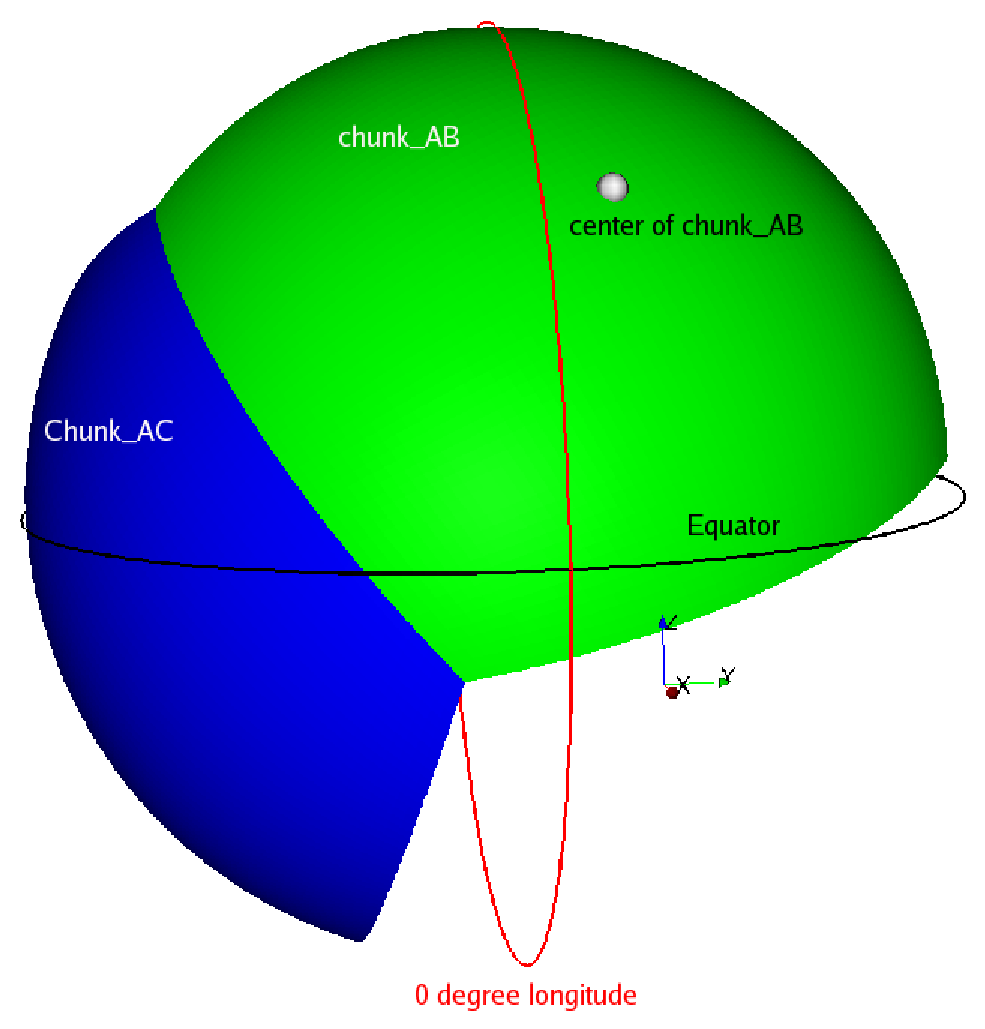
\includegraphics[width=0.6\textwidth]{figures/2-chunk-surface}
% \par\end{centering}
%
% \caption{Geometry of a 2-chunk simulation, where the first chunk (\texttt{CHUNK\_AB})
% centers at $40^{\circ}$ latitude, $10^{\circ}$ longitude, and has
% been rotated by $20^{\circ}$ counter clockwise, and the second chunk
% (\texttt{CHUNK\_AC}) connects to the first chunk through one face.}
%
% \end{figure}






\chapter{Adjoint Simulations}\label{cha:Adjoint-Simulations}

Adjoint simulations are generally performed for two distinct applications.
First, they can be used for earthquake source inversions, especially
earthquakes with large ruptures such as the Sumatra-Andaman event
\citep{LayKanamoriAmmon2005,AmmonJiThio2005,ParkSongTromp2005}. Second,
they can be used to generate finite-frequency sensitivity kernels
that are a critical part of tomographic inversions based upon 3D reference
models \citep{TrTaLi05,LiTr06,TrKoLi08,LiTr08}. In either case, source
parameter or velocity structure updates are sought to minimize a specific
misfit function (e.g., waveform or traveltime differences), and the
adjoint simulation provides a means of computing the gradient of the
misfit function and further reducing it in successive iterations.
Applications and procedures pertaining to source studies and finite-frequency
kernels are discussed in Sections~\ref{sec:Adjoint-simulation-sources}
and \ref{sec:Adjoint-simulation-finite}, respectively. The two related
parameters in the \texttt{Par\_file} are \texttt{SIMULATION\_TYPE}
(1, 2 or 3) and \texttt{SAVE\_FORWARD} (boolean).


\section{Adjoint Simulations for Sources Only (not for the Model)}\label{sec:Adjoint-simulation-sources}

In the case where a specific misfit function is minimized to invert
for the earthquake source parameters, the gradient of the misfit function
with respect to these source parameters can be computed by placing
time-reversed seismograms at the receivers and using them as sources
in an adjoint simulation, and then the value of the gradient is obtained
from the adjoint seismograms recorded at the original earthquake location.

\begin{enumerate}
\item \textbf{Prepare the adjoint sources} \label{enu:Prepare-the-adjoint}

\begin{enumerate}
\item First, run a regular forward simlation (\texttt{SIMULATION\_TYPE =
1} and \texttt{SAVE\_FORWARD = .false.}). You can automatically set
these two variables using the \texttt{\small utils/change\_simulation\_type.pl}
script:
\begin{verbatim}
utils/change_simulation_type.pl -f
\end{verbatim}
and then collect the recorded seismograms at all the stations given
in \texttt{DATA/STATIONS}.

\item Then select the stations for which you want to compute the time-reversed
adjoint sources and run the adjoint simulation, and compile them into
the \texttt{DATA/STATIONS\_ADJOINT} file, which has the same format
as the regular \texttt{DATA/STATIONS} file.

\begin{itemize}
\item Depending on what type of misfit function is used for the source inversion,
adjoint sources need to be computed from the original recorded seismograms
for the selected stations and saved in the \texttt{SEM/} directory
with the format \texttt{NT.STA.?X?.adj}, where \texttt{STA}, \texttt{NT}
are the station name and network code given in the \texttt{DATA/STATIONS\_ADJOINT}
file, and \texttt{?X?}  represents the channel name of a particular
adjoint seismogram where the first letter corresponds to the band code governed by the resolution of simulations, for example, generally \texttt{MX?} for the current resolution of global simulations (see Appendix~\ref{cha:channel-codes} for details). The last letter of channel names is the component name \texttt{E/N/Z}.
\item The adjoint seismograms are in the same format as the original seismogram
(\texttt{NT.STA.?X?.sem?}), with the same start time, time interval
and record length.
\end{itemize}
\item Notice that even if you choose to time reverse only one component
from one specific station, you still need to supply all three components
because the code is expecting them (you can set the other two components
to be zero).
\item Also note that since time-reversal is done in the code itself, no
explicit time-reversing is needed for the preparation of the adjoint
sources, i.e., the adjoint sources are in the same forward time sense
as the original recorded seismograms.
\end{enumerate}

\item \textbf{Set the related parameters and run the adjoint simulation}\\
In the \texttt{DATA/Par\_file}, set the two related parameters to
be \texttt{SIMULATION\_TYPE = 2} and \texttt{SAVE\_FORWARD = .false.}.
More conveniently, use the scripts \texttt{utils/change\_simulation\_type.pl}
to modify the \texttt{Par\_file} automatically (\texttt{change\_simulation\_type.pl
-a}). Then run the solver to launch the adjoint simulation.

\item \textbf{Collect the seismograms at the original source location}\\
After the adjoint simulation has completed successfully, get the seismograms
from directory \texttt{OUTPUT\_FILES}.
%
\begin{itemize}
\item These adjoint seismograms are recorded at the locations of the original
earthquake sources given by the \texttt{DATA/CMTSOLUTION} file, and
have names of the form \texttt{NT.S?????.S??.sem} for the six-component
strain tensor (\texttt{SNN,SEE,SZZ,SNE,SNZ,SEZ}) at these locations,
and \texttt{NT.S?????.?X?.sem} for the three-component displacements
(i.e., \texttt{MXN,MXE,MXZ}) recorded at these locations.
\item \texttt{S?????} denotes the source number; for example, if the original
\texttt{CMTSOLUTION} provides only a point source, then the seismograms
collected will start with \texttt{S00001}.
\item These adjoint seismograms provide critical information for the computation
of the gradient of the misfit function.
\end{itemize}
\end{enumerate}



\section{Adjoint Simulations for Finite-Frequency Kernels (Kernel Simulation)}\label{sec:Adjoint-simulation-finite}

Finite-frequency sensitivity kernels are computed in two successive
simulations (please refer to \citet{LiTr06} and \citet{TrKoLi08} for details).

\begin{enumerate}
\item \textbf{Run a forward simulation with the state variables saved at
the end of the simulation}


Prepare the \texttt{\small CMTSOLUTION} and \texttt{\small STATIONS}
files, set the parameters \texttt{\small SIMULATION\_TYPE}{\small{}
}\texttt{\small =}{\small{} }\texttt{\small 1} and \texttt{\small SAVE\_FORWARD
=}{\small{} }\texttt{\small .true.} in the \texttt{Par\_file} (\texttt{change\_simulation\_type
-F}), and run the solver.

\begin{itemize}
\item Notice that attenuation is not fully implemented yet for the computation
of finite-frequency kernels; if \texttt{ATTENUATION = .true.} is set
in the \texttt{Par\_file}, only effects on phase shift are accounted for
but not on amplitude of the signals. However, we suggest you use the same
setting for \texttt{ATTENUATION} as for your forward simulations.
\item We also suggest you modify the half duration of the \texttt{CMTSOLUTION}
to be similar to the accuracy of the simulation (see Equation \ref{eq:shortest_period}
or \ref{eq:shortest_period_regional}) to avoid too much high-frequency
noise in the forward wavefield, although theoretically the high-frequency
noise should be eliminated when convolved with an adjoint wavefield
with the proper frequency content.
\item This forward simulation differs from the regular simulations (\texttt{\small SIMULATION\_TYPE}{\small{}
}\texttt{\small =}{\small{} }\texttt{\small 1} and \texttt{\small SAVE\_FORWARD}{\small{}
}\texttt{\small =}{\small{} }\texttt{\small .false.}) described in
the previous chapters in that the state variables for the last time
step of the simulation, including wavefields of the displacement,
velocity, acceleration, etc., are saved to the \texttt{LOCAL\_PATH}
to be used for the subsequent simulation.
\item For regional simulations, the files recording the absorbing boundary
contribution are also written to the \texttt{LOCAL\_PATH} when \texttt{SAVE\_FORWARD
= .true.}.
\end{itemize}


\item \textbf{Prepare the adjoint sources}


The adjoint sources need to be prepared the same way as described
in Section~\ref{sec:Adjoint-simulation-sources}, item~\ref{enu:Prepare-the-adjoint}.

\begin{itemize}
\item In the case of traveltime finite-frequency kernel for one source-receiver
pair, i.e., point source from the \texttt{CMTSOLUTION}, and one station
in the \texttt{STATIONS\_ADJOINT} list, we supply a sample program
in \texttt{utils/adjoint\_sources/traveltime} to cut a certain portion of the original
displacement seismograms and convert them into the proper adjoint
source to compute the finite-frequency kernel.
\begin{lyxcode}
xcreate\_adjsrc\_traveltime~t1~t2~ifile{[}0-5]~E/N/Z-ascii-files~{[}baz]
\end{lyxcode}
where \texttt{t1} and \texttt{t2} are the start and end time of the
portion you are interested in, \texttt{ifile} denotes the component
of the seismograms to be used (0 for all three components, 1 for east,
2 for north, and 3 for vertical, 4 for transverse, and 5 for radial
component), \texttt{E/N/Z-ascii-files} indicate the three-component
displacement seismograms in the right order, and \texttt{baz} is the
back-azimuth of the station from the event location. Note that \texttt{baz}
is only supplied when \texttt{ifile} = 4 or 5.

\item Similarly, a sample program to compute adjoint sources for amplitude finite-frequency kernels may be found in \texttt{utils/adjoint\_sources/amplitude} and used in the same way as described
for traveltime measurements
\begin{lyxcode}
xcreate\_adjsrc\_amplitude~t1~t2~ifile{[}0-5]~E/N/Z-ascii-files~{[}baz].
\end{lyxcode}
\end{itemize}

For adjoint runs (SIMULATION\_TYPE = 3), the adjoint sources need to be put in the "SEM" sub-directory in the root directory of the code.

If your adjoint source have names of the following form for instance:

NET.STA00.MXZ.sem.ascii.adj
NET.STA00.MXZ.sem.ascii.adj

you will need to rename them to:

NET.STA00.MXZ.adj
NET.STA00.MXZ.adj

i.e. suppress ".sem.ascii".

You will also need to create a file called STATIONS\_ADJOINT in the "DATA" directory in the root directory of the code. That file can be identical to the DATA/STATIONS file if you had a single station in STATIONS.


\item \textbf{Run the kernel simulation}


With the successful forward simulation and the adjoint source ready
in \texttt{SEM/}, set \texttt{SIMULATION\_TYPE = 3} and \texttt{SAVE\_FORWARD
= .false.} in the \texttt{Par\_file(change\_simulation\_type.pl -b)},
and rerun the solver.

\begin{itemize}
\item The adjoint simulation is launched together with the back reconstruction
of the original forward wavefield from the state variables saved from
the previous forward simulation, and the finite-frequency kernels
are computed by the interaction of the reconstructed forward wavefield
and the adjoint wavefield.
\item The back-reconstructed seismograms at the original station locations
are saved to the \texttt{OUTPUT\_FILES} directory at the end of the
kernel simulations.
\item These back-constructed seismograms can be compared with the time-reversed
original seismograms to assess the accuracy of the backward reconstruction,
and they should match very well (in the time-reversed sense).
\item The files containing the density, P-wave speed and S-wave speed kernels
are saved in the \texttt{LOCAL\_PATH} with the names of \texttt{proc??????\_reg\_?\_rho(alpha,beta)\_kernel.bin},
where \texttt{proc??????} represents the processor number, and \texttt{reg\_?}
denotes the region these kernels are for, including mantle (\texttt{reg\_1}),
outer core (\texttt{reg\_2}), and inner core (\texttt{reg\_3}). The
output kernels are in the unit of $s/km^{3}$.
\item Note that if you set the flag \texttt{APPROXIMATE\_HESS\_KL = .true.} in
the \texttt{constants.h} file and recompile the solver, the adjoint simulation
also saves files \texttt{proc??????\_reg\_1\_hess\_kernel.bin} which can
be used as preconditioners in the crust-mantle region for iterative inverse
optimization schemes.
\end{itemize}
\item \textbf{Run the boundary kernel simulation}


\noindent If you set the \texttt{SAVE\_BOUNDARY\_MESH = .true.} in
the \texttt{constants.h} file before the simulations, i.e., at the
beginning of step 1, you will get not only the volumetric kernels
as described in step 3, but also boundary kernels for the Earth's
internal discontinuities, such as Moho, 410-km discontinuity, 670-km
discontinuity, CMB and ICB. These kernel files are also saved in the
local scratch directory defined by \texttt{LOCAL\_PATH }and have names
such as \texttt{proc??????\_reg\_1(2)\_Moho(d400,d670,CMB,ICB)\_kernel.bin}.
For a theoretical derivation of the boundary kernels, refer to \citet{TrTaLi05},
and for the visualization of the boundary kernels, refer to Section
\ref{sec:Finite-Frequency-Kernels}.

\item \textbf{Run the anisotropic kernel simulation}


Instead of the kernels for the isotropic wave speeds, you can also
compute the kernels for the 21 independent components $C_{IJ},\, I,J=1,...,6$
(using Voigt's notation) of the elastic tensor in the (spherical)
geographical coordinate system. This is done by setting \texttt{ANISOTROPIC\_KL}
\texttt{=} \texttt{.true.} in \texttt{constants.h} before step 3.
The definition of the parameters $C_{IJ}$ in terms of the corresponding
components $c_{ijkl},ijkl,i,j,k,l=1,2,3$ of the elastic tensor in
spherical coordinates follows \citet{ChTr07}. The computation of
the anisotropic kernels is only implemented in the crust and mantle
regions. The 21 anisotropic kernels are saved in the \texttt{LOCAL\_PATH}
in one file with the name of \texttt{proc??????\_reg1\_cijkl\_kernel.bin}
(with \texttt{proc??????} the processor number). The output kernels
correspond to perturbation $\delta C_{IJ}$ of the elastic parameters
and their unit is in $s/GPa/km^{3}$. For consistency, the output
density kernels with this option turned on are for a perturbation
$\delta\rho$ (and not $\frac{\delta\rho}{\rho}$) and their unit
is in s / (kg/m$^{3}$) / km$^{3}$. These `primary' anisotropic kernels
can then be combined to obtain the kernels related to other descriptions
of anisotropy. This can be done, for example, when combining the kernel
files from slices into one mesh file (see Section~\ref{sec:Finite-Frequency-Kernels}).

\end{enumerate}
In general, the first three steps need to be run sequentially to ensure
proper access to the necessary files at different stages. If the simulations
are run through some cluster scheduling system (e.g., LSF), and the
forward simulation and the subsequent kernel simulations cannot be
assigned to the same set of computer nodes, the kernel simulation
will not be able to access the database files saved by the forward
simulation. Solutions for this problem are provided in Chapter~\ref{cha:Running-Scheduler}.
Visualization of the finite-frequency kernels is discussed in Section~\ref{sec:Finite-Frequency-Kernels}.





\chapter{Doing tomography, i.e., updating the model based on the sensitivity kernels obtained}


The process is described in the same chapter of the manual of SPECFEM3D. Please refer to it.





\chapter{Noise Cross-correlation Simulations}


The new version of SPECFEM3D\_GLOBE includes functionality for seismic noise tomography.
Users are recommended to familiarize themselves first with the procedures for running regular earthquake
simulations (Chapters \ref{cha:Running-the-Mesher}--\ref{cha:Regional-Simulations}) and
adjoint simulations (Chapter \ref{cha:Adjoint-Simulations}).
Also, make sure you read the paper `Noise cross-correlation sensitivity kernels' \citep{trompetal2010}
in order to understand noise simulations from a theoretical perspective.

\section{New Requirements on `Old' Input Parameter Files}

As usual, the three main input files are crucial: \texttt{DATA/Par\_file}, \texttt{DATA/CMTSOLUTION} and
\texttt{DATA/STATIONS}.\newline


\texttt{DATA/CMTSOLUTION} is required for all simulations. However, it may seem unexpected to have it listed here, since the
noise simulations should have nothing to do with the earthquake -- hence the \texttt{DATA/CMTSOLUTION}.
For noise simulations, it is critical to have no earthquakes. In other words, the moment tensor
specified in \texttt{DATA/CMTSOLUTION} must be set to ZERO! \newline


\texttt{DATA/STATIONS} remains the same as in previous earthquake simulations,
except that the order of stations listed in \texttt{DATA/STATIONS} is now important.
The order will be used later to identify the `main' receiver,
i.e., the one that simultaneously cross correlates with the others.
Please be noted that the actual station file used in the simulation is \texttt{OUTPUT\_FILES/STATIONS\_FILTERED},
which is generated when you run your simulations. (e.g., in regional simulations we may have included stations out of the
region of our interests in \texttt{DATA/STATIONS}, so we have to get rid of them.)\newline


\texttt{DATA/Par\_file} also requires careful attention.
New to this version of SPECFEM3D\_GLOBE, a parameter called \texttt{NOISE\_TOMOGRAPHY} has been added that specifies the type of simulation to be run.
\texttt{NOISE\_TOMOGRAPHY} is an integer with possible values 0, 1, 2 and 3.
For example, when \texttt{NOISE\_TOMOGRAPHY} equals 0, a regular earthquake simulation will be run.
When \texttt{NOISE\_TOMOGRAPHY} is equal to 1/2/3, you are about to run
step 1/2/3 of the noise simulations respectively.
Should you be confused by the three steps, refer to \citet{trompetal2010} for details.\newline


Another change to \texttt{DATA/Par\_file} involves the parameter \texttt{RECORD\_LENGTH\_IN\_MINUTES}.
While for regular earthquake simulations this parameter specifies the length of synthetic seismograms generated,
for noise simulations it specifies the length of the seismograms used to compute cross correlations.
The actual cross correlations are thus twice this length.
The code automatically makes modification accordingly, if \texttt{NOISE\_TOMOGRAPHY} is not zero.\newline


There are other parameters in \texttt{DATA/Par\_file} which should be given specific values.
For instance, \texttt{NUMBER\_OF\_RUNS} and \texttt{NUMBER\_OF\_THIS\_RUN} must be 1;
\texttt{ROTATE\_SEISMOGRAMS\_RT}, \texttt{SAVE\_ALL\_SEISMOGRAMS\_IN\_ONE\_FILES},
\texttt{USE\_BINARY\_FOR\_LARGE\_FILE} and \texttt{MOVIE\_COARSE} should be \texttt{.false.}.
Moreover, since the first two steps for calculating noise cross-correlation kernels correspond to
forward simulations, \texttt{SIMULATION\_TYPE} must be 1 when \texttt{NOISE\_TOMOGRAPHY} equals 1 or 2.
Also, we have to reconstruct the ensemble forward wavefields in adjoint simulations,
therefore we need to set \texttt{SAVE\_FORWARD} to \texttt{.true.} for the second step,
i.e., when \texttt{NOISE\_TOMOGRAPHY} equals 2.
The third step is for kernel constructions. Hence \texttt{SIMULATION\_TYPE} should be 3, whereas
\texttt{SAVE\_FORWARD} must be \texttt{.false.}.\newline


\section{Noise Simulations: Step by Step}

Proper parameters in those `old' input files are not enough for noise simulations to run.
We have a lot more `new' input parameter files to specify:
for example, the ensemble-averaged noise spectrum, the noise distribution etc.
However, since there are a few `new' files, it is better to introduce them sequentially.
Read through this section even if you don't understand some parts temporarily,
since some examples you can go through are provided in this package.

\subsection{Pre-simulation}

\begin{itemize}

\item
As usual, we first configure the software package using:
\begin{verbatim}
./configure FC=ifort MPIFC=mpif90
\end{verbatim}

\item
Next, we need to compile the source code using:
\begin{verbatim}
make xmeshfem3D
make xspecfem3D
\end{verbatim}

Before compilation, the \texttt{DATA/Par\_file} must be specified correctly, e.g.,
\texttt{NOISE\_TOMOGRAPHY} shouldn't be zero; \texttt{RECORD\_LENGTH\_IN\_MINUTES},
\texttt{NEX\_XI} and \texttt{NEX\_ETA} must be what you want in your real simulations.
Otherwise you may get wrong informations which will cause problems later.
(it is good to always re-complie the code before you run simulations)\newline

\item
After compiling, you will find two important numbers besides the needed executables:
\begin{verbatim}
number of time steps = 31599
time_stepping of the solver will be: 0.19000
\end{verbatim}

The first number will be denoted as \texttt{NSTEP} from now on, and the second one as \texttt{dt}.
The two numbers are essential to calculate the ensemble-averaged noise spectrum from either Peterson's noise
model or just a simple flat power spectrum (corresponding to 1-bit preprocessing).
Should you miss the two numbers, you can run
\texttt{./xcreate\_header\_file} to bring them up again (with correct \texttt{DATA/Par\_file}!).
FYI, \texttt{NSTEP} is determined by \texttt{RECORD\_LENGTH\_IN\_MINUTES} in \texttt{DATA/Par\_file},
which is automatically doubled in noise simulations; whereas \texttt{dt} is derived from
\texttt{NEX\_XI} and \texttt{NEX\_ETA}, or in other words your element sizes.


\item
A Matlab script is provided to generate the ensemble-averaged noise spectrum.
\begin{verbatim}
EXAMPLES/noise_examples/NOISE_TOMOGRAPHY.m  (main program)
EXAMPLES/noise_examples/PetersonNoiseModel.m
\end{verbatim}

In Matlab, simply run:
\begin{verbatim}
NOISE_TOMOGRAPHY(NSTEP, dt, Tmin, Tmax, NOISE_MODEL)
\end{verbatim}

\texttt{NSTEP} and \texttt{dt} have been given when compiling the specfem3D source code;
\texttt{Tmin} and \texttt{Tmax} correspond to the period range you are interested in;
\texttt{NOISE\_MODEL} denotes the noise model you will be using.
Details can be found in the Matlab script.

After running the Matlab script, you will be given the following information (plus a figure in Matlab):
\begin{verbatim}
*************************************************************
the source time function has been saved in:
/data2/yangl/3D_NOISE/S_squared         (note this path must be different)
S_squared should be put into directory:
./NOISE_TOMOGRAPHY/ in the SPECFEM3D_GLOBE package
\end{verbatim}

In other words, the Matlab script creates a file called \texttt{S\_squared},
which is the first `new' input file we encounter for noise simulations.

One may choose a flat noise spectrum rather than Peterson's noise model.
This can be done easily by modifying the Matlab script a little bit.

\item
Create a new directory in the SPECFEM3D\_GLOBE package, name it as \texttt{NOISE\_TOMOGRAPHY}.
In fact, this new directory should have been created already when checking out the package.
We will add/replace some information needed in this folder.

\item
Put the Matlab-generated-file \texttt{S\_squared} in \texttt{NOISE\_TOMOGRAPHY}.

That's to say, you will have a file \texttt{NOISE\_TOMOGRAPHY/S\_squared} in the SPECFEM3D\_GLOBE package.

\item
Create a file called \texttt{NOISE\_TOMOGRAPHY/irec\_main\_noise}. Note that this file should be put
in directory \texttt{NOISE\_TOMOGRAPHY} as well. This file contains only one integer, which is the ID
of the `main' receiver. For example, if in this file shows 5, it means that the fifth receiver
listed in \texttt{DATA/STATIONS} becomes the `main'. That's why we mentioned previously that
the order of receivers in \texttt{DATA/STATIONS} is important.

Note that in regional (1- or 2-chunk) simulations, the \texttt{DATA/STATIONS}
may contain receivers not within the selected chunk(s).
Therefore, the integer in \texttt{NOISE\_TOMOGRAPHY/irec\_main\_noise}
is actually the ID in \texttt{DATA/STATIONS\_FILTERED} (which is generated by \texttt{xspecfem3D}).

\item
Create a file called \texttt{NOISE\_TOMOGRAPHY/nu\_main}. This file holds three numbers,
forming a (unit) vector. It describes which component we are cross-correlating at the `main'
receiver, i.e., ${\hat{\bf \nu}}^{\alpha}$ in \citet{trompetal2010}. The three numbers correspond to
N/E/Z components respectively.

\item
Describe the noise direction and distributions in \texttt{src/specfem3d/noise\_tomography.f90}.
Search for a subroutine called \texttt{noise\_distribution\_direction}
in \texttt{noise\_tomography.f90}. It is actually located at the very beginning
of \texttt{noise\_tomography.f90}. The default assumes vertical noises and a uniform distribution
across the whole physical domain. It should be quite self-explanatory for modifications.
Should you modify this part, you have to re-compile the source code. (again, that's why we recommend
that you always re-compile the code before you run simulations)

\end{itemize}

\subsection{Simulations}

As discussed in \citet{trompetal2010}, it takes three simulations to obtain one contribution
of the ensemble sensitivity kernels:

\begin{itemize}
\item
Step 1: simulation for generating wavefield
\begin{verbatim}
SIMULATION_TYPE = 1
NOISE_TOMOGRAPHY = 1
SAVE_FORWARD  not used, can be either .true. or .false.
\end{verbatim}

\item
Step 2: simulation for ensemble forward wavefield
\begin{verbatim}
SIMULATION_TYPE = 1
NOISE_TOMOGRAPHY = 2
SAVE_FORWARD = .true.
\end{verbatim}

\item
Step 3: simulation for ensemble adjoint wavefield and sensitivity kernels
\begin{verbatim}
SIMULATION_TYPE = 3
NOISE_TOMOGRAPHY = 3
SAVE_FORWARD = .false.
\end{verbatim}

Note Step 3 is an adjoint simulation, please refer to previous chapters on how to prepare adjoint sources
and other necessary files, as well as how adjoint simulations work.

\end{itemize}

It's better to run the three steps continuously within the same job, otherwise you have to collect the saved surface movies
from the old nodes to the new nodes.\newline

\subsection{Post-simulation}

After those simulations, you have all stuff you need, either in the \texttt{OUTPUT\_FILES} or
in the directory specified by \texttt{LOCAL\_PATH} in \texttt{DATA/Par\_file} (most probably on local nodes).
Collect whatever you want from the local nodes to your workstation, and then visualize them.
This process is the same as what you may have done for regular earthquake simulations.
Refer Chapter~\ref{cha:graphics} if you have problems.\newline


Simply speaking, two outputs are the most interesting: the simulated ensemble cross correlations and
one contribution of the ensemble sensitivity kernels.\newline


The simulated ensemble cross correlations are obtained after the second simulation (Step 2).
Seismograms in \texttt{OUTPUT\_FILES} are actually the simulated ensemble cross correlations.
Collect them immediately after Step 2, or the Step 3 will overwrite them.
Note that we have a `main' receiver specified by \texttt{NOISE\_TOMOGRAPHY/irec\_main\_noise},
the seismogram at one station corresponds to the cross correlation between that station and the `main'.
Since the seismograms have three components, we may obtain cross correlations
for different components as well, not necessarily the cross correlations between vertical components.\newline


One contribution of the ensemble cross-correlation sensitivity kernels are obtained after Step 3,
stored in the \texttt{LOCAL\_PATH} on local nodes.
The ensemble kernel files are named the same as regular earthquake kernels.\newline


You need to run another three simulations to get the other contribution of the ensemble kernels,
using different forward and adjoint sources given in \citet{trompetal2010}.

\section{Examples}

In order to illustrate noise simulations in an easy way, three examples are provided in
\texttt{EXAMPLES/noise\_examples/}.
Note however that they are created for a specific cluster (SESAME@PRINCETON).
You have to modify them to fit your own cluster.

The three examples can be executed using (in directory \texttt{EXAMPLES/noise\_examples/}):
\begin{verbatim}
./run_this_example.sh regional
./run_this_example.sh global_short
./run_this_example.sh global_long
\end{verbatim}

Each corresponds to one example, but they are pretty similar.

Although the job submission only works on SESAME@PRINCETON, the procedure itself is universal.
You may review the whole process described in the last section by following commands in those examples.

Finally, note again that those examples show only one contribution of the ensemble kernels!






\chapter{Gravity integral calculations for the gravity field of the Earth}


SPECFEM can now compute the gravity field as well as its derivatives (i.e., gravity gradiometry)
generated by any given 3D Earth model at the height
of an observation satellite, for instance GOCE\newline
(see e.g. en.wikipedia.org/wiki/Gravity\_Field\_and\_Steady-State\_Ocean\_Circulation\_Explorer).\newline
That feature is still experimental but should work just fine.\newline


\noindent
To see how it is implemented and to use it, type this in the root directory of the code:
\begin{verbatim}
grep -i GRAVITY_INTEGRALS src/*/*
\end{verbatim}
All main gravity field computations can be found in file \texttt{src/meshfem3d/gravity\_integrals.F90}.
Please make sure you compile the code with double-precision, i.e., use flag \texttt{{-}{-}enable-double-precision} for the
configuration of the package.


\chapter{Graphics}\label{cha:graphics}


\section{Meshes}\label{sec:Meshes}

Use the serial code \texttt{combine\_AVS\_DX.f90} (type `\texttt{make
combine\_AVS\_DX}' and then `\texttt{xcombine\_AVS\_DX}') to generate
\href{http://www.avs.com}{AVS} output files (in AVS UCD format) or \href{http://www.opendx.org}{OpenDX}
output files showing the mesh, the MPI partition (slices), the $\nchunks$
chunks, the source and receiver location, etc. Use the AVS UCD files
\texttt{AVS\_continent\_boundaries.inp} and \texttt{AVS\_plate\_boundaries.inp}
or the OpenDX files \texttt{DX\_continent\_boundaries.dx} and \texttt{DX\_plate\_boundaries.dx}
(that can be created using Perl scripts located in \texttt{utils/Visualization/opendx\_AVS})
for reference.


\section{Movies}\label{sec:Movies}

To make a surface or volume movie of the simulation, set parameters
\texttt{MOVIE\_SURFACE}, \texttt{MOVIE\_VOLUME}, and \texttt{NTSTEP\_BETWEEN\_FRAMES}
in the \texttt{Par\_file}. Turning on the movie flags, in particular
\texttt{MOVIE\_VOLUME}, produces large output files. \texttt{MOVIE\_VOLUME}
files are saved in the \texttt{LOCAL\_PATH} directory, whereas \texttt{MOVIE\_SURFACE}
output files are saved in the \texttt{OUTPUT\_FILES} directory. We
save the velocity field. The look of a movie is determined by the
half-duration of the source. The half-duration should be large enough
so that the movie does not contain frequencies that are not resolved
by the mesh, i.e., it should not contain numerical noise. This can
be accomplished by selecting a CMT \texttt{HALF\_DURATION} > 1.1 $\times$
smallest period (see figure \ref{fig:CMTSOLUTION-file}).\newline


When \texttt{\small MOVIE\_SURFACE}
= \texttt{\small .true.} or \texttt{\small MOVIE\_VOLUME}{\small{}
}\texttt{\small =}{\small{} }\texttt{\small .true.}, the half duration
of each source in the \texttt{CMTSOLUTION} file is replaced by
\begin{quote}
\[
\sqrt{(}\mathrm{\mathtt{HALF\_DURATIO}\mathtt{N}^{2}}+\mathrm{\mathtt{HDUR\_MOVI}\mathtt{E}^{2}})\]
\textbf{NOTE:} If \texttt{HDUR\_MOVIE} is set to 0.0, the code will
select the appropriate value of 1.1 $\times$ smallest period. As
usual, for a point source one can set \texttt{HALF\_DURATION} in the
\texttt{Par\_file} to be 0.0 and \texttt{HDUR\_MOVIE} = 0.0 to get
the highest frequencies resolved by the simulation, but for a finite
source one would keep all the \texttt{HALF\_DURATION}s as prescribed
by the finite source model and set \texttt{HDUR\_MOVIE} = 0.0.
\end{quote}

\subsection{Movie Surface}

When running \texttt{xspecfem3D} with the \texttt{MOVIE\_SURFACE}
flag turned on the code outputs \texttt{moviedata??????} files in
the \texttt{OUTPUT\_FILES} directory. The files are in a fairly complicated
binary format, but there are two programs provided to convert the
output into more user friendly formats. The first one, \texttt{create\_movie\_AVS\_DX.f90}
outputs data in ASCII, OpenDX, AVS, or ParaView format. Run the code
from the source directory (type `\texttt{make} \texttt{create\_movie\_AVS\_DX}'
first) to create an input file in your format of choice. The code
will prompt the user for input parameters. The second program \texttt{create\_movie\_GMT\_global.f90}
outputs ASCII xyz files, convenient for use with GMT. This codes uses
significantly less memory than \texttt{create\_movie\_AVS\_DX.f90}
and is therefore useful for high resolution runs.
A README file and sample Perl scripts to create movies using GMT are provided in directory
\texttt{utils/Visualization/GMT}.

%
\begin{figure}[H]
\noindent \begin{centering}
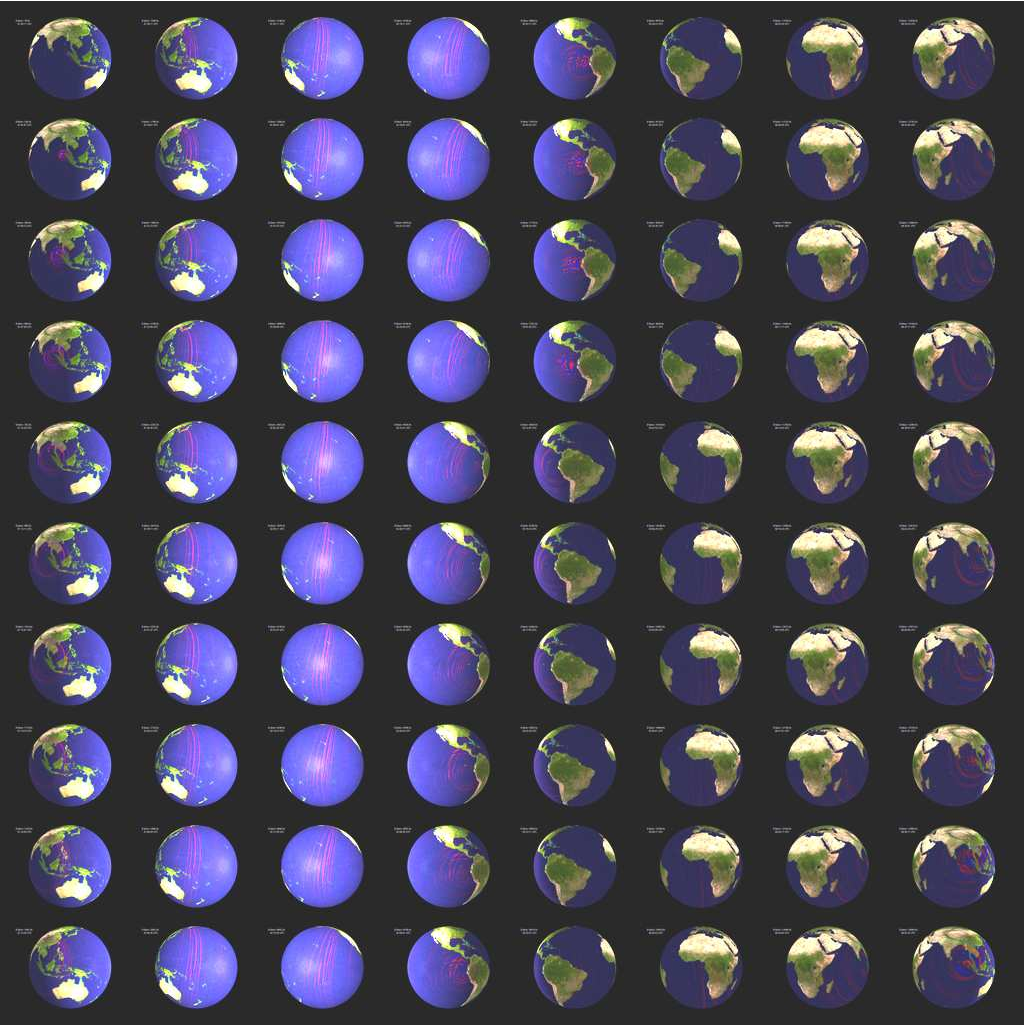
\includegraphics[scale=0.75]{figures/geo-poster4_small.pdf}
\par\end{centering}

\caption{Snapshots from a global movie for the December 26, 2004, M=9.2 Sumatra-Andaman
earthquake. Time runs down successive columns.}

\end{figure}



\subsection{Movie Volume}\label{sub:Movie-Volume}

When running xspecfem3D with the \texttt{\small MOVIE\_VOLUME} flag
turned on, the code outputs several files in \texttt{\small LOCAL\_DIR}.
As the files can be very large, there are several flags in the \texttt{\small Par\_file}
that control the region in space and time that is saved. These are:
\texttt{\small MOVIE\_TOP\_KM}, \texttt{\small MOVIE\_BOTTOM\_KM},
\texttt{\small MOVIE\_WEST\_DEG}, \texttt{\small MOVIE\_EAST\_DEG},
\texttt{\small MOVIE\_NORTH\_DEG}, \texttt{\small MOVIE\_SOUTH\_DEG},
\texttt{\small MOVIE\_START} and \texttt{\small MOVIE\_STOP}. The
code will save a given element if the center of the element is in
the prescribed volume.\newline


\begin{description}
\item [{The~Top/Bottom:}] Depth below the surface in kilometers, use \texttt{\small MOVIE\_TOP}
\texttt{\small =} \texttt{\small -100.0} to make sure the surface
is stored.
\item [{West/East:}] Longitude, degrees East {[}-180.0/180.0]
\item [{North/South:}] Latitute, degrees North {[}-90.0/90.0]
\item [{Start/Stop:}] Frames will be stored at \texttt{\small MOVIE\_START}
\texttt{\small +} \texttt{\small i{*}NSTEP\_BETWEEN\_FRAMES}, where
\texttt{\small i=(0,1,2..)} while \texttt{\small i{*}NSTEP\_BETWEEN\_FRAMES}
\texttt{\small <=} \texttt{\small MOVIE\_STOP}{\small \par}
\end{description}
The code saves several files, and the output is saved by each processor.
The first is \texttt{\small proc??????\_movie3D\_info.txt} which contains
two numbers, first the number of points within the prescribed volume
within this particular slice, and second the number of elements. The
next files are \texttt{\small proc??????\_movie3D\_x.bin}, \texttt{\small proc??????\_movie3D\_y.bin},
\texttt{\small proc??????\_movie3D\_z.bin} which store the locations
of the points in the 3D mesh.\newline


Finally the code stores the ``value'' at each of the points. Which
value is determined by \texttt{\small MOVIE\_VOLUME\_TYPE} in the
\texttt{\small Par\_file}. Choose 1 to save the strain, 2 to save
the time integral of strain, and 3 to save $\mu${*}time integral
of strain in the subvolume. Choosing 4 causes the code to save the
trace of the stress and the deviatoric stress in the whole volume
(not the subvolume in space), at the time steps specified. The name
of the output file will depend on the \texttt{\small MOVIE\_VOLUME\_TYPE}
chosen.\newline


Setting \texttt{\small MOVIE\_VOLUME\_COARSE} \texttt{\small =} \texttt{\small .true.}
will make the code save only the corners of the elements, not all
the points within each element for \texttt{\small MOVIE\_VOLUME\_TYPE}
\texttt{\small =} \texttt{\small 1,2,3}.\newline


To make the code output your favorite ``value'' simply add a new \texttt{\small MOVIE\_VOLUME\_TYPE},
a new subroutine to \texttt{\small write\_movie\_volume.f90} and a
subroutine call to \texttt{\small specfem3D.F90}.\newline


A utility program to combine the files produced by \texttt{\small MOVIE\_VOLUME\_TYPE}
\texttt{\small =} \texttt{\small 1,2,3} is provided in \texttt{\small combine\_paraview}~\\
\texttt{\small \_strain\_data.f90}. Type \texttt{\small xcombine\_paraview\_strain\_data}
to get the usage statement. The program \texttt{\small combine\_vol}~\\
\texttt{\small \_data.f90} can be used for \texttt{\small MOVIE\_VOLUME\_TYPE}
\texttt{\small =} \texttt{\small 4}.


\section{Finite-Frequency Kernels}\label{sec:Finite-Frequency-Kernels}

The finite-frequency kernels computed as explained in Section \ref{sec:Adjoint-simulation-finite}
are saved in the \texttt{LOCAL\_PATH} at the end of the simulation.
Therefore, we first need to collect these files on the front end,
combine them into one mesh file, and visualize them with some auxilliary
programs. Examples of kernel simulations may be found in the \texttt{EXAMPLES} directory.\newline


\begin{enumerate}
%%
\item \textbf{Create slice files}
%%

We will only discuss the case of one source-receiver pair, i.e., the
so-called banana-doughnut kernels. Although it is possible to collect
the kernel files from all slices onto the front end, it usually takes
up too much storage space (at least tens of gigabytes). Since the
sensitivity kernels are the strongest along the source-receiver great
circle path, it is sufficient to collect only the slices that are
along or close to the great circle path.\newline


A Perl script \texttt{utils/Visualization/VTK\_Paraview/global\_slice\_number.pl} can
help to figure out the slice numbers that lie along the great circle
path (both the minor and major arcs), as well as the slice numbers
required to produce a full picture of the inner core if your kernel
also illuminates the inner core.\newline

\begin{enumerate}
\item You need to first compile the utility programs provided in the \texttt{utils/Visualization/VTK\_Paraview/}~\\
\texttt{global\_slice\_util
}directory. Then copy the \texttt{CMTSOLUTION} file, \texttt{STATIONS\_ADJOINT},
and \texttt{Par\_file}, and run:
\begin{verbatim}
global_slice_number.pl CMTSOLUTION STATIONS_ADJOINT Par_file
\end{verbatim}
In the case of visualization boundary kernels or spherical cross-sections
of the volumetric kernels, it is necessary to obtain the slice numbers
that cover a belt along the source and receiver great circle path,
and you can use the hybrid version:
\begin{verbatim}
globe_slice_number2.pl CMTSOLUTION STATIONS _ADJOINT \
     Par_file belt_width_in_degrees
\end{verbatim}
A typical value for \texttt{belt\_width\_in\_degrees} can be 20.

\item For a full 6-chunk simulation, this script will generate the \texttt{slice\_minor},
\texttt{slice\_major}, \texttt{slice\_ic} files, but for a one-chunk simulation, this script only generates the \texttt{slice\_minor}
file.

\item For cases with multiple sources and multiple receivers, you need to
provide a slice file before proceeding to the next step.
\end{enumerate}

%%
\item \textbf{Collect the kernel files}
%%

After obtaining the slice files, you can collect the corresponding
kernel files from the given slices.

\begin{enumerate}
\item To accomplish this, you can use or modify the scripts in \texttt{utils/collect\_database} directory:
{\small
\begin{verbatim}
copy_m(oc,ic)_globe_database.pl slice_file lsf_machine_file filename [jobid]
\end{verbatim}
}
for volumetric kernels, where \texttt{\small lsf\_machine\_file} is
the machine file generated by the LSF scheduler, \texttt{\small filename}
is the kernel name (e.g., \texttt{\small rho\_kernel}, \texttt{\small alpha\_kernel}
and \texttt{\small beta\_kernel}), and the optional \texttt{\small jobid}
is the name of the subdirectory under \texttt{\small LOCAL\_PATH}
where all the kernel files are stored. For boundary kernels, you need
to use
{\small
\begin{verbatim}
copy_surf_globe_database.pl slice_file lsf_machine_file filename [jobid]
\end{verbatim}
}
where the filename can be \texttt{\small Moho\_kernel}, \texttt{\small d400\_kernel},
\texttt{\small d670\_kernel}, \texttt{\small CMB\_kernel} and \texttt{\small ICB\_kernel}.

\item After executing this script, all the necessary mesh topology files
as well as the kernel array files are collected to the local directory
on the front end.
\end{enumerate}

%%
\item \textbf{Combine kernel files into one mesh file}
%%

We use an auxiliary program \texttt{combine\_vol\_data.F90} to combine
the volumetric kernel files from all slices into one mesh file, and
\texttt{combine\_surf\_data.F90} to combine the surface kernel files.

\begin{enumerate}
\item Compile it in the global code directory:
{\footnotesize
\begin{verbatim}
make combine_vol_data
./bin/xcombine_vol_data slice_list kernel_filename input_topo_dir \
               input_file_dir output_dir low/high-resolution-flag-0-or-1 [region]
\end{verbatim}
}
%
where \texttt{input\_dir} is the directory where all the individual
kernel files are stored, and \texttt{output\_dir} is where the mesh
file will be written. Give 0 for low resolution and 1 for high resolution.
If region is not specified, all three regions (crust and mantle, outer core, inner core)
will be collected, otherwise, only the specified region will be.\newline

Here is an example:
{\footnotesize
\begin{verbatim}
./xcombine_vol_data slices_major alpha_kernel input_topo_dir input_file_dir output_dir 1
\end{verbatim}
}
For surface sensitivity kernels, use
{\footnotesize
\begin{verbatim}
./bin/xcombine_surf_data slice_list filename surfname input _dir output_dir low/high-resolution 2D/3D
\end{verbatim}
}
where \texttt{surfname} should correspond to the specific kernel file
name, and can be chosen from \texttt{Moho}, \texttt{400}, \texttt{670},
\texttt{CMB} and \texttt{ICB}.

\item Use 1 for a high-resolution mesh, outputting all the GLL points to
the mesh file, or use 0 for low resolution, outputting only the corner
points of the elements to the mesh file. Use 0 for 2D surface kernel
files and 1 for 3D volumetric kernel files.

\item Use region = 1 for the mantle, region = 2 for the outer core, region = 3 for the inner core, and region = 0 for all regions.

\item The output mesh file will have the name \texttt{reg\_?\_rho(alpha,beta)\_kernel.mesh,}
or\texttt{ }~\\
\texttt{reg\_?\_Moho(d400,d670,CMB,ICB)\_kernel.surf.}
\end{enumerate}

You can also use the binaries \texttt{xcombine\_vol\_data\_vtk} or \texttt{xcombine\_vol\_data\_vtu} with the same argument list
to directly output \texttt{.vtk} or \texttt{.vtu} files, respectively. This will make the following conversion step for \texttt{.mesh} files unnecessary.

\item \textbf{Convert mesh files into .vtu files}
\begin{enumerate}
\item We next convert the \texttt{.mesh} file into the VTU (Unstructured
grid file) format which can be viewed in ParaView, for example:
\begin{verbatim}
mesh2vtu -i file.mesh -o file.vtu
\end{verbatim}

\item Notice that this program \texttt{mesh2vtu}, in the
\texttt{utils/Visualization/VTK\_Paraview/mesh2vtu} directory, uses the
\href{http://www.vtk.org}{VTK} run-time library for its execution. Therefore,
make sure you have it properly installed.
\end{enumerate}

%%
\item \textbf{Copy over the source and receiver .vtk file}
%%

In the case of a single source and a single receiver, the simulation
also generates the \texttt{OUTPUT\_FILES/sr.vtk} file to describe
the source and receiver locations, which can be viewed in Paraview
in the next step.

%%
\item \textbf{View the mesh in ParaView}
%%

Finally, we can view the mesh in \href{http://www.paraview.org}{ParaView}.

\begin{enumerate}
\item Open ParaView.
\item From the top menu, \textsf{File} $\rightarrow$\textsf{ Open data},
select \texttt{file.vtu}, and click the \textsf{Accept} button.

\begin{itemize}
\item If the mesh file is of moderate size, it shows up on the screen; otherwise,
only the outline is shown.
\end{itemize}

\item Click \textsf{Display Tab} $\rightarrow$ \textsf{Display Style} $\rightarrow$
\textsf{Representation} and select \textsf{wireframe of surface} to
display it.

\item To create a cross-section of the volumetric mesh, choose \textsf{Filter}
$\rightarrow$ \textsf{cut}, and under \textsf{Parameters Tab}, choose
\textsf{Cut Function} $\rightarrow$ \textsf{plane}.

\item Fill in center and normal information given by the standard output
from \texttt{global\_slice\_number.pl} script.

\item To change the color scale, go to \textsf{Display Tab} $\rightarrow$
\textsf{Color} $\rightarrow$ \textsf{Edit Color Map} and reselect
lower and upper limits, or change the color scheme.

\item Now load in the source and receiver location file by \textsf{File}
$\rightarrow$\textsf{ Open data}, select \texttt{sr.vt}k, and click
the \textsf{Accept} button. Choose \textsf{Filter} $\rightarrow$\textsf{
Glyph}, and represent the points by `\textsf{spheres}'.

\item For more information about ParaView, see the \href{http://www.paraview.org/files/v1.6/ParaViewUsersGuide.PDF}{ParaView Users Guide}.
\end{enumerate}
\end{enumerate}
For illustration purposes, Figure \ref{fig:P-wave-speed-finite-frequency}
shows P-wave speed finite-frequency kernels from cross-correlation traveltime and amplitude measurements for a P arrival recorded at an epicentral distance of $60^{\circ}$ for a deep event.

%
\begin{figure}[H]
\noindent \begin{centering}
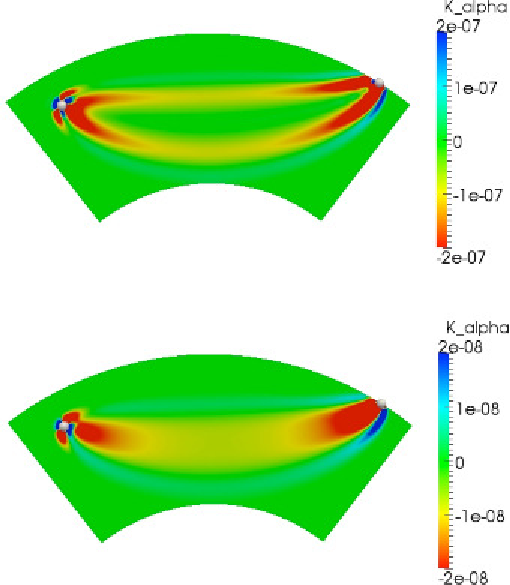
\includegraphics[clip,scale=1.2]{figures/P_alpha_60d_17s.pdf}
\caption{P-wave speed finite-frequency
kernels from cross-correlation traveltime (top) and amplitude (bottom) measurements
for a P arrival recorded at an epicentral distance of $60^{\circ}$.
The kernels together with the associated files and routines to reproduce them
may be found in \texttt{EXAMPLES/global\_PREM\_kernels/}.
}
\label{fig:P-wave-speed-finite-frequency}
\par\end{centering}
\end{figure}





\chapter{Running through a Scheduler}\label{cha:Running-Scheduler}

The code is usually run on large parallel machines, often PC clusters,
most of which use schedulers, i.e., queuing or batch management systems
to manage the running of jobs from a large number of users. The following
considerations need to be taken into account when running on a system
that uses a scheduler:\newline


\begin{itemize}
\item The processors/nodes to be used for each run are assigned dynamically
by the scheduler, based on availability. Therefore, in order for the
mesher and the solver (or between successive runs of the solver) to
have access to the same database files (if they are stored on hard
drives local to the nodes on which the code is run), they must be
launched in sequence as a single job.
\item On some systems, the nodes to which running jobs are assigned are
not configured for compilation. It may therefore be necessary to pre-compile
both the mesher and the solver. A small program provided in the distribution
called \texttt{\small create\_header\_file.f90} can be used to directly
create\texttt{\small{} OUTPUT\_FILES/values\_from\_mesher.h} using
the information in the \texttt{\small DATA/Par\_file} without having
to run the mesher (type \texttt{\small `make}{\small{} }\texttt{\small create\_header\_}~\\
\texttt{\small file}' to compile it and `\texttt{\small ./bin/xcreate\_header\_file}'
to run it; refer to the sample scripts below). The solver can now
be compiled as explained above.
\item One feature of schedulers/queuing systems is that they allow submission
of multiple jobs in a {}``launch and forget'' mode. In order to
take advantage of this property, care needs to be taken that output
and intermediate files from separate jobs do not overwrite each other,
or otherwise interfere with other running jobs.
\end{itemize}
We describe here in some detail a job submission procedure for the
Caltech 1024-node cluster, CITerra, under the LSF scheduling system.
We consider the submission of a regular forward simulation. The two
main scripts are \texttt{\small run\_lsf.bash}, which compiles the
Fortran code and submits the job to the scheduler, and \texttt{\small go\_mesher\_solver\_lsf}~\\
\texttt{\small .bash}, which contains the instructions that make up
the job itself. These scripts can be found in \texttt{\small utils/Cluster/lsf}
directory and can straightforwardly be modified and adapted to meet
more specific running needs.


\section{\texttt{run\_lsf.bash}}

This script first sets the job queue to be `normal'. It then compiles
the mesher and solver together, figures out the number of processors
required for this simulation from \texttt{DATA/Par\_file}, and submits
the LSF job.
{\small
\begin{verbatim}
#!/bin/bash
# use the normal queue unless otherwise directed queue="-q normal"
if [ $# -eq 1 ]; then
  echo"Setting the queue to $1"
  queue="-q $1"
fi
# compile the mesher and the solver
d=`date`
echo"Starting compilation $d"

make clean
make meshfem3D
make create_header_file

./bin/xcreate_header_file

make specfem3D

d=`date`
echo"Finished compilation $d"

# compute total number of nodes needed
NPROC_XI=`grep ^NPROC_XI DATA/Par_file | cut -c 34- `
NPROC_ETA=`grep ^NPROC_ETA DATA/Par_file | cut -c 34- `
NCHUNKS=`grep ^NCHUNKS DATA/Par_file | cut -c 34- `

# total number of nodes is the product of the values read
numnodes=$(( $NCHUNKS * $NPROC_XI * $NPROC_ETA ))

echo "Submitting job"
bsub $queue -n $numnodes -W 60 -K <go_mesher_solver_lsf_globe.bash
\end{verbatim}
}

\section{\texttt{go\_mesher\_solver\_lsf\_globe.bash}}

This script describes the job itself, including setup steps that can
only be done once the scheduler has assigned a job-ID and a set of
compute nodes to the job, the \texttt{run\_lsf.bash} commands used
to run the mesher and the solver, and calls to scripts that collect
the output seismograms from the compute nodes and perform clean-up
operations.

\begin{enumerate}
\item First the script directs the scheduler to save its own output and
output from \texttt{stdout} into \texttt{\small OUTPUT\_FILES/\%J.o},
where \texttt{\%J} is short-hand for the job-ID; it also tells the
scheduler what version of \texttt{mpich} to use (\texttt{mpich\_gm})
and how to name this job (\texttt{go\_mesher\_solver\_lsf}).
\item The script then creates a list of the nodes allocated to this job
by echoing the value of a dynamically set environment variable \texttt{LSB\_MCPU\_HOSTS}
and parsing the output into a one-column list using the Perl script
\texttt{utils/Cluster/lsf/remap\_lsf\_machines.pl}. It then creates a set of scratch
directories on these nodes (\texttt{\small /scratch/}~\\
\texttt{\small \$USER/DATABASES\_MPI}) to be used as the \texttt{LOCAL\_PATH}
for temporary storage of the database files. The scratch directories
are created using \texttt{shmux}, a shell multiplexor that can execute
the same commands on many hosts in parallel. \texttt{shmux} is available
from \href{http://web.taranis.org/shmux/}{Shmux}. Make sure that the \texttt{LOCAL\_PATH}
parameter in \texttt{DATA/Par\_file} is also set properly.
\item The next portion of the script launches the mesher and then the solver
using \texttt{run\_lsf.bash}.
\item The final portion of the script performs clean up on the nodes using
the Perl script \texttt{cleanmulti.pl}
\end{enumerate}
{\small
\begin{verbatim}
#!/bin/bash -v
#BSUB -o OUTPUT_FILES/%J.o
#BSUB -a mpich_gm
#BSUB -J go_mesher_solver_lsf

BASEMPIDIR=/scratch/$USER/DATABASES_MPI
echo "$LSB_MCPU_HOSTS" > OUTPUT_FILES/lsf_machines
echo "$LSB_JOBID" > OUTPUT_FILES/jobid

./remap_lsf_machines.pl OUTPUT_FILES/lsf_machines > OUTPUT_FILES/machines

# Modif : create a directory for this job
shmux -M50 -Sall \
 -c "mkdir -p /scratch/$USER;mkdir -p $BASEMPIDIR.$LSB_JOBID" - < OUTPUT_FILES/machines >/dev/null

# Set the local path in Par_file
sed -e "s:^LOCAL_PATH .*:LOCAL_PATH = $BASEMPIDIR.$LSB_JOBID:" < DATA/Par_file > DATA/Par_file.tmp
mv DATA/Par_file.tmp DATA/Par_file

current_pwd=$PWD

mpirun.lsf --gm-no-shmem --gm-copy-env $current_pwd/bin/xmeshfem3D
mpirun.lsf --gm-no-shmem --gm-copy-env $current_pwd/bin/xspecfem3D

# clean up
cleanbase_jobid.pl OUTPUT_FILES/machines DATA/Par_file
\end{verbatim}
}


\section{\texttt{run\_lsf.kernel} and \texttt{go\_mesher\_solver\_globe.kernel}}

For kernel simulations, you can use the sample run scripts \texttt{run\_lsf.kernel}
and \texttt{go\_mesher\_solver\_globe}~\\
\texttt{.kernel} provided in \texttt{utils/Cluster} directory, and modify
the command-line arguments of \texttt{xcreate\_adjsrc\_traveltime} in
\texttt{go\_mesher\_solver\_globe.kernel} according to the start and end time
of the specific portion of the forward seismograms you are interested
in.






\chapter{Changing the Model}\label{cha:-Changing-the}

In this section we explain how to change the crustal, mantle, or inner
core models. These changes involve contributing specific subroutines
that replace existing subroutines in the \texttt{SPECFEM3D\_GLOBE}
package.


\section{Changing the Crustal Model}\label{sec:Changing-the-Crustal}

The 3D crustal model Crust2.0 \citep{BaLaMa00} is superimposed onto
the mesh by the subroutine \texttt{model\_crust}~\\
\texttt{.f90}. To accomplish this, the flag \texttt{CRUSTAL}, set
in the subroutine \texttt{get\_model\_parameters.f90}, is used
to indicate a 3D crustal model. When this flag is set to \texttt{.true.},
the crust on top of the 1D reference model (PREM, IASP91, or AK135F\_NO\_MUD)
is removed and replaced by extending the mantle. The 3D crustal model
is subsequently overprinted onto the crust-less 1D reference model.
The call to the 3D crustal routine is of the form
\begin{verbatim}
call model_crust(lat,lon,r,vp,vs,rho,moho,foundcrust,CM_V,elem_in_crust)
\end{verbatim}

\noindent
Input to this routine consists of:
\begin{description}
\item [{\texttt{lat}}] Latitude in degrees.
\item [{\texttt{lon}}] Longitude in degrees.
\item [{\texttt{r}}] Non-dimensionalized radius ($0<\texttt{r}<1$).
\end{description}
%
Output from the routine consists of:
\begin{description}
\item [{\texttt{vp}}] Non-dimensionalized compressional wave speed at location
(\texttt{lat},\texttt{lon},\texttt{r}).
\item [{\texttt{vs}}] Non-dimensionalized shear wave speed.
\item [{\texttt{rho}}] Non-dimensionalized density.
\item [{\texttt{moho}}] Non-dimensionalized Moho depth.
\item [{\texttt{found\_crust}}] Logical that is set to \texttt{.true.}
only if crust exists at location (\texttt{lat},\texttt{lon},\texttt{r}),
i.e., \texttt{.false.} for radii \texttt{r} in the mantle. This flags
determines whether or not a particular location is in the crust and,
if so, what parameters to assign to the mesh at this location.
\item [{\texttt{CM\_V}}] Fortran structure that contains the parameters,
variables and arrays that describe the model.
\item [{\texttt{elem\_in\_crust}}] Logical that is used to force the
routine to return crustal values, even if the location would
be below the crust.
\end{description}
All output needs to be non-dimensionalized according to the convention
summarized in Appendix~\ref{cha:Non-Dimensionalization-Conventions}.
You can replace this subroutine by your own routine \textit{provided
you do not change the call structure of the routine}, i.e., the new
routine should take exactly the same input and produce the required,
properly non-dimensionalized output.

Part of the file \texttt{model\_crust.f90} is the subroutine \texttt{model\_crust\_broadcast}.
The call to this routine takes argument \texttt{CM\_V} and is used
to once-and-for-all read in the databases related to Crust2.0 and
broadcast the model to all parallel processes. If
you replace the file \texttt{model\_crust.f90} with your own implementation,
you \textit{must} provide a \texttt{model\_crust\_broadcast} routine,
even if it does nothing. Model constants and variables read by the
routine \texttt{model\_crust\_broadcast} are passed to the subroutine
\texttt{read\_crust\_model} through the structure \texttt{CM\_V}.
An alternative crustal model could use the same construct. Please
feel free to contribute subroutines for new models and send them to
us so that they can be included in future releases of the software.

\begin{quote}
\textbf{NOTE:} If you decide to create your own version of file \texttt{model\_crust.f90},
you must add calls to \texttt{MPI\_BCAST} in the subroutine \texttt{model\_crust\_broadcast}
after the call to the \texttt{read\_crust\_model} subroutine that
reads the isotropic mantle model once and for all in the mesher. This
is done in order to read the (potentially large) model data files
on the main node (which is the processor of rank 0 in our code)
only and then send a copy to all the other nodes using an MPI broadcast,
rather than using an implementation in which all the nodes would read
the same model data files from a remotely-mounted home file system,
which could create a bottleneck on the network in the case of a large
number of nodes. For example, in the current call to that routine
from \texttt{model\_crust.f90,} we write:

{\footnotesize
\begin{verbatim}
! the variables read are declared and stored in structure CM_V
  if(myrank == 0) call read_crust_model(CM_V)

! broadcast the information read on the main node to all the nodes
  call MPI_BCAST(CM_V%thlr,NKEYS_CRUST*NLAYERS_CRUST,MPI_DOUBLE_PRECISION,0,MPI_COMM_WORLD,ier)
  call MPI_BCAST(CM_V%velocp,NKEYS_CRUST*NLAYERS_CRUST,MPI_DOUBLE_PRECISION,0,MPI_COMM_WORLD,ier)
  call MPI_BCAST(CM_V%velocs,NKEYS_CRUST*NLAYERS_CRUST,MPI_DOUBLE_PRECISION,0,MPI_COMM_WORLD,ier)
  call MPI_BCAST(CM_V%dens,NKEYS_CRUST*NLAYERS_CRUST,MPI_DOUBLE_PRECISION,0,MPI_COMM_WORLD,ier)
  call MPI_BCAST(CM_V%abbreviation,NCAP_CRUST*NCAP_CRUST,MPI_CHARACTER,0,MPI_COMM_WORLD,ier)
  call MPI_BCAST(CM_V%code,2*NKEYS_CRUST,MPI_CHARACTER,0,MPI_COMM_WORLD,ier)
\end{verbatim}
}
\end{quote}

\section{Changing the Mantle Model}\label{sec:Changing-the-Mantle}

This section discusses how to change isotropic and anisotropic 3D
mantle models. Usually such changes go hand-in-hand with changing
the 3D crustal model.


\subsection{Isotropic Models}\label{sub:Isotropic-Models}

The 3D mantle model S20RTS \citep{RiVaWo99} is superimposed onto
the mantle mesh by the subroutine \texttt{model\_s20rts.f90}. The
call to this subroutine is of the form
\begin{verbatim}
call model_s20rts(radius,theta,phi,dvs,dvp,drho,D3MM_V)
\end{verbatim}

\noindent
Input to this routine consists of:
\begin{description}
\item [{\texttt{radius}}] Non-dimensionalized radius ($\texttt{RCMB/R\_ EARTH}<\texttt{r}<\texttt{RMOHO/R\_ EARTH}$;
for a given 1D reference model, the constants \texttt{RCMB} and \texttt{RMOHO}
are set in the \texttt{\small get\_model\_parameters}\texttt{.f90}
file). The code expects the isotropic mantle model to be defined between
the Moho (with radius \texttt{RMOHO} in m) and the core-mantle boundary
(CMB; radius \texttt{RCMB} in m) of a 1D reference model. When a 3D
crustal model is superimposed, as will usually be the case, the 3D
mantle model is stretched to fill any potential gap between the radius
of the Moho in the 1D reference model and the Moho in the 3D crustal
model. Thus, when the Moho in the 3D crustal model is shallower than
the Moho in the reference model, e.g., typically below the oceans,
the mantle model is extended to fill this gap.
\item [{\texttt{theta}}] Colatitude in radians.
\item [{\texttt{phi}}] Longitude in radians.
\end{description}
%
Output from the routine are the following non-dimensional perturbations:
\begin{description}
\item [{\texttt{dvs}}] Relative shear-wave speed perturbations $\delta\beta/\beta$
at location (\texttt{radius},\texttt{theta},\texttt{phi}).
\item [{\texttt{dvp}}] Relative compressional-wave speed perturbations
$\delta\alpha/\alpha$.
\item [{\texttt{drho}}] Relative density perturbations $\delta\rho/\rho$.
\item [{\texttt{D3MM\_V}}] Fortran structure that contains the parameters,
variables and arrays that describe the model.
\end{description}
You can replace the \texttt{model\_s20rts.f90} file with your own
version \textit{provided you do not change the call structure of the
routine}, i.e., the new routine should take exactly the same input
and produce the required relative output.

Part of the file \texttt{model\_s20rts.f90} is the subroutine
\texttt{model\_s20rts\_broadcast}.
The call to this routine takes argument\texttt{ D3MM\_V} and is used
to once-and-for-all read in the databases related to S20RTS. If you
replace the file \texttt{model\_s20rts.f90} with your own implementation,
you \textit{must} provide a \texttt{model\_s20rts\_broadcast} routine,
even if it does nothing. Model constants and variables read by the
routine \texttt{model\_s20rts\_broadcast} are passed to the subroutine
\texttt{read\_model\_s20rts} through the structure \texttt{D3MM\_V.}
An alternative mantle model should use the same construct.

\begin{quote}
\textbf{NOTE:} If you decide to create your own version of file \texttt{model\_s20rts.f90},
you must add calls to \texttt{MPI\_BCAST} in the subroutine \texttt{model\_s20rts\_broadcast}
after the call to the \texttt{read\_model\_s20rts} subroutine that
reads the isotropic mantle model once and for all in the mesher. This
is done in order to read the (potentially large) model data files
on the main node (which is the processor of rank 0 in our code)
only and then send a copy to all the other nodes using an MPI broadcast,
rather than using an implementation in which all the nodes would read
the same model data files from a remotely-mounted home file system,
which could create a bottleneck on the network in the case of a large
number of nodes. For example, in the current call to that routine
from \texttt{model\_s20rts.f90,} we write:

{\footnotesize
\begin{verbatim}
! the variables read are declared and stored in structure D3MM_V
  if(myrank == 0) call read_model_s20rts(D3MM_V)

! broadcast the information read on the main node to all the nodes
  call MPI_BCAST(D3MM_V%dvs_a,(NK+1)*(NS+1)*(NS+1),MPI_DOUBLE_PRECISION,0,MPI_COMM_WORLD,ier)
  call MPI_BCAST(D3MM_V%dvs_b,(NK+1)*(NS+1)*(NS+1),MPI_DOUBLE_PRECISION,0,MPI_COMM_WORLD,ier)
  call MPI_BCAST(D3MM_V%dvp_a,(NK+1)*(NS+1)*(NS+1),MPI_DOUBLE_PRECISION,0,MPI_COMM_WORLD,ier)
  call MPI_BCAST(D3MM_V%dvp_b,(NK+1)*(NS+1)*(NS+1),MPI_DOUBLE_PRECISION,0,MPI_COMM_WORLD,ier)
  call MPI_BCAST(D3MM_V%spknt,NK+1,MPI_DOUBLE_PRECISION,0,MPI_COMM_WORLD,ier)
  call MPI_BCAST(D3MM_V%qq0,(NK+1)*(NK+1),MPI_DOUBLE_PRECISION,0,MPI_COMM_WORLD,ier)
  call MPI_BCAST(D3MM_V%qq,3*(NK+1)*(NK+1),MPI_DOUBLE_PRECISION,0,MPI_COMM_WORLD,ier)
\end{verbatim}
}
\end{quote}


\subsection{Anisotropic Models}\label{sub:Anisotropic-Models}

Three-dimensional anisotropic mantle models may be superimposed on
the mesh based upon the subroutine
\begin{verbatim}
model_aniso_mantle.f90
\end{verbatim}
The call to this subroutine is of the form
\begin{verbatim}
call model_aniso_mantle(r,theta,phi,rho, &
         c11,c12,c13,c14,c15,c16,c22,c23,c24,c25,c26, &
         c33,c34,c35,c36,c44,c45,c46,c55,c56,c66,AMM_V)
\end{verbatim}

\noindent
Input to this routine consists of:
\begin{description}
\item [{\texttt{r}}] Non-dimensionalized radius ($\texttt{RCMB/R\_ EARTH}<\texttt{r}<\texttt{RMOHO/R\_ EARTH}$;
for a given 1D reference model, the constants \texttt{RCMB} and \texttt{RMOHO}
are set in the \texttt{\small get\_model\_parameters}\texttt{.f90}
file). The code expects the anisotropic mantle model to be defined
between the Moho and the core-mantle boundary (CMB). When a 3D crustal
model is superimposed, as will usually be the case, the 3D mantle
model is stretched to fill any potential gap between the radius of
the Moho in the 1D reference model and the Moho in the 3D crustal
model. Thus, when the Moho in the 3D crustal model is shallower than
the Moho in the reference model, e.g., typically below the oceans,
the mantle model is extended to fill this gap.
\item [{\texttt{theta}}] Colatitude in radians.
\item [{\texttt{phi}}] Longitude in radians.
\end{description}
%
Output from the routine consists of the following non-dimensional
model parameters:
\begin{description}
\item [{\texttt{rho}}] Non-dimensionalized density $\rho$.
\item [{\texttt{c11},}] \textbf{$\cdots$,} \texttt{\textbf{c66}} 21 non-dimensionalized
anisotropic elastic parameters.
\item [{\texttt{AMM\_V}}] Fortran structure that contains the parameters,
variables and arrays that describe the model.
\end{description}
You can replace the \texttt{model\_aniso\_mantle.f90} file by
your own version \textit{provided you do not change the call structure
of the routine}, i.e., the new routine should take exactly the same
input and produce the required relative output. Part of the file \texttt{model\_aniso\_mantle.f90}
is the subroutine \texttt{model\_aniso\_mantle\_broadcast}. The call to
this routine takes argument \texttt{AMM\_V} and is used to once-and-for-all
read in the static databases related to the anisotropic model. When
you choose to replace the file \texttt{model\_aniso\_mantle.f90}
with your own implementation you \textit{must} provide a \texttt{model\_aniso\_mantle\_broadcast}
routine, even if it does nothing. Model constants and variables read
by the routine \texttt{model\_aniso\_mantle\_broadcast} are passed through the
structure \texttt{AMM\_V}. An alternative anisotropic mantle model
should use the same construct.

\begin{quote}
\textbf{NOTE:} If you decide to create your own version of file \texttt{model\_aniso\_mantle.f90},
you must add calls to \texttt{MPI\_BCAST} in file \texttt{model\_aniso\_mantle.f90}
after the call to the \texttt{read\_aniso\_mantle\_model} subroutine
that reads the anisotropic mantle model once and for all in the mesher.
This is done in order to read the (potentially large) model data files
on the main node (which is the processor of rank 0 in our code)
only and then send a copy to all the other nodes using an MPI broadcast,
rather than using an implementation in which all the nodes would read
the same model data files from a remotely-mounted home file system,
which could create a bottleneck on the network in the case of a large
number of nodes. For example, in the current call to that routine
from \texttt{model\_aniso\_mantle.f90,} we write:

{\footnotesize
\begin{verbatim}
! the variables read are declared and stored in structure AMM_V
  if(myrank == 0) call read_aniso_mantle_model(AMM_V)

! broadcast the information read on the main node to all the nodes
  call MPI_BCAST(AMM_V%npar1,1,MPI_INTEGER,0,MPI_COMM_WORLD,ier)
  call MPI_BCAST(AMM_V%beta,14*34*37*73,MPI_DOUBLE_PRECISION,0,MPI_COMM_WORLD,ier)
  call MPI_BCAST(AMM_V%pro,47,MPI_DOUBLE_PRECISION,0,MPI_COMM_WORLD,ier)
\end{verbatim}
}
\end{quote}

Rotation of the anisotropic tensor elements from one coordinate system
to another coordinate system may be accomplished based upon the subroutine
\texttt{rotate\_aniso\_tensor}. Use of this routine requires understanding
the coordinate system used in \texttt{SPECFEM3D\_GLOBE}, as discussed
in Appendix~\ref{cha:Reference-Frame-Convention}.


\subsection{Point-Profile Models}\label{sub:Point-Profile-Models}

In order to facilitate the use of your own specific mantle model, you can choose \texttt{PPM} as model in the \texttt{DATA/Par\_file} file
and supply your own model as an ASCII-table file. These generic models are given as depth profiles at a specified lon/lat location
and a perturbation (in percentage) with respect to the shear-wave speed values from PREM. The ASCII-file should have a format like:

{\footnotesize
\begin{verbatim}
#lon(deg), lat(deg), depth(km), Vs-perturbation wrt PREM(%), Vs-PREM (km/s)
 -10.00000       31.00000       40.00000      -1.775005       4.400000
 -10.00000       32.00000       40.00000      -1.056823       4.400000
 ...
\end{verbatim}
}
\noindent
where the first line is a comment line and all following ones are specifying the Vs-perturbation at a lon/lat location and a given depth.
The last entry on each line is specifying the absolute value of Vs (however this value is only given as a supplementary information
and not used any further). The background model is PREM with a transverse isotropic layer between Moho and 220~km depth.
The specified Vs-perturbations are added as isotropic perturbations. Please see the file \texttt{DATA/PPM/README}
for more informations how to setup the directory \texttt{DATA/PPM} to use your own ASCII-file.



To change the code behavior of these PPM-routines, please have a look at the implementation in the source code
file \texttt{model\_ppm.f90} and set the flags and scaling factors as needed for your purposes.
Perturbations in density and Vp may be scaled to the given Vs-perturbations with constant scaling factors by setting the appropriate
values in this source code file. In case you want to change the format of the input ASCII-file, see more details in the Appendix \ref{cha:Troubleshooting}.




\section{Anelastic Models}\label{sec:Anelastic-Models}

Three-dimensional anelastic (attenuation) models may be superimposed
onto the mesh based upon your subroutine .
\texttt{model\_atten3D.f90}.
The call to this routine would be as follows
\begin{verbatim}
call model_atten3D(radius, colatitude, longitude, Qmu, QRFSI12_Q, idoubling)
\end{verbatim}

\noindent
Input to this routine consists of:
\begin{description}
\item [{\texttt{radius}}] scaled radius of the earth: $0\,(\mathrm{center})<=r\,<=1$(surface)
\item [{\texttt{latitude}}] Colatitude in degrees: $0^{\circ}<=\theta<=180^{\circ}$
\item [{\texttt{longitude}}] Longitude in degrees: $-180^{\circ}<=\phi<=180^{\circ}$
\item [{\texttt{QRFSI12\_Q}}] Fortran structure that contains the parameters,
variables and arrays that describe the model
\item [{\texttt{idoubling}}] value of the doubling index flag in each radial region of the mesh
\end{description}
%
Output to this routine consists of:
\begin{description}
\item [{\texttt{Qmu}}] Shear wave quality factor: $0<Q_{\mu}<5000$
\end{description}
A 3-D attenuation model QRFSI12 \citep{DaEkDz08}
is provided, as well as 1-D models with a PREM and a 1DREF
attenuation structure. By default the PREM attenuation model is taken,
using the routine \texttt{model\_attenuation\_1D\_PREM},
found in \texttt{model\_attenuation.f90}.

To create your own three-dimensional attenuation model, you add your model
using a routine like the ~\\
\texttt{model\_atten3D\_QRFSI12} subroutine
and the example routine above as a guide and replace the call in file
\texttt{meshfem3D\_models.f90} to your own subroutine.

Note that the resolution and maximum value of anelastic models are
truncated. This speeds the construction of the standard linear solids
during the meshing stage. To change the resolution, currently at one
significant figure following the decimal, or the maximum value (5000),
consult \texttt{constants.h}. In order to prevent unexpected results,
quality factors $Q_{\mu}$ should never be equal to 0 outside of the
inner core.





\chapter{Post-Processing Scripts}

Several post-processing scripts/programs are provided in the \texttt{utils/seis\_process}
directory, most of which need to be adjusted for different
systems, for example, the path of the executable programs. Here we
only list the available scripts and provide a brief description, and
you can either refer to the related sections for detailed usage or,
in many cases, type the script/program name without arguments
to see its usage.


\section{Clean Local Database}

After all the simulations are done, you may need to clean the local
scratch disks for the next simulation. This is especially important
in the case of 1- or 2-chunk kernel simulations, where very large files
are generated for the absorbing boundaries to help with the reconstruction
of the regular forward wavefield. A sample script is provided in \texttt{utils/Cluster/lsf}:
\begin{verbatim}
cleanbase.pl machines
\end{verbatim}

\section{Process Data and Synthetics}\label{sec:Process-data-and-syn}

In many cases, the SEM synthetics are calculated and compared to observed
seismograms recorded at seismic stations. Since the SEM synthetics
are accurate for a certain frequency range, both the original data
and the synthetics need to be processed before a comparison can be
made. For such comparisons, the following steps are recommended:\newline

\begin{enumerate}
\item Make sure that both synthetic and observed seismograms have the correct station/event and timing information.
\item Convolve synthetic seismograms with a source-time function with the half duration specified in the \texttt{CMTSOLUTION} file, provided, as recommended, you used a zero half duration in the SEM simulations.
\item Resample both observed and synthetic seismograms to a common sampling rate.
\item Cut the records using the same window.
\item Remove the trend and mean from the records and taper them.
\item Remove the instrument response from the observed seismograms (recommended) or convolve the synthetic seismograms with the instrument response.
\item Make sure that you apply the same filters to both observed and synthetic seismograms. Preferably, avoid filtering your records more than once.
\item Now, you are ready to compare your synthetic and observed seismograms.
\end{enumerate}

We generally use the following scripts for processing:

\subsection{\texttt{process\_data.pl}}

This script cuts a given portion of the original data, filters it,
transfers the data into a displacement record, and picks the first
P and S arrivals. For more functionality, type `\texttt{process\_data.pl}'
without any argument. An example of the usage of the script:

{\footnotesize
\begin{verbatim}
process_data.pl -m CMTSOLUTION -s 1.0 -l 0/4000 -i -f -t 40/500 -p -x bp DATA/1999.330*.LH?.SAC
\end{verbatim}
}

\noindent
which has resampled the SAC files to a sampling rate of 1 seconds, cut them between 0 and 4000 seconds, transfered them into displacement
records and filtered them between 40 and 500 seconds, picked the first P and S arrivals, and added suffix `\texttt{bp}' to the file names.\newline


Note that all of the scripts in this section actually use SAC,
saclst and/or IASP91 to do the core operations; therefore make sure
that the SAC, saclst and IASP91 packages are installed on your
system, and that all the environment variables are set properly before
running these scripts.


\subsection{\texttt{process\_syn.pl}}\label{sub:process_syn.pl}

This script converts the synthetic output from the SEM code from ASCII
to SAC format, and performs similar operations as `\texttt{process\_data.pl}'.
An example of the usage of the script:

{\footnotesize
\begin{verbatim}
process_syn.pl -m CMTSOLUTION -h -a STATIONS -s 1.0 -l 0/4000 -f -t 40/500 -p -x bp SEM/*.MX?.sem
\end{verbatim}
}

\noindent
which will convolve the synthetics with a triangular source-time function
from the \texttt{CMTSOLUTION} file, convert the synthetics into SAC
format, add event and station information into the SAC headers, resample the SAC files with a sampling rate of 1 seconds, cut them between 0 and 4000 seconds, filter them between 40 and
500 seconds with the same filter used for the observed data, pick the first P and S arrivals, and add the suffix `\texttt{bp}'
to the file names.\newline


More options are available for this script, such as adding a time shift
to the origin time of the synthetics, convolving the synthetics with
a triangular source-time function with a given half duration, etc.
Type \texttt{process\_syn.pl} without any argument for detailed
usage.


\subsection{\texttt{rotate.pl}}

To rotate the horizontal components of both the data and the synthetics
(i.e., \texttt{MXN} and \texttt{MXE}) to the transverse and radial directions (i.e., \texttt{MXT} and \texttt{MXR}),\texttt{\small{}
}use{\small{} }\texttt{\small rotate.pl}:\\

\noindent
data example:
\begin{verbatim}
rotate.pl -l 0 -L 4000 -d DATA/*.LHE.SAC.bp
\end{verbatim}
synthetics example:
\begin{verbatim}
rotate.pl -l 0 -L 4000 SEM/*.MXE.sem.sac.bp
\end{verbatim}

\noindent
where the first command performs rotation on the SAC data obtained
through IRIS (which may have timing information written in the filename),
while the second command rotates the processed synthetics.\newline


For synthetics, another (simpler) option is to set flag \texttt{ROTATE\_SEISMOGRAMS\_RT}
to \texttt{.true.} in the parameter file \texttt{DATA/Par\_file}.


\subsection{\texttt{clean\_sac\_headers\_after\_crash.sh}}

Note: You need to have the \texttt{sismoutil-0.9b} package installed
on your computer if you want to run this script on binary SAC files.
The software is available via the \href{http://www.orfeus-eu.org}{ORFEUS web site}.\newline


In case the simulation crashes during run-time without computing and
writing all time steps, the SAC files (if flags \texttt{OUTPUT\_SEISMOS\_SAC\_ALPHANUM}
or \texttt{OUTPUT\_SEISMOS\_SAC\_BINARY} have been set to \texttt{.true.})
are corrupted and cannot be used in SAC. If the simulation
ran long enough so that the synthetic data may still be of use, you
can run the script called \texttt{clean\_sac\_headers\_after\_crash.sh}
(located in the \texttt{utils/} directory) on the SAC files to correct
the header variable NPTS to the actually written number of time steps.
The script must be called from the \texttt{SPECFEM3D} main directory,
and the input argument to this script is simply a list of SAC seismogram
files.


\section{Map Local Database}

A sample program \texttt{remap\_database} is provided to map the local
database from a set of machines to another set of machines. This is
especially useful when you want to run mesher and solver, or different
types of solvers separately through a scheduler (refer to Chapter~\ref{cha:Running-Scheduler}).
\begin{verbatim}
run_lsf.bash --gm-no-shmem --gm-copy-env remap_database \
  old_machines 150 [old_jobid new_jobid]
\end{verbatim}
where \texttt{old\_machines} is the LSF machine file used in the previous
simulation, and \texttt{150} is the number of processors in total.
Note that you need to supply \texttt{old\_jobid} and \texttt{new\_jobid(\%J)}
which are the LSF job-IDs for the old and new run if your databases
are stored in a sub-directory named after the jobid on the scratch
disk.






%------------------------------------------------------------------------------------------------%

\chapter{Information for developers of the code, and for people who want to learn how the technique works}\label{cha:developers}

%------------------------------------------------------------------------------------------------%

You can get a very simple 1D version of a demo code (there is one in Fortran and one in Python):
\begin{verbatim}
git clone --recursive https://github.com/SPECFEM/specfem1d.git
\end{verbatim}

\noindent We also have simple 3D demo source codes that implement the SEM in a single, small program, in directory\\
utils/small\_SEM\_solvers\_in\_Fortran\_and\_C\_without\_MPI\_to\_learn of the specfem3d package.
They are useful to learn how the spectral-element method works, and how to write or modify a code to implement it.
Also useful to test new ideas by modifying these simple codes to run some tests.
We also have a similar, even simpler, demo source code for the 2D case in directory\\
utils/small\_SEM\_solver\_in\_Fortran\_without\_MPI\_to\_learn of the specfem2d package.

\noindent For information on how to contribute to the code, i.e., for how to make your modifications, additions or improvements part of the
official package, see \url{https://github.com/SPECFEM/specfem3d/wiki} .



\chapter*{Simulation features supported in SPECFEM3D\_GLOBE}
\addcontentsline{toc}{chapter}{Simulation features supported in SPECFEM3D\_GLOBE}

The following lists all available features for a SPECFEM3D\_GLOBE simulation,
where {\it CPU}, {\it CUDA} and {\it OpenCL} denote the code versions for CPU-only simulations,
CUDA and OpenCL hardware support, respectively.
%
\begin{table}[htp]
\label{table:features}
\begin{center}
\begin{tabular}{ l l c c c}
\hline
%{\bf Feature}    &   & \multicolumn{3}{c}{{\bf Code version}} \\
%\cmidrule(lr){3-5}
%           &     & {\it CPU} & {\it CUDA}  & {\it OpenCL} \\
%% to have proper title w/ pandoc
{\bf Feature}   &   & {\it CPU} & {\it CUDA}  & {\it OpenCL} \\
\hline
& & & & \\
%%
{\bf Physics}       & Ocean load      & X   & X   & X \\
                & Ellipticity               & X   & X       & X \\
                & Topography        & X       & X       & X \\
                & Gravity               & X       & X       & X \\
                & Rotation              & X       & X       & X \\
                & Attenuation       & X       & X       & X \\
\hline
& & & & \\
%%
{\bf Simulation Setup}  & Global (6-chunks)     & X & X & X \\
                  & Regional (1,2-chunk)    & X & X & X \\
                  & Restart/Checkpointing & X & X & X \\
                  & Simultaneous runs     & X & X & X \\
                  & ADIOS file I/O        & X & X & X \\
\hline
& & & & \\
%%
{\bf Sensitivity kernels} & Partial physical dispersion     & X     & X     & X \\
                  & Undoing of attenuation          & X     & X     & X \\
                  & Anisotropic kernels               & X     & X     & X \\
                  & Transversely isotropic kernels    & X     & X     & X \\
                  & Isotropic kernels             & X     & X     & X \\
                  & Approximate Hessian           & X     & X     & X \\
\hline
& & & & \\
%%
{\bf Time schemes}      & Newmark     & X     & X     & X \\
                    & LDDRK     & X     & -     & - \\
\hline
& & & & \\
%%
{\bf Visualization}     & Surface movie   & X     & X     & X \\
                  & Volumetric movie  & X     & X     & X \\
\hline
& & & & \\
%%
{\bf Seismogram formats}  & Ascii           & X   & X   & X \\
                    & SAC       & X & X & X \\
                    & ASDF      & X & X & X \\
                    & Binary      & X & X & X \\
%
\hline
& & & & \\ % to avoid clashes with pandoc
\end{tabular}
\end{center}
\end{table}




\chapter*{Bug Reports and Suggestions for Improvements}\label{cha:Bug-Reports-and}
\addcontentsline{toc}{chapter}{Bug Reports and Suggestions for Improvements}

To report bugs or suggest improvements to the code, please use the {\it Issues} feature on the github repository.



\chapter*{Notes and Acknowledgements}\label{cha:Notes-and-Acknowledgements}
\addcontentsline{toc}{chapter}{Notes and Acknowledgements}

In order to keep the software package thread-safe in case a multithreaded
implementation of MPI is used, developers should not add modules or
common blocks to the source code but rather use regular subroutine
arguments (which can be grouped in ``derived types'' if needed for
clarity).\newline


The Gauss-Lobatto-Legendre subroutines in \texttt{gll\_library.f90}
are based in part on software libraries from the Massachusetts Institute
of Technology, Department of Mechanical Engineering (Cambridge, Massachusetts, USA).
The non-structured global numbering software was provided by Paul
F. Fischer (Brown University, Providence, Rhode Island, USA, now at Argonne National Laboratory, USA).\newline


\href{http://www.opendx.org}{OpenDX} is open-source based on IBM Data Explorer,
\href{http://www.avs.com}{AVS} is a trademark of Advanced Visualization Systems,
and \href{http://www.paraview.org}{ParaView} is an open-source visualization
platform.{\small{} }{\small \par}


Please provide your feedback, questions, comments, and suggestions through the github repository.




\chapter*{Copyright}\label{cha:Copyright}
\addcontentsline{toc}{chapter}{Copyright}

Main `historical' authors: Dimitri Komatitsch and Jeroen Tromp (there are now many more!).

Princeton University, USA, and CNRS / University of Marseille, France.\\
$\copyright$ Princeton University, USA and CNRS / University of Marseille, France, April 2014\\

\noindent
This program is free software; you can redistribute it and/or modify
it under the terms of the GNU General Public License as published
by the Free Software Foundation (see Appendix \ref{cha:License}).\\

\noindent
Please note that by contributing to this code, the developer understands and agrees that this project and contribution
are public and fall under the open source license mentioned above.\\

\noindent
\textbf{\underline{Evolution of the code:}}\\

 v. 7.0, many developers, January 2015:
     simultaneous MPI runs, ADIOS file I/O support, ASDF seismograms, new seismogram names, tomography tools,
     CUDA and OpenCL GPU support, CEM model support, updates AK135 model, binary topography files,
     fixes geocentric/geographic conversions, updates ellipticity and gravity factors, git versioning system.\\

 v. 6.0, Daniel Peter (ETH Z\"urich, Switzerland), Dimitri Komatitsch and Zhinan Xie (CNRS / University of Marseille, France),
     Elliott Sales de Andrade (University of Toronto, Canada), and many others, in particular from Princeton University, USA,
     April 2014:
     more flexible MPI implementation, GPU support, exact undoing of attenuation, LDDRK4-6 higher-order time scheme, etc...\\

 v. 5.1, Dimitri Komatitsch, University of Toulouse, France and Ebru Bozdag, Princeton University, USA, February 2011:
     non blocking MPI for much better scaling on large clusters;
     new convention for the name of seismograms, to conform to the IRIS standard;
     new directory structure.\\

 v. 5.0, many developers, February 2010:
     new Moho mesh stretching honoring crust2.0 Moho depths,
     new attenuation assignment, new SAC headers, new general crustal models,
     faster performance due to Deville routines and enhanced loop unrolling,
     slight changes in code structure (see also trivia at program start).\\

 v. 4.0 David Mich\'ea and Dimitri Komatitsch, University of Pau, France, February 2008:
      first port to GPUs using CUDA, new doubling brick in the mesh, new perfectly load-balanced mesh,
      more flexible routines for mesh design, new inflated central cube
      with optimized shape, far fewer mesh files saved by the mesher,
      global arrays sorted to speed up the simulation, seismograms can be
      written by the main process, one more doubling level at the bottom
      of the outer core if needed (off by default).\\

 v. 3.6 Many people, many affiliations, September 2006:
      adjoint and kernel calculations, fixed IASP91 model,
      added AK135F\_NO\_MUD and 1066a, fixed topography/bathymetry routine,
      new attenuation routines, faster and better I/Os on very large
      systems, many small improvements and bug fixes, new `configure'
      script, new Pyre version, new user's manual etc..\\

 v. 3.5 Dimitri Komatitsch, Brian Savage and Jeroen Tromp, Caltech, July 2004:
      any size of chunk, 3D attenuation, case of two chunks,
      more precise topography/bathymetry model, new Par\_file structure.\\

 v. 3.4 Dimitri Komatitsch and Jeroen Tromp, Caltech, August 2003:
      merged global and regional codes, no iterations in fluid, better movies.\\

 v. 3.3 Dimitri Komatitsch, Caltech, September 2002:
      flexible mesh doubling in outer core, inlined code, OpenDX support.\\

 v. 3.2 Jeroen Tromp, Caltech, July 2002:
      multiple sources and flexible PREM reading.\\

 v. 3.1 Dimitri Komatitsch, Caltech, June 2002:
      vectorized loops in solver and merged central cube.\\

 v. 3.0 Dimitri Komatitsch and Jeroen Tromp, Caltech, May 2002:
   ported to SGI and Compaq, double precision solver, more general anisotropy.\\

 v. 2.3 Dimitri Komatitsch and Jeroen Tromp, Caltech, August 2001:
                       gravity, rotation, oceans and 3-D models.\\

 v. 2.2 Dimitri Komatitsch and Jeroen Tromp, Caltech, USA, March 2001:
                       final MPI package.\\

 v. 2.0 Dimitri Komatitsch, Harvard, USA, January 2000: MPI code for the globe.\\

 v. 1.0 Dimitri Komatitsch, UNAM, Mexico, June 1999: first MPI code for a chunk.\\

 Jeroen Tromp and Dimitri Komatitsch, Harvard, USA, July 1998: first chunk solver using OpenMP on a Sun machine.\\

 Dimitri Komatitsch, IPG Paris, France, December 1996: first 3-D solver for the CM-5 Connection Machine,
    parallelized on 128 processors using Connection Machine Fortran.\\



%%%%%%%%%%%%%%%%%%%%%%%%%%%%%%%%%%%%%%%%%%%
%% Bibliography
%%%%%%%%%%%%%%%%%%%%%%%%%%%%%%%%%%%%%%%%%%%

\bibliography{bibliography}

%%%%%%%%%%%%%%%%%%%%%%%%%%%%%%%%%%%%%%%%%%%
%% Appendix
%%%%%%%%%%%%%%%%%%%%%%%%%%%%%%%%%%%%%%%%%%%

\appendix
%dummy comment inserted by tex2lyx to ensure that this paragraph is not empty

\chapter{Reference Frame Convention}\label{cha:Reference-Frame-Convention}

The code uses the following convention for the Cartesian reference frame:

\begin{itemize}
\item the $x$ axis points East
\item the $y$ axis points North
\item the $z$ axis points up
\end{itemize}
Note that this convention is different from both the \citet{AkRi80}
convention and the Harvard Centroid-Moment Tensor (CMT) convention.
The Aki \& Richards convention is

\begin{itemize}
\item the $x$ axis points North
\item the $y$ axis points East
\item the $z$ axis points down
\end{itemize}
and the Harvard CMT convention is

\begin{itemize}
\item the $x$ axis points South
\item the $y$ axis points East
\item the $z$ axis points up
\end{itemize}





\chapter{Non-Dimensionalization Conventions}\label{cha:Non-Dimensionalization-Conventions}

All physical parameters used are non-dimensionalized internally in the code
in order to work in a reference Earth of radius 1. In Table~{\small \ref{table:conventions} in the right column are the values by which
we divide the parameters of the left column internally to perform the calculations.
The values output and saved by the code (seismograms, sensitivity kernels...) are then
scaled back to the right physical dimensions before being saved.
}%
\begin{table}[ht]
\noindent
\begin{centering}
{\small }\begin{tabular}{|c|c|}
\hline
quantity (units)  & divided internally by \\
\hline
distance (m)  & \texttt{R\_EARTH} \\
time (s)  & $1/\sqrt{\texttt{PI}\times\texttt{GRAV}\times\texttt{RHOAV}}$ \\
density (kg/m$^{3}$)  & \texttt{RHOAV} \\
\hline
\end{tabular}
\par
\end{centering}{\small \par}

\caption{Non-dimensionalization convention employed internally by the code. The constants \texttt{R\_EARTH}
(the radius of the Earth), \texttt{PI} (the number $\pi$), \texttt{GRAV}
(the universal gravitational constant), and \texttt{RHOAV} (the Earth's
average density) are defined in the \texttt{constants.h} file. }

{\small \label{table:conventions} }
\end{table}
{\small \par}




\chapter{Benchmarks}

\citet{KoTr02a,KoTr02b} carefully benchmarked the spectral-element
simulations of global seismic waves against normal-mode seismograms.
Version 4.0 of \texttt{SPECFEM3D\_GLOBE} has been benchmarked again
following the same procedure.\newline


In this appendix we present two tests: a `long-period' (periods longer
than 17~s) simulation of a shallow event in isotropic PREM \citep{DzAn81}
without the ocean layer, without attenuation but including the effects
of self-gravitation (in the Cowling approximation) (Figures \ref{fig:Vanuatu-with-Vertical}
and \ref{fig:Vanuatu-with-Transverse}), and a `short-period' (periods
longer than 9~s) simulation of a deep event in transversely isotropic
PREM without the ocean layer and including the effects of self-gravitation
and attenuation (Figures \ref{fig:Bolivia-with-Vertical}, \ref{fig:Bolivia-with-Transverse}
and \ref{fig:Bolivia-PKP}).

%
\begin{figure}[ht]
\noindent \begin{centering}
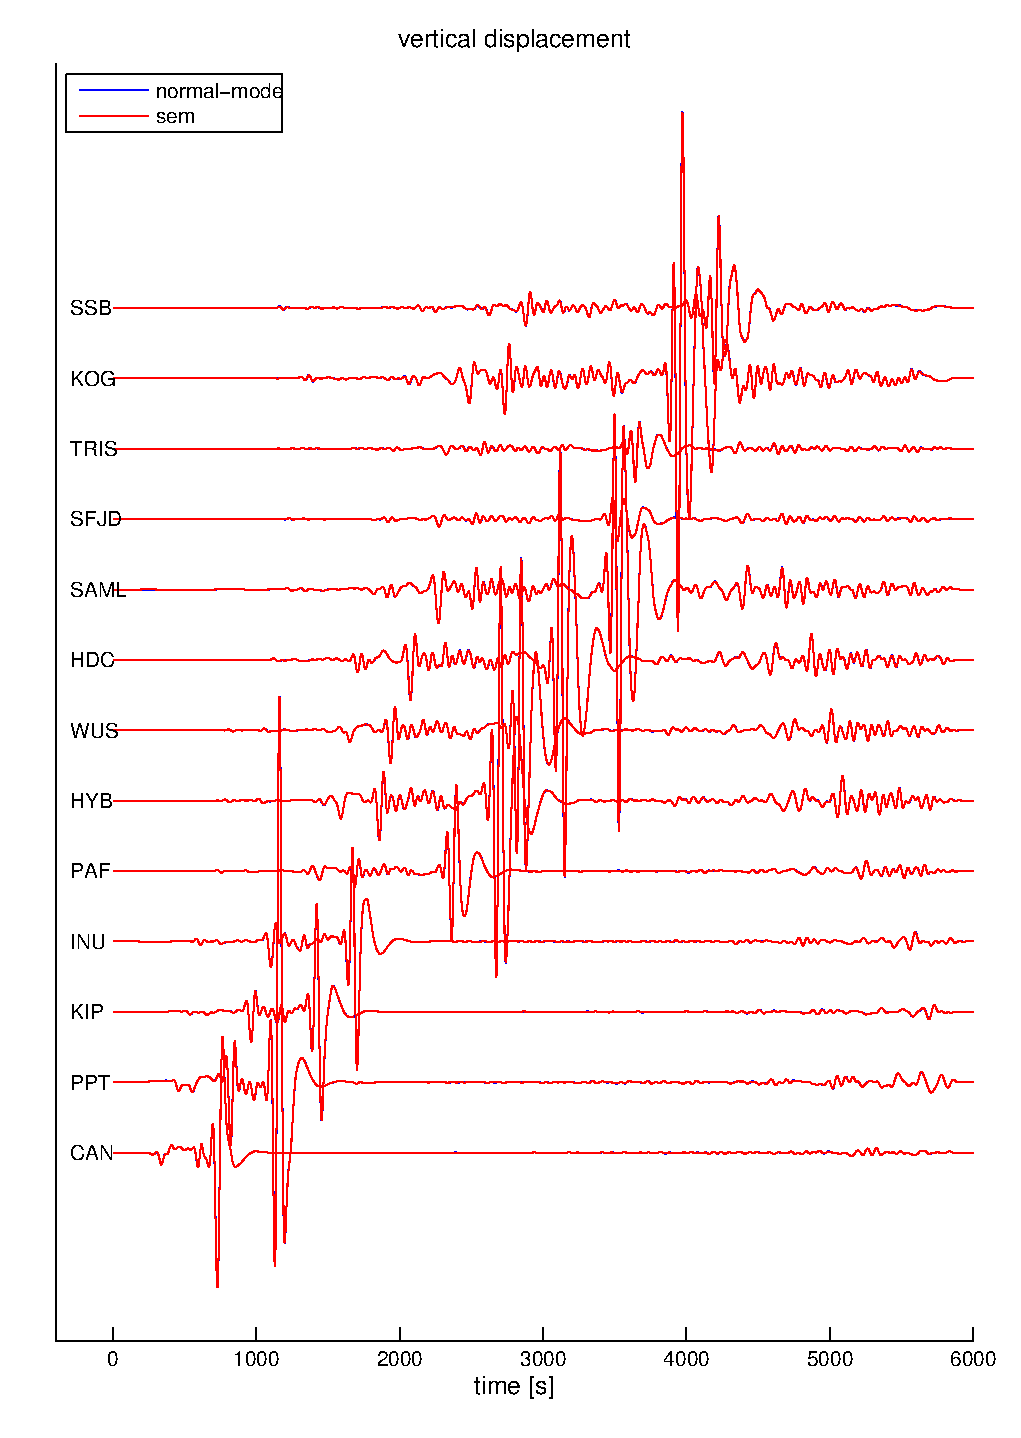
\includegraphics[scale=0.75]{figures/vanuatu_vertical.pdf}
\caption{Normal-mode (blue) and SEM (red)
vertical displacements in isotropic PREM considering the effects of
self-gravitation but not attenuation for 13 stations at increasing
distance from the 1999 November 26th Vanuatu event located at 15~km
depth. The SEM computation is accurate for periods longer than 17~s.
The seismograms have been filtered between 50~s and 500~s. The station
names are indicated on the left. }
\label{fig:Vanuatu-with-Vertical}

\par\end{centering}
\end{figure}
%
\begin{figure}[ht]
\noindent \begin{centering}
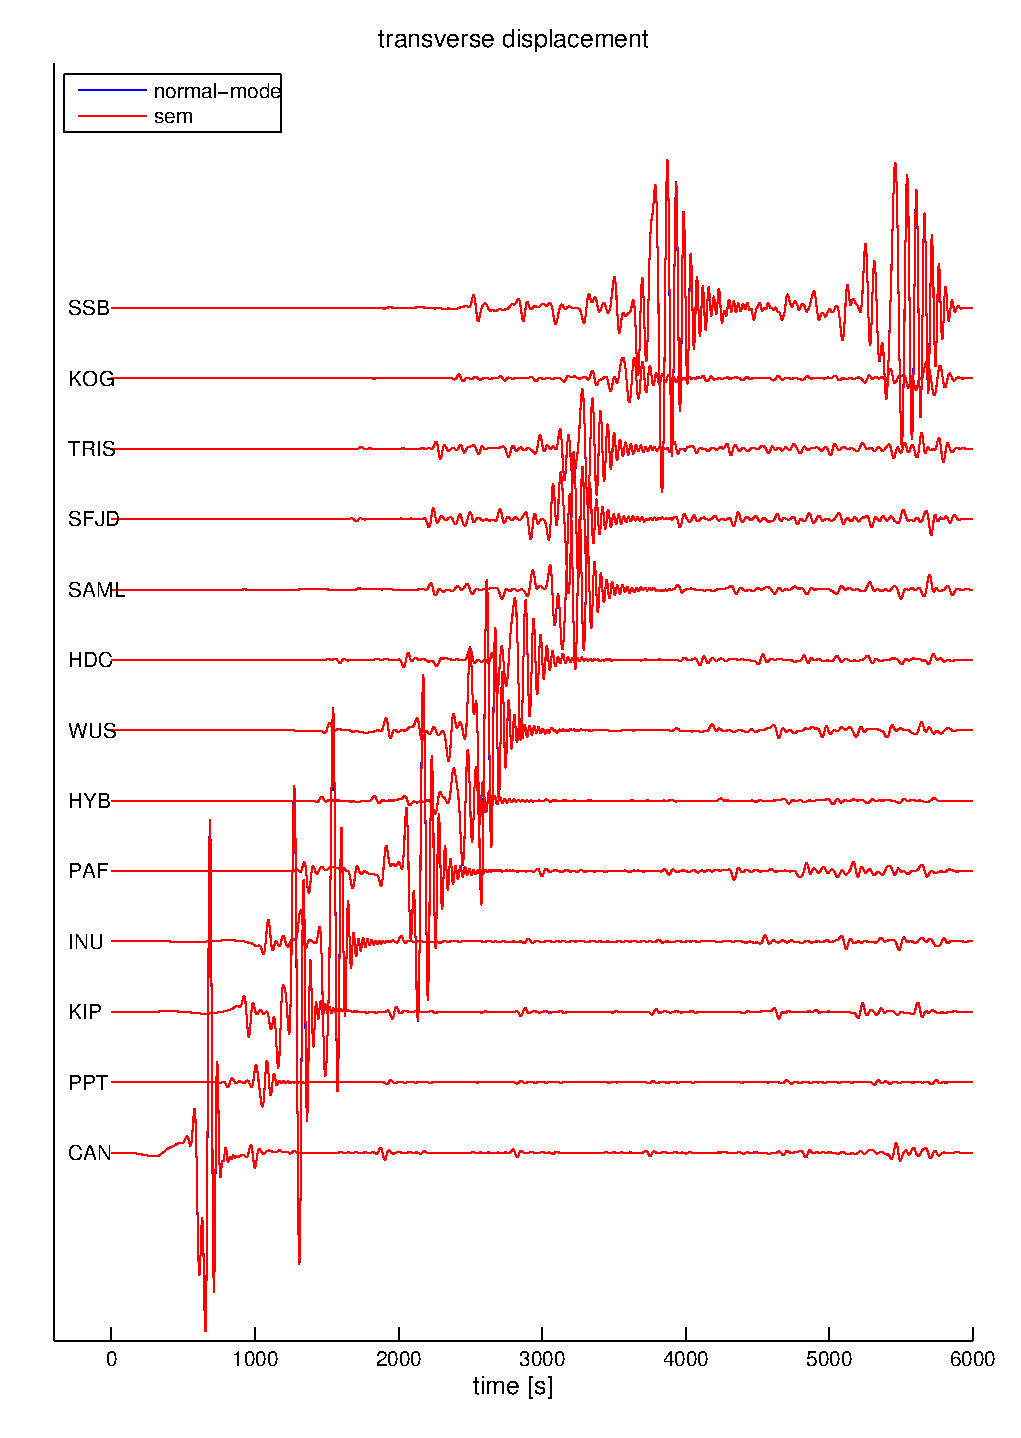
\includegraphics[scale=0.75]{figures/vanuatu_trans.pdf}
\caption{Same as in Figure \ref{fig:Vanuatu-with-Vertical}
for the transverse displacements.}
\label{fig:Vanuatu-with-Transverse}

\par\end{centering}
\end{figure}
%
\begin{figure}[ht]
\noindent \begin{centering}
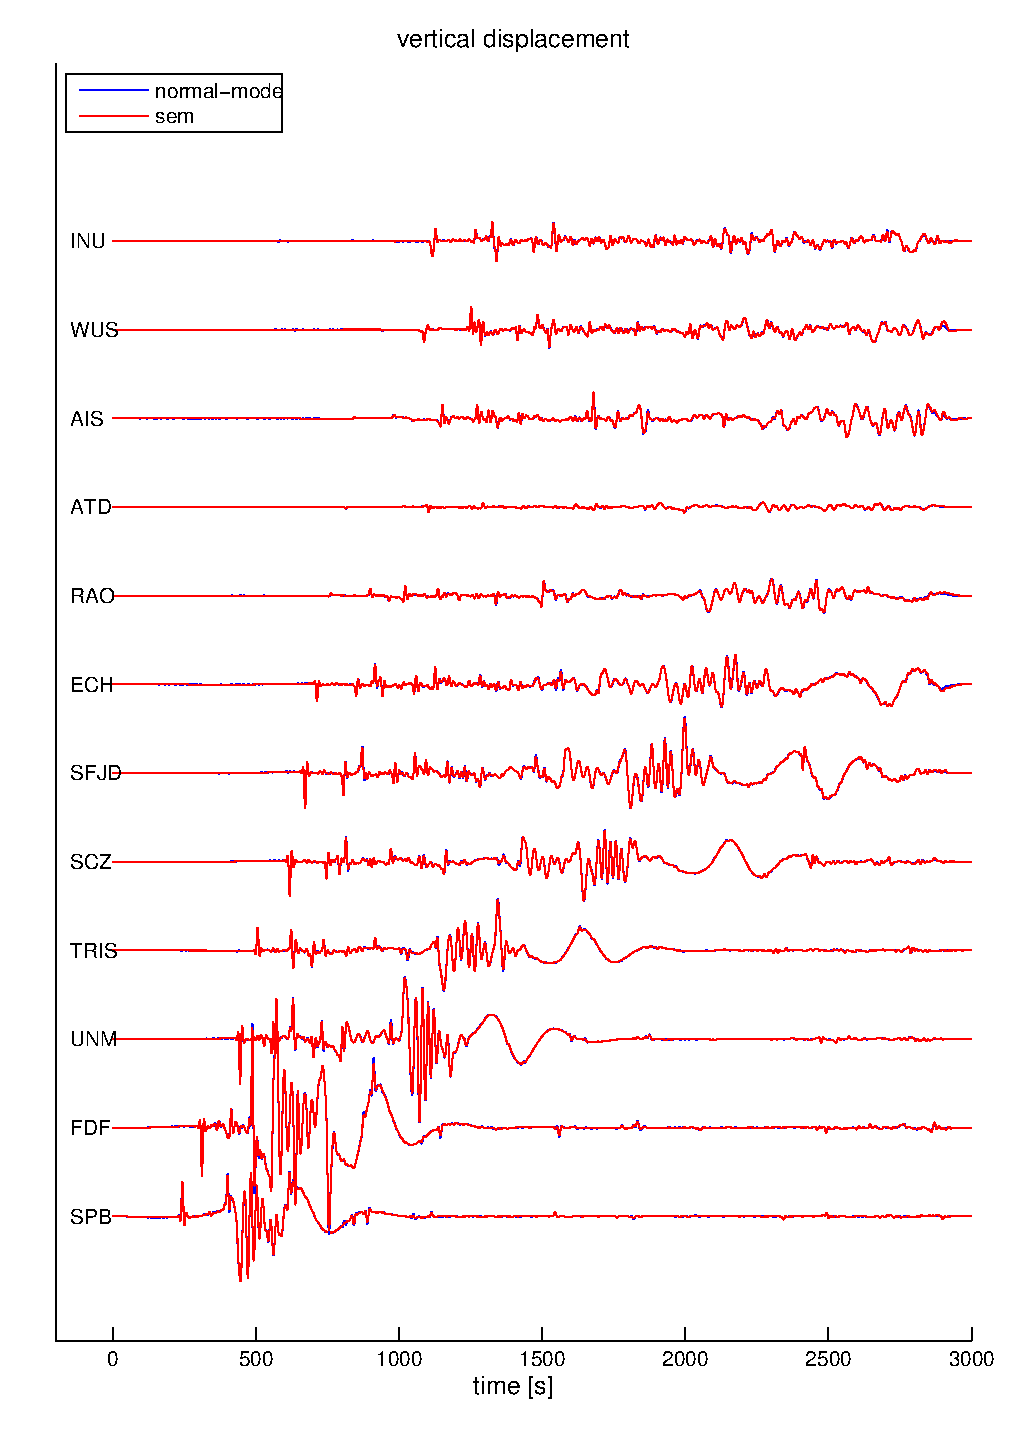
\includegraphics[scale=0.75]{figures/bolivia_vertical.pdf}
\caption{Normal-mode (blue) and SEM (red)
vertical displacements in transversely isotropic PREM considering
the effects of self-gravitation and attenuation for 12 stations at
increasing distance from the 1994 June 9th Bolivia event located at
647~km depth. The SEM computation is accurate for periods longer
than 9~s. The seismograms have been filtered between 10~s and 500~s.
The station names are indicated on the left.}
\label{fig:Bolivia-with-Vertical}

\par\end{centering}
\end{figure}
%
\begin{figure}[ht]
\noindent \begin{centering}
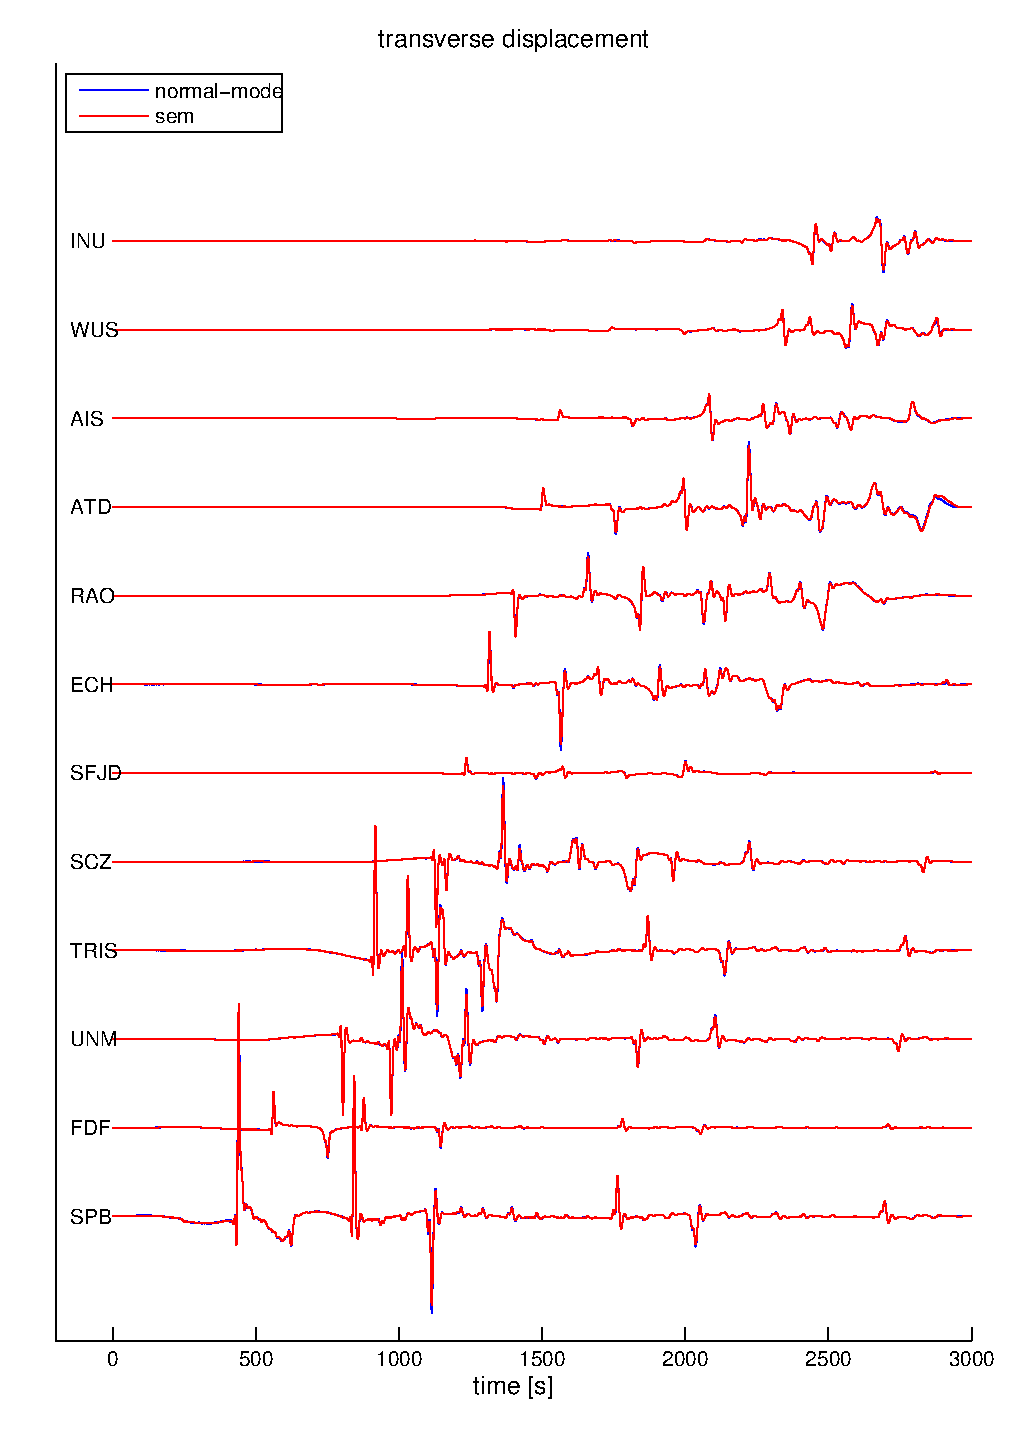
\includegraphics[scale=0.75]{figures/bolivia_trans.pdf}
\caption{Same as in Figure \ref{fig:Bolivia-with-Vertical}
for the transverse displacements.}
\label{fig:Bolivia-with-Transverse}

\par\end{centering}
\end{figure}


%
\begin{figure}[ht]
\noindent \begin{centering}
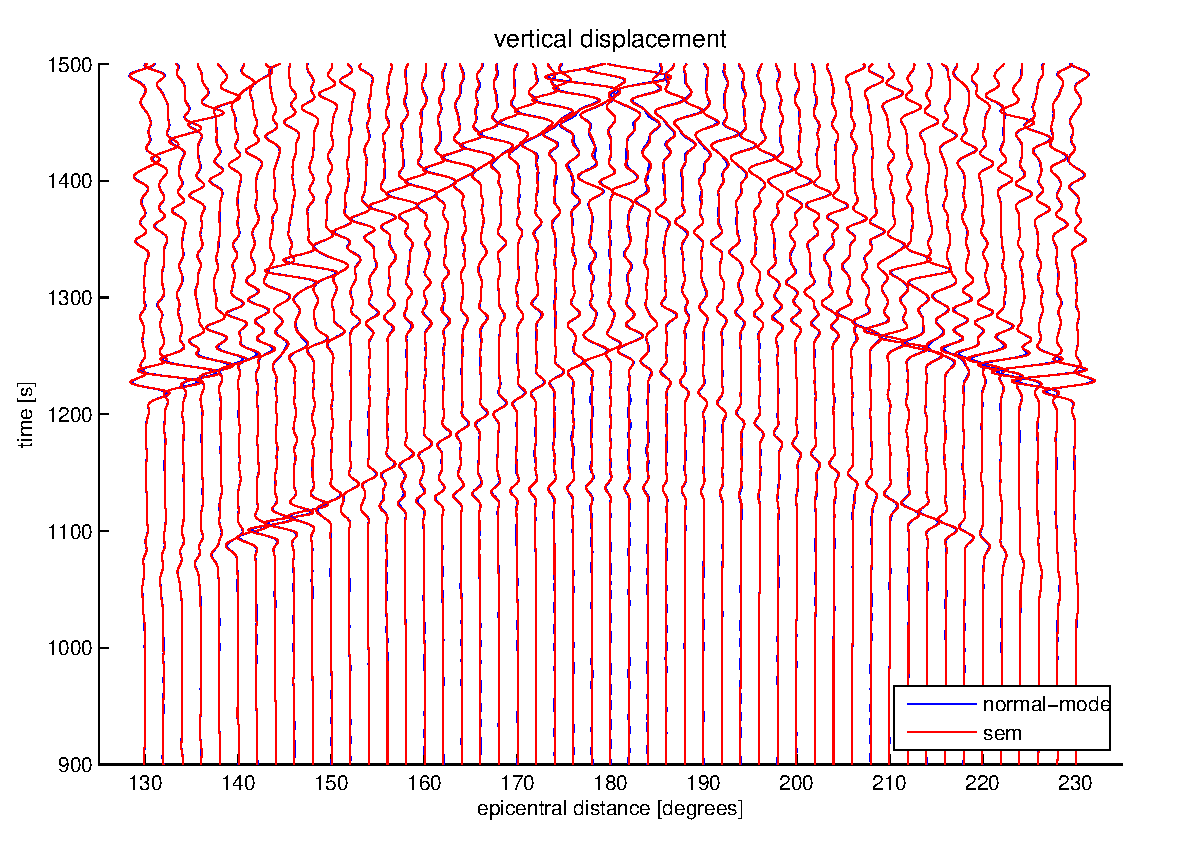
\includegraphics[scale=0.75]{figures/PKPdf_all_15s500s.pdf}
\caption{Seismograms recorded between 130 degrees and
230 degrees, showing in particular the good agreement for core phases
such as PKP. This figure is similar to Figure 24 of \citet{KoTr02a}.
The results have been filtered between 15~s and 500~s.}
\label{fig:Bolivia-PKP}

\par\end{centering}
\end{figure}


The normal-mode synthetics are calculated with the code \texttt{QmXD}
using mode catalogs with a shortest period of 8~s generated by the
code \texttt{OBANI}. No free-air, tilt, or gravitational potential
corrections were applied \citep{DaTr98}. We also turned off the effect
of the oceans in \texttt{QmXD}.\newline


The normal-mode and SEM displacement seismograms are first calculated
for a step source-time function, i.e., setting the parameter \texttt{half}
\texttt{duration} in the \texttt{CMTSOLUTION} file to zero for the
SEM simulations. Both sets of seismograms are subsequently convolved
with a triangular source-time function using the processing script \newline
\texttt{utils/seis\_process/process\_syn.pl}. They are also band-pass filtered
and the horizontal components are rotated to the radial and transverse
directions (with the script \texttt{utils/seis\_process/rotate.pl}).\newline


The match between the normal-mode and SEM seismograms is quite remarkable
for the experiment with attenuation, considering the very different
implementations of attenuation in the two computations (e.g., frequency
domain versus time domain, constant Q versus absorption bands).\newline


Further tests can be found in the \texttt{EXAMPLES} directory. It
contains the normal-mode and SEM seismograms, and the parameters (\texttt{STATIONS},
\texttt{CMTSOLUTION} and \texttt{Par\_file}) for the SEM simulations.\newline


Important remark: when comparing SEM results to normal mode results, one needs to
convert source and receiver coordinates from geographic to geocentric coordinates,
because on the equator the geographic and
geocentric latitude are identical but not elsewhere. Even for
spherically-symmetric simulations one must perform this conversion
because the source and receiver locations provided by www.globalCMT.org and
IRIS involve geographic coordinates.






\chapter{SAC Headers}\label{cha:SAC-headers}

Information about the simulation (i.e., event/station information, sampling rate, etc.)
is written in the header of the seismograms in SAC format.
The list of values and related explanation are given in Figure \ref{fig:SAC-headers}.
Please check the \href{http://www.iris.edu/software/sac/}{SAC webpages} for further information.
Please note that the reference time KZTIME is the centroid time ($t_\text{CMT}=t_\text{PDE}+\texttt{time shift}$)
which corresponds to zero time in the synthetics.
For kinematic rupture simulations, KZTIME is equal to the CMT time of the source having the minimum time-shift
in the \texttt{CMTSOLUTION} file, and coordinates, depth and half-duration of the event are not provided in the headers.
%
\begin{figure}[htp]
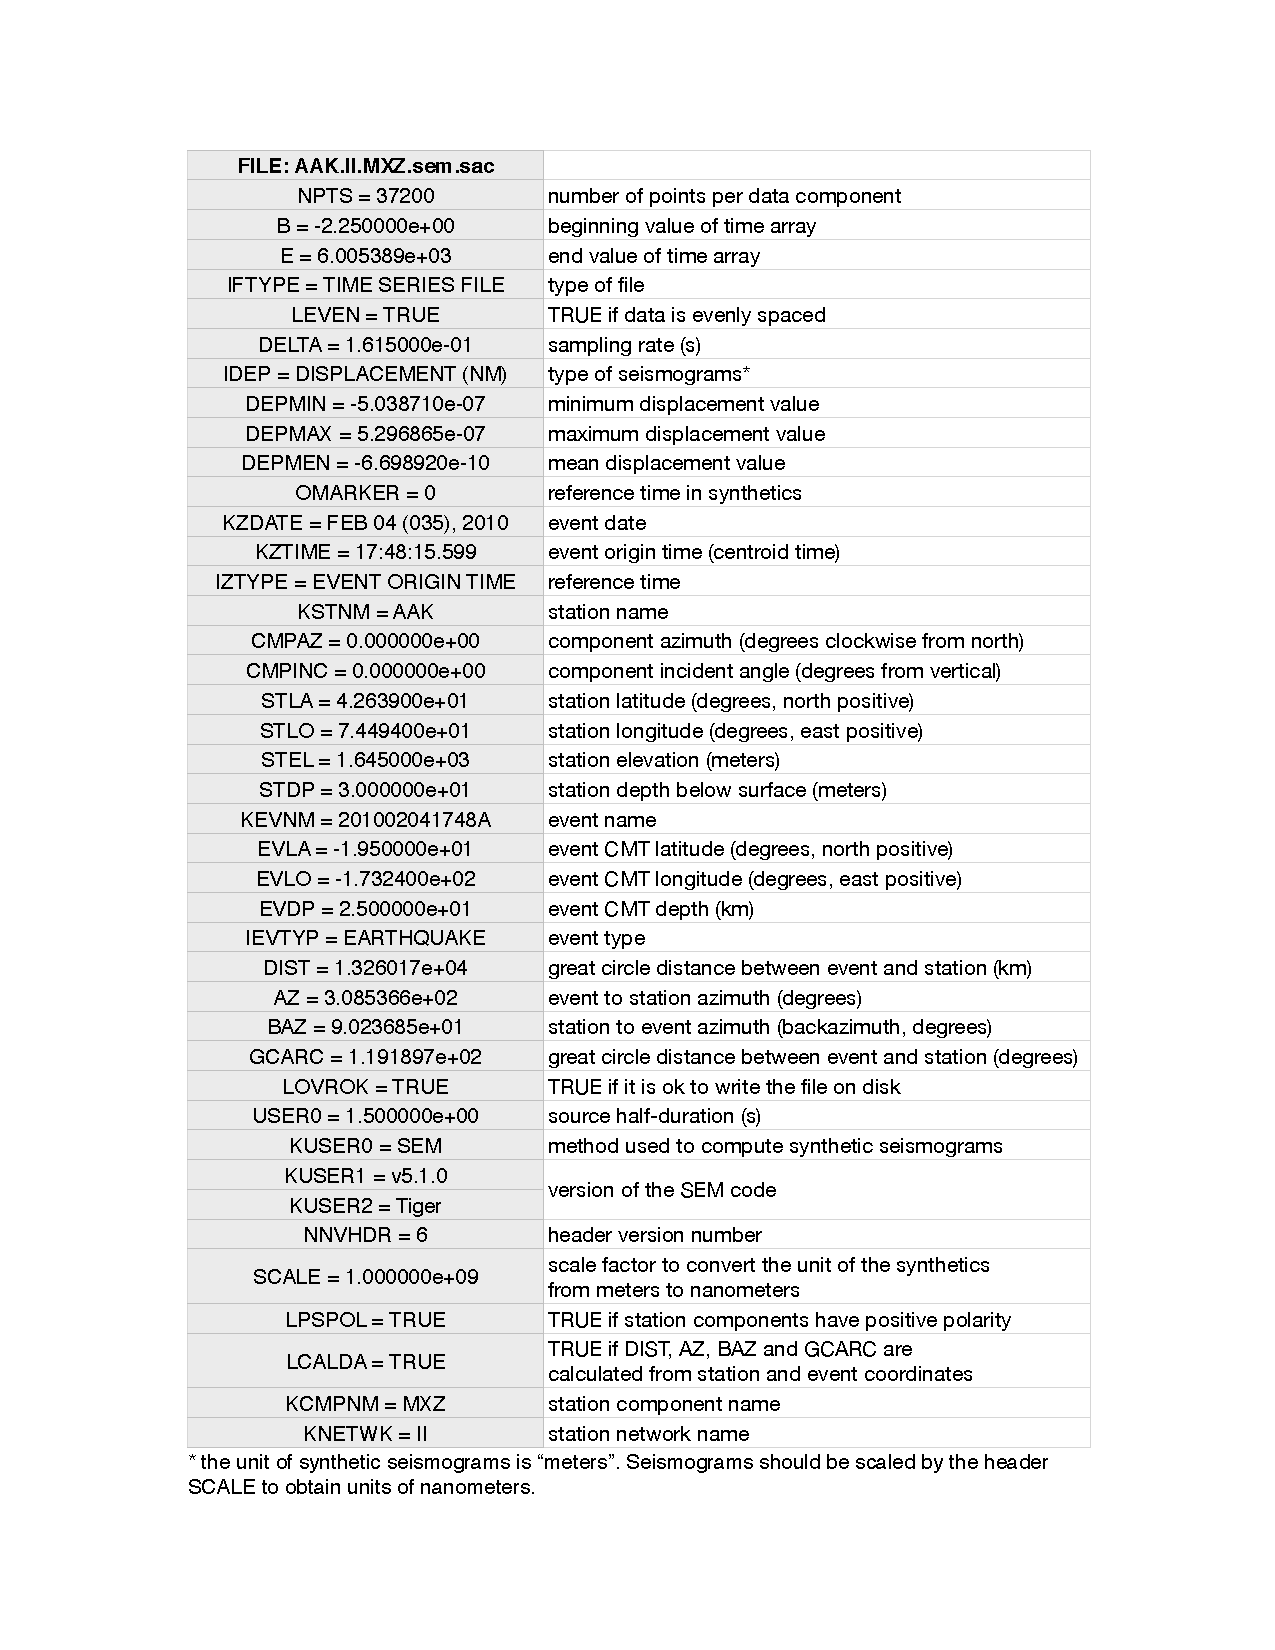
\includegraphics[scale=0.85]{figures/headers_sem_explained.pdf}
\caption{List of SAC headers and their explanations for a sample seismogram.}
\label{fig:SAC-headers}
\end{figure}






\chapter{Channel Codes of Seismograms}\label{cha:channel-codes}

Seismic networks, such as the Global Seismographic Network (GSN), generally involve various types of instruments with different
bandwidths, sampling properties and component configurations.
There are standards to name channel codes depending on instrument properties. IRIS (\url{http://www.iris.edu}) uses SEED/FDSN format
for channel codes, which are represented by three letters, such as \texttt{LHN}, \texttt{BHZ}, etc. In older versions of the
SPECFEM package, a common format was used for the channel codes of all seismograms, which was \texttt{LHE/LHN/LHZ}
for three components. To avoid confusion when comparisons are made to observed data, we are now using the FDSN convention
for SEM seismograms. In the following, we give a brief explanation of the FDSN convention and how it is adopted in SEM seismograms.
Please visit \url{http://www.iris.edu/manuals/SEED_appA.htm} for further information.\newline


\noindent
\textbf{\texttt{Band code:}} The first letter in the channel code denotes the band code of seismograms, which depends on the response band and the sampling rate of instruments. The list of band codes used by IRIS is shown in Figure \ref{fig:IRIS_band_codes}. The sampling rate of SEM synthetics is controlled by the resolution of simulations rather than instrument properties. However, for consistency, we follow the FDSN convention for SEM seismograms governed by their sampling rate. For SEM synthetics, we consider band codes for which $dt \leq 1$ s. The FDSN convention also considers the response band of instruments. For instance, short-period and broad-band seismograms with the same sampling rate correspond to different band codes, such as S and B, respectively. In such cases, we consider SEM seismograms as broad band, ignoring the corner period ($\geq 10$ s) of the response band of instruments (note that at these resolutions, the minimum period in the SEM synthetics will be less than $10$ s).
Accordingly, when you run a simulation the band code will be chosen depending on the resolution of the synthetics, and channel codes of SEM seismograms will start with either \texttt{L}, \texttt{M}, \texttt{B}, \texttt{H}, \texttt{C} or \texttt{F}, shown by red color in the figure.\newline

\begin{figure}[ht]
\noindent \begin{centering}
\includegraphics[scale=0.6]{figures/IRIS_band_codes.pdf}
\caption{The FDSN band code convention is based on the sampling rate
and the response band of instruments.
Please visit \url{http://www.iris.edu/manuals/SEED_appA.htm}
for further information. Grey rows show the relative band-code range in SPECFEM,
and the band codes used to name SEM seismograms are denoted in red.}
\label{fig:IRIS_band_codes}
\par\end{centering}
\end{figure}

\noindent
\textbf{\texttt{Instrument code:}} The second letter in the channel code corresponds to instrument codes, which specify the family to which the sensor belongs. For instance, \texttt{H} and \texttt{L} are used for high-gain and low-gain seismometers, respectively. The instrument code of SEM seismograms will always be \texttt{X}, as assigned by FDSN for synthetic seismograms. \newline


\noindent
\textbf{\texttt{Orientation code:}} The third letter in channel codes is an orientation code, which generally describes the physical configuration of the components of instrument packages. SPECFEM uses the traditional orientation code  \texttt{E/N/Z} (East-West, North-South, Vertical) for three components. \newline


\noindent
\textbf{\texttt{EXAMPLE:}} Depending on the resolution of your simulations, if the sampling rate is greater than $0.1$ s and less than $1$ s, a seismogram recorded on the vertical component of station \texttt{AAK} will be named \texttt{IU.AAK.MXZ.sem.sac}, whereas it will be \texttt{IU.AAK.BXZ.sem.sac}, if the sampling rate is greater than 0.0125 and less equal to 0.1 s.





\chapter{Troubleshooting}\label{cha:Troubleshooting}

\section*{FAQ}

\begin{description}
\item [configuration fails:]
Examine the log file 'config.log'. It contains detailed informations.
In many cases, the path's to these specific compiler commands F90,
CC and MPIF90 won't be correct if `./configure` fails.\newline


Please make sure that you have a working installation of a Fortran compiler,
a C compiler and an MPI implementation. You should be able to compile this
little program code:\newline

{\footnotesize
\begin{verbatim}
  program main
  include 'mpif.h'
  integer, parameter :: CUSTOM_MPI_TYPE = MPI_REAL
  integer ier
  call MPI_INIT(ier)
  call MPI_BARRIER(MPI_COMM_WORLD,ier)
  call MPI_FINALIZE(ier)
  end
\end{verbatim}
}

\item [compilation fails:]
In case a compilation error like the following occurs, stating

{\footnotesize
\begin{verbatim}
  ...
  obj/meshfem3D.o: In function `MAIN__':
  meshfem3D.f90:(.text+0x14): undefined reference to `_gfortran_set_std'
  ...
\end{verbatim}
}
\noindent
make sure you're pointing to the right 'mpif90' wrapper command.\newline


Normally, this message will appear when you are mixing two different Fortran
compilers. That is, using e.g. gfortran to compile non-MPI files
and mpif90, wrapper provided for e.g. ifort, to compile MPI-files.\newline


fix: e.g. specify
\begin{verbatim}
./configure FC=gfortran MPIF90=/usr/local/openmpi-gfortran/bin/mpif90
\end{verbatim}

\item [changing PPM model routines fails:]
In case you want to modify the PPM-routines in file \texttt{model\_ppm.f90}, please consider the following points:

\begin{enumerate}
\item Please check in file \texttt{get\_model\_parameter.f90} that the entry for PPM models looks like:

{\footnotesize
\begin{verbatim}
  ...
  else if(MODEL_ROOT == 'PPM') then
   ! overimposed based on isotropic-prem
   CASE_3D = .true.
   CRUSTAL = .true.
   MODEL_3D_MANTLE_PERTUBATIONS = .true.
   ONE_CRUST = .true.
   THREE_D_MODEL = THREE_D_MODEL_PPM
   TRANSVERSE_ISOTROPY = .true. ! to use transverse-isotropic prem
  ...
\end{verbatim}
}

\noindent
You can set \texttt{TRANSVERSE\_ISOTROPY} to \texttt{.false.} in case you want to use the isotropic PREM
as 1D background model.\newline

\item Transverse isotropy would mean different values for horizontal and vertically polarized wave speeds,
i.e. different for vph and   vpv, vsh and vsv, and it includes an additional parameter eta.
By default, we take these wave speeds from PREM and add your model perturbations to them.
For the moment, your model perturbations are added as isotropic perturbations, using the same dvp for vph and vpv,
and dvs for vsh   and vsv, see in \texttt{meshfem3D\_models.f90}:

{\footnotesize
\begin{verbatim}
  ...
   case(THREE_D_MODEL_PPM )
     ! point profile model
     call model_PPM(r_used,theta,phi,dvs,dvp,drho)
     vpv=vpv*(1.0d0+dvp)
     vph=vph*(1.0d0+dvp)
     vsv=vsv*(1.0d0+dvs)
     vsh=vsh*(1.0d0+dvs)
     rho=rho*(1.0d0+drho)
  ...
\end{verbatim}
}

\noindent
You could modify this to add different perturbations for vph and vpv, resp. vsh and vsv.
This would basically mean that you add transverse isotropic perturbations.
You can see how this is done with e.g. the model \texttt{s362ani},
following the flag \texttt{THREE\_D\_MODEL\_S362ANI} on how to modify accordingly the file \texttt{meshfem3D\_models.f90}.\newline


In case you want to add more specific model routines, follow the code sections starting with:

{\footnotesize
\begin{verbatim}
  !---
  !
  ! ADD YOUR MODEL HERE
  !
  !---
\end{verbatim}
}

\noindent
to see code sections sensitive to model updates.

  \end{enumerate}

\end{description}





\chapter{License}\label{cha:License}

\textbf{GNU GENERAL PUBLIC LICENSE Version 2, June 1991. Copyright
(C) 1989, 1991 Free Software Foundation, Inc. 59 Temple Place, Suite
330, Boston, MA 02111-1307 USA} \\
Everyone is permitted to copy and distribute verbatim copies of this
license document, but changing it is not allowed.


\section*{Preamble}

The licenses for most software are designed to take away your freedom
to share and change it. By contrast, the GNU General Public License
is intended to guarantee your freedom to share and change free software
-- to make sure the software is free for all its users. This General
Public License applies to most of the Free Software Foundation's software
and to any other program whose authors commit to using it. (Some other
Free Software Foundation software is covered by the GNU Library General
Public License instead.) You can apply it to your programs, too.

When we speak of free software, we are referring to freedom, not price.
Our General Public Licenses are designed to make sure that you have
the freedom to distribute copies of free software (and charge for
this service if you wish), that you receive source code or can get
it if you want it, that you can change the software or use pieces
of it in new free programs; and that you know you can do these things.

To protect your rights, we need to make restrictions that forbid anyone
to deny you these rights or to ask you to surrender the rights. These
restrictions translate to certain responsibilities for you if you
distribute copies of the software, or if you modify it.

For example, if you distribute copies of such a program, whether gratis
or for a fee, you must give the recipients all the rights that you
have. You must make sure that they, too, receive or can get the source
code. And you must show them these terms so they know their rights.

We protect your rights with two steps:

\begin{enumerate}
\item Copyright the software, and
\item Offer you this license which gives you legal permission to copy, distribute
and/or modify the software.
\end{enumerate}
Also, for each author's protection and ours, we want to make certain
that everyone understands that there is no warranty for this free
software. If the software is modified by someone else and passed on,
we want its recipients to know that what they have is not the original,
so that any problems introduced by others will not reflect on the
original authors' reputations.

Finally, any free program is threatened constantly by software patents.
We wish to avoid the danger that redistributors of a free program
will individually obtain patent licenses, in effect making the program
proprietary. To prevent this, we have made it clear that any patent
must be licensed for everyone's free use or not licensed at all.

The precise terms and conditions for copying, distribution and modification
follow.


\section*{GNU GENERAL PUBLIC LICENSE TERMS AND CONDITIONS FOR COPYING, DISTRIBUTION
AND MODIFICATION }

\begin{itemize}

\item[0.]This License applies to any program or other work which
contains a notice placed by the copyright holder saying it may be
distributed under the terms of this General Public License. The ``Program''
below refers to any such program or work, and a ``work based on the
Program'' means either the Program or any derivative work under copyright
law: that is to say, a work containing the Program or a portion of
it, either verbatim or with modifications and/or translated into another
language. (Hereinafter, translation is included without limitation
in the term ``modification.'') Each licensee is addressed as ``you.''\\
\\
Activities other than copying, distribution and modification are not
covered by this License; they are outside its scope. The act of running
the Program is not restricted, and the output from the Program is
covered only if its contents constitute a work based on the Program
(independent of having been made by running the Program). Whether
that is true depends on what the Program does.

\end{itemize}

\begin{enumerate}
\item You may copy and distribute verbatim copies of the Program's source
code as you receive it, in any medium, provided that you conspicuously
and appropriately publish on each copy an appropriate copyright notice
and disclaimer of warranty; keep intact all the notices that refer
to this License and to the absence of any warranty; and give any other
recipients of the Program a copy of this License along with the Program.


You may charge a fee for the physical act of transferring a copy,
and you may at your option offer warranty protection in exchange for
a fee.

\item You may modify your copy or copies of the Program or any portion of
it, thus forming a work based on the Program, and copy and distribute
such modifications or work under the terms of Section 1 above, provided
that you also meet all of these conditions:

\begin{enumerate}
\item You must cause the modified files to carry prominent notices stating
that you changed the files and the date of any change.
\item You must cause any work that you distribute or publish, that in whole
or in part contains or is derived from the Program or any part thereof,
to be licensed as a whole at no charge to all third parties under
the terms of this License.
\item If the modified program normally reads commands interactively when
run, you must cause it, when started running for such interactive
use in the most ordinary way, to print or display an announcement
including an appropriate copyright notice and a notice that there
is no warranty (or else, saying that you provide a warranty) and that
users may redistribute the program under these conditions, and telling
the user how to view a copy of this License. (Exception: if the Program
itself is interactive but does not normally print such an announcement,
your work based on the Program is not required to print an announcement.)
\end{enumerate}
These requirements apply to the modified work as a whole. If identifiable
sections of that work are not derived from the Program, and can be
reasonably considered independent and separate works in themselves,
then this License, and its terms, do not apply to those sections when
you distribute them as separate works. But when you distribute the
same sections as part of a whole which is a work based on the Program,
the distribution of the whole must be on the terms of this License,
whose permissions for other licensees extend to the entire whole,
and thus to each and every part regardless of who wrote it.

Thus, it is not the intent of this section to claim rights or contest
your rights to work written entirely by you; rather, the intent is
to exercise the right to control the distribution of derivative or
collective works based on the Program.

In addition, mere aggregation of another work not based on the Program
with the Program (or with a work based on the Program) on a volume
of a storage or distribution medium does not bring the other work
under the scope of this License.

\item You may copy and distribute the Program (or a work based on it, under
Section 2) in object code or executable form under the terms of Sections
1 and 2 above provided that you also do one of the following:

\begin{enumerate}
\item Accompany it with the complete corresponding machine-readable source
code, which must be distributed under the terms of Sections 1 and
2 above on a medium customarily used for software interchange; or,
\item Accompany it with a written offer, valid for at least three years,
to give any third party, for a charge no more than your cost of physically
performing source distribution, a complete machine-readable copy of
the corresponding source code, to be distributed under the terms of
Sections 1 and 2 above on a medium customarily used for software interchange;
or,
\item Accompany it with the information you received as to the offer to
distribute corresponding source code. (This alternative is allowed
only for noncommercial distribution and only if you received the program
in object code or executable form with such an offer, in accord with
Subsection b above.)
\end{enumerate}
The source code for a work means the preferred form of the work for
making modifications to it. For an executable work, complete source
code means all the source code for all modules it contains, plus any
associated interface definition files, plus the scripts used to control
compilation and installation of the executable. However, as a special
exception, the source code distributed need not include anything that
is normally distributed (in either source or binary form) with the
major components (compiler, kernel, and so on) of the operating system
on which the executable runs, unless that component itself accompanies
the executable.

If distribution of executable or object code is made by offering access
to copy from a designated place, then offering equivalent access to
copy the source code from the same place counts as distribution of
the source code, even though third parties are not compelled to copy
the source along with the object code.

\item You may not copy, modify, sublicense, or distribute the Program except
as expressly provided under this License. Any attempt otherwise to
copy, modify, sublicense or distribute the Program is void, and will
automatically terminate your rights under this License. However, parties
who have received copies, or rights, from you under this License will
not have their licenses terminated so long as such parties remain
in full compliance.
\item You are not required to accept this License, since you have not signed
it. However, nothing else grants you permission to modify or distribute
the Program or its derivative works. These actions are prohibited
by law if you do not accept this License. Therefore, by modifying
or distributing the Program (or any work based on the Program), you
indicate your acceptance of this License to do so, and all its terms
and conditions for copying, distributing or modifying the Program
or works based on it.
\item Each time you redistribute the Program (or any work based on the Program),
the recipient automatically receives a license from the original licensor
to copy, distribute or modify the Program subject to these terms and
conditions. You may not impose any further restrictions on the recipients'
exercise of the rights granted herein. You are not responsible for
enforcing compliance by third parties to this License.
\item If, as a consequence of a court judgment or allegation of patent infringement
or for any other reason (not limited to patent issues), conditions
are imposed on you (whether by court order, agreement or otherwise)
that contradict the conditions of this License, they do not excuse
you from the conditions of this License. If you cannot distribute
so as to satisfy simultaneously your obligations under this License
and any other pertinent obligations, then as a consequence you may
not distribute the Program at all. For example, if a patent license
would not permit royalty-free redistribution of the Program by all
those who receive copies directly or indirectly through you, then
the only way you could satisfy both it and this License would be to
refrain entirely from distribution of the Program.


If any portion of this section is held invalid or unenforceable under
any particular circumstance, the balance of the section is intended
to apply and the section as a whole is intended to apply in other
circumstances.

It is not the purpose of this section to induce you to infringe any
patents or other property right claims or to contest validity of any
such claims; this section has the sole purpose of protecting the integrity
of the free software distribution system, which is implemented by
public license practices. Many people have made generous contributions
to the wide range of software distributed through that system in reliance
on consistent application of that system; it is up to the author/donor
to decide if he or she is willing to distribute software through any
other system and a licensee cannot impose that choice.

This section is intended to make thoroughly clear what is believed
to be a consequence of the rest of this License.

\item If the distribution and/or use of the Program is restricted in certain
countries either by patents or by copyrighted interfaces, the original
copyright holder who places the Program under this License may add
an explicit geographical distribution limitation excluding those countries,
so that distribution is permitted only in or among countries not thus
excluded. In such case, this License incorporates the limitation as
if written in the body of this License.
\item The Free Software Foundation may publish revised and/or new versions
of the General Public License from time to time. Such new versions
will be similar in spirit to the present version, but may differ in
detail to address new problems or concerns.


Each version is given a distinguishing version number. If the Program
specifies a version number of this License which applies to it and
``any later version,'' you have the option of following the terms
and conditions either of that version or of any later version published
by the Free Software Foundation. If the Program does not specify a
version number of this License, you may choose any version ever published
by the Free Software Foundation.

\item If you wish to incorporate parts of the Program into other free programs
whose distribution conditions are different, write to the author to
ask for permission. For software which is copyrighted by the Free
Software Foundation, write to the Free Software Foundation; we sometimes
make exceptions for this. Our decision will be guided by the two goals
of preserving the free status of all derivatives of our free software
and of promoting the sharing and reuse of software generally.
\end{enumerate}

\subsection*{NO WARRANTY }

\begin{itemize}

\item[11.]BECAUSE THE PROGRAM IS LICENSED FREE OF CHARGE, THERE IS
NO WARRANTY FOR THE PROGRAM, TO THE EXTENT PERMITTED BY APPLICABLE
LAW. EXCEPT WHEN OTHERWISE STATED IN WRITING THE COPYRIGHT HOLDERS
AND/OR OTHER PARTIES PROVIDE THE PROGRAM ``AS IS'' WITHOUT WARRANTY
OF ANY KIND, EITHER EXPRESSED OR IMPLIED, INCLUDING, BUT NOT LIMITED
TO, THE IMPLIED WARRANTIES OF MERCHANTABILITY AND FITNESS FOR A PARTICULAR
PURPOSE. THE ENTIRE RISK AS TO THE QUALITY AND PERFORMANCE OF THE
PROGRAM IS WITH YOU. SHOULD THE PROGRAM PROVE DEFECTIVE, YOU ASSUME
THE COST OF ALL NECESSARY SERVICING, REPAIR OR CORRECTION.

\item[12.]IN NO EVENT UNLESS REQUIRED BY APPLICABLE LAW OR AGREED
TO IN WRITING WILL ANY COPYRIGHT HOLDER, OR ANY OTHER PARTY WHO MAY
MODIFY AND/OR REDISTRIBUTE THE PROGRAM AS PERMITTED ABOVE, BE LIABLE
TO YOU FOR DAMAGES, INCLUDING ANY GENERAL, SPECIAL, INCIDENTAL OR
CONSEQUENTIAL DAMAGES ARISING OUT OF THE USE OR INABILITY TO USE THE
PROGRAM (INCLUDING BUT NOT LIMITED TO LOSS OF DATA OR DATA BEING RENDERED
INACCURATE OR LOSSES SUSTAINED BY YOU OR THIRD PARTIES OR A FAILURE
OF THE PROGRAM TO OPERATE WITH ANY OTHER PROGRAMS), EVEN IF SUCH HOLDER
OR OTHER PARTY HAS BEEN ADVISED OF THE POSSIBILITY OF SUCH DAMAGES.

\end{itemize}


\section*{END OF TERMS AND CONDITIONS }


\subsection*{How to Apply These Terms to Your New Programs}

If you develop a new program, and you want it to be of the greatest
possible use to the public, the best way to achieve this is to make
it free software which everyone can redistribute and change under
these terms.

To do so, attach the following notices to the program. It is safest
to attach them to the start of each source file to most effectively
convey the exclusion of warranty; and each file should have at least
the ``copyright'' line and a pointer to where the full notice is found.
For example:

\begin{quote}
One line to give the program's name and a brief idea of what it does.
Copyright {\footnotesize $\copyright$ (}year) (name of author)

This program is free software; you can redistribute it and/or modify
it under the terms of the GNU General Public License as published
by the Free Software Foundation; either version 2 of the License,
or (at your option) any later version.

This program is distributed in the hope that it will be useful, but
WITHOUT ANY WARRANTY; without even the implied warranty of MERCHANTABILITY
or FITNESS FOR A PARTICULAR PURPOSE. See the GNU General Public License
for more details.

You should have received a copy of the GNU General Public License
along with this program; if not, write to the Free Software Foundation,
Inc., 59 Temple Place, Suite 330, Boston, MA 02111-1307 USA
\end{quote}
Also add information on how to contact you by electronic and paper
mail.

If the program is interactive, make it output a short notice like
this when it starts in an interactive mode:

\begin{quote}
Gnomovision version 69, Copyright $\copyright$ year name of author Gnomovision
comes with ABSOLUTELY NO WARRANTY; for details type `show w'. This
is free software, and you are welcome to redistribute it under certain
conditions; type `show c' for details.
\end{quote}
The hypothetical commands `show w' and `show c' should show the appropriate
parts of the General Public License. Of course, the commands you use
may be called something other than `show w' and `show c'; they could
even be mouse-clicks or menu items -- whatever suits your program.

You should also get your employer (if you work as a programmer) or
your school, if any, to sign a ``copyright disclaimer'' for the program,
if necessary. Here is a sample; alter the names:

\begin{quote}
Yoyodyne, Inc., hereby disclaims all copyright interest in the program
`Gnomovision' (which makes passes at compilers) written by James Hacker.

(signature of Ty Coon)\\
1 April 1989 \\
Ty Coon, President of Vice
\end{quote}
This General Public License does not permit incorporating your program
into proprietary programs. If your program is a subroutine library,
you may consider it more useful to permit linking proprietary applications
with the library. If this is what you want to do, use the GNU Library
General Public License instead of this License.




%%%%%%%%%%%%%%%%%%%%%%%%%%%%%%%%%%%%%%%%%%%

\end{document}
